\documentclass{article}
\usepackage[utf8]{inputenc}
\usepackage[T5]{fontenc}
\usepackage[vietnamese]{babel}
\usepackage[fontsize=13pt]{scrextend}
\usepackage{hyperref}
\usepackage[paperheight=29.7cm, paperwidth=21cm, right=2cm, left=3cm, top=2cm, bottom=2.5cm]{geometry}
\usepackage{mathptmx}
\usepackage{graphicx}
\usepackage{float}
\usepackage{tikz}
\usepackage{adjustbox}
\usetikzlibrary{calc}
\usepackage{indentfirst} % Thư viện thụt đầu dòng
\usepackage{setspace}
\renewcommand{\baselinestretch}{1.2} % Dãn dòng
\setlength{\parskip}{6pt}
% \setlength{\parindent}{1cm}
\usepackage{titlesec} % Thư viện set up các kiểu chữ
\usepackage{tcolorbox}
\usepackage{tocloft} % Gói để tuỳ chỉnh mục lục
\usepackage{changepage} % Gói adjustwidth
\usepackage{makecell}
\usepackage{xcolor}
\usepackage[table]{xcolor}

\usepackage{fancyhdr} % Import gói fancyhdr
\setcounter{secnumdepth}{4}
\usepackage{enumitem}

\renewcommand{\headrulewidth}{0.4pt}       % Đường kẻ header
\renewcommand{\footrulewidth}{0.4pt}       % Đường kẻ footer
\renewcommand{\cftsecleader}{\cftdotfill{\cftdotsep}} % Thêm dấu chấm trong mục lục

\pagestyle{fancy}
\fancyhf{} % Xóa header và footer mặc định
\fancyhead[L]{\textbf{IT3180 - Nhập môn công nghệ phần mềm}} % Header góc trái
\fancyfoot[L]{Nhóm 1} % Footer góc trái
\fancyfoot[R]{\thepage} % Footer góc phải

\titlespacing*{\section}{0pt}{0pt}{30pt} % Heading 1
\titleformat*{\section}{\fontsize{16pt}{0pt}\selectfont \bfseries \centering}

\titlespacing*{\subsection}{0pt}{10pt}{0pt} % Heading 2
\titleformat*{\subsection}{\fontsize{14pt}{0pt}\selectfont \bfseries}

\titlespacing*{\subsubsection}{0pt}{10pt}{0pt} % Heading 3
\titleformat*{\subsubsection}{\fontsize{13pt}{0pt}\selectfont \bfseries \itshape}

\titlespacing*{\paragraph}{0pt}{10pt}{0pt} % Heading 4
\titleformat*{\paragraph}{\fontsize{13pt}{0pt}\selectfont \itshape}

\newcommand{\Border}[0]
{
    \begin{tikzpicture}[overlay, remember picture]
    \draw[line width=3pt]
        ($ (current page.north west) + (3.0cm, -2.0cm) $)
        rectangle
        ($ (current page.south east) + (-2.0cm, 2.5cm) $);
    \draw[line width=0.5pt]
        ($ (current page.north west) + (3.1cm, -2.1cm) $)
        rectangle
        ($ (current page.south east) + (-2.1cm, 2.6cm) $);
    \end{tikzpicture}
}
\newcommand{\getpack}[3]
{
    \textit{#1}
    \begin{figure}[H]
        \centering
        \includegraphics[width=#2\linewidth]{#3}
    \end{figure}
}
\definecolor{lightblue}{HTML}{b3c5e6}
\definecolor{blueL}{HTML}{4371c3}
\newcommand{\setwhite}{\textcolor{white}}

\newcommand{\describetable}[2]
{
    \textit{#1}
    \begin{center}
        \begin{tabular}{|c|p{2.5cm}|p{2cm}|p{2cm}|p{2.5cm}|p{1.5cm}|}
            \hline
            \cellcolor{blueL}{\setwhite{Tên trường}} & 
            \cellcolor{blueL}{\setwhite{\makecell[c]{Kiểu dữ liệu}}} & \cellcolor{blueL}{\setwhite{Kích thước}} & 
            \cellcolor{blueL}{\setwhite{Ràng buộc}} \newline 
            \cellcolor{blueL}{\setwhite{toàn vẹn}} & 
            \cellcolor{blueL}{\setwhite{\makecell[c]{Khuôn dạng}}} & \cellcolor{blueL}{\setwhite{\makecell[c]{Ghi chú}}} \\
            \hline
            #2 
        \end{tabular}
    \end{center}
}
\newcommand{\getRowWithColor}[7]
{
    \cellcolor{#7}{#1} & 
    \cellcolor{#7}{#2} & 
    \cellcolor{#7}{#3} & 
    \cellcolor{#7}{#4} & 
    \cellcolor{#7}{#5} & 
    \cellcolor{#7}{#6} \\
    \hline
}

\makeatletter
\let\ps@plain\ps@fancy
\makeatother

\begin{document}
% % Bìa ---------------------------------------------------------------------------
% \begin{titlepage}
% \begin{Border}
%     \begin{center}
%         \vspace{-12pt} TRƯỜNG ĐẠI HỌC BÁCH KHOA HÀ NỘI \\
%         \textbf{VIỆN CÔNG NGHỆ THÔNG TIN VÀ TRUYỀN THÔNG} \\
%         \rule{0.8\textwidth}{0.5pt} \\[1cm]

%         \begin{figure}[H]
%             \centering
%             \includegraphics[width=1.53cm, height = 2.26cm]{image/Logo_Bách_Khoa.png}
%         \end{figure}
        
%         \textbf{\fontsize{24pt}{0pt}\selectfont BÀI TẬP LỚN} \\[0.5cm]
%         \textbf{\fontsize{14pt}{0pt}\selectfont MÔN: NHẬP MÔN CÔNG NGHỆ PHẦN MỀM} \\[1cm]
        
%         {\fontsize{20pt}{0pt} \selectfont \textbf{Quản lý thu phí, đóng góp}} \\[1cm]
        
%         \begin{tabular}{ll}
%         \textbf{\fontsize{14pt}{0pt}\selectfont Nhóm} & \fontsize{14pt}{0pt}\selectfont : 1 \\
%         \textbf{\fontsize{14pt}{0pt}\selectfont Mã lớp học} & \fontsize{14pt}{0pt}\selectfont : 154019 \\
%         \textbf{\fontsize{14pt}{0pt}\selectfont Giáo viên hướng dẫn} & \fontsize{14pt}{0pt}\selectfont : ThS. Nguyễn Mạnh Tuấn \\
%         \end{tabular} \\[1.5cm]
        
%         \textbf{\fontsize{14pt}{0pt}\selectfont Danh sách sinh viên thực hiện:} \\[1cm]
        
%         \begin{tabular}{|c|c|c|c|c|}
%             \hline
%             \textbf{STT} & \textbf{Họ tên} & \textbf{Mã sinh viên} & \textbf{Email} & \textbf{Lớp} \\ 
%             \hline
%             1 & Trương Minh Ngọc & 20220038 & ngoc.tm220038 & KTMT-01 \\ 
%             \hline
%             2 & Nguyễn Tùng Dương & 20224968 & duong.nt224968 & KTMT-01 \\ 
%             \hline
%             3 & Lê Huy Dũng & 20224960 & dung.lh224960 & KTMT-01 \\
%             \hline
%             4 & Nguyễn Khánh Huyền & 20225016 & huyen.nk225016 & KTMT-06 \\ 
%             \hline
%             5 & Đỗ Minh Phúc & 20225064 & phuc.dm225064 & KTMT-06 \\
%             \hline
%         \end{tabular}  

%         \vspace{1.5cm}
%         \fontsize{14pt}{0pt}\selectfont \textbf{Hà Nội, tháng 12 năm 2024}
%     \end{center}
% \end{Border}
% \end{titlepage}
% \newpage

% % Trang mục lục ---------------------------------------------------------------------------
% \renewcommand{\contentsname}{\textbf{MỤC LỤC}} % Đặt tên mục lục
% \renewcommand{\cfttoctitlefont}{\hfill\fontsize{16pt}{0pt}\selectfont\bfseries} % Căn giữa và đổi font chữ
% \renewcommand{\cftaftertoctitle}{\hfill} % Giữ căn giữa sau tiêu đề
% \addcontentsline{toc}{section}{MỤC LỤC} % Thêm mục lục vào bảng mục lục
% \tableofcontents % tạo mục lục tự động
% \cleardoublepage

% % Lời nói đầu ---------------------------------------------------------------------------
% \section*{LỜI NÓI ĐẦU}
% \addcontentsline{toc}{section}{LỜI NÓI ĐẦU}
% Quản lý thu chi là việc mà bất cứ khu phố, tổ dân phố,… đều phải giải quyết để
% giúp minh bạch thông tin, công khai các khoản thu, ghi chép và lưu trữ lại những
% thông tin nộp phí. Để giải quyết vấn đề này cần một phần mềm có thể thay thế hoàn
% toàn những cuốn sổ ghi tay để giúp ghi lại thông tin nộp phí từ người dân, tính toán
% khoản thu. Đề tài sẽ mô tả chi tiết về những bước xây dựng lên 1 phần mềm hỗ trợ
% quản lý thu phí 

% Để tiếp cận và hoàn thiện đề tài, nhóm em sử dụng HTML và CSS, Java Spring 
% Boot để xây dựng phần mềm UI trên Desktop hỗ trợ việc quản lý thu phí. Để quản lý thu phí được hiệu quả phần mềm cần hỗ trợ việc quản lý nhân khẩu, hộ khẩu và các khoản thu. Phần
% mềm xây dựng giúp thống kê các khoản nộp tiền, quản lý thông tin nhân khẩu, hộ khẩu, khoản thu và các khoản nộp.
% \newpage

% % Trang 2-----------------------------------------------------------

% \section*{PHÂN CÔNG THÀNH VIÊN TRONG NHÓM}
% \addcontentsline{toc}{section}{PHÂN CÔNG THÀNH VIÊN TRONG NHÓM}
% \begin{adjustwidth}{0cm}{1cm} % Lùi vào trái và phải 1cm
% \resizebox{\textwidth}{!}
% { % Đặt bảng vừa chiều rộng văn bản
% \begin{tabular}{|p{2.5cm}|p{3.5cm}|p{3cm}|p{4.5cm}|p{2.5cm}|}
% \hline
% \textbf{Họ và tên} & \textbf{Email} & \textbf{Điện thoại} & \textbf{Công việc thực hiện} & \textbf{Đánh giá} \\ 
% \hline
% Trương Minh Ngọc & ngoc.tm220038 & \textbf{0866137678} & Thiết kế cơ sở dữ liệu, Hỗ trợ, đóng góp xây dựng ý tưởng và tham gia làm báo cáo & Hoàn thành \\ 
% \hline
% Nguyễn Tùng Dương & duong.nt224968 & \textbf{0357981704} & Làm backend, tham gia làm báo cáo & Hoàn thành \\ 
% \hline
% Nguyễn Khánh Huyền & huyen.nk225016 & \textbf{0972950285} & Tham gia làm báo cáo & Hoàn thành \\ 
% \hline
% Lê Huy Dũng & dung.lh224960 & \textbf{0974187142} & Làm frontend, tham gia làm báo cáo & Hoàn thành \\ 
% \hline
% Đỗ Minh Phúc & phuc.dm225064 & \textbf{0963908468} & Làm frontend, tham gia làm báo cáo & Hoàn thành \\ 
% \hline
% \end{tabular}
% }
% \end{adjustwidth}
% \newpage

% % Trang 3 --------------------------------------------------------------------------
% \section*{CHƯƠNG 1. KHẢO SÁT BÀI TOÁN}
% \addcontentsline{toc}{section}{CHƯƠNG 1. KHẢO SÁT BÀI TOÁN}
% \setcounter{section}{1}
% \subsection{Mô tả yêu cầu bài toán}
% Bài toán quản lý thu phí, đóng góp (yêu cầu nghiệp vụ số 2)
% \begin{itemize}[leftmargin = 1.5cm]
%     \item Hàng năm tổ dân phố thực hiện thu một số khoản phí và đóng góp của các hộ gia đình, công việc này do cán bộ kế toán phụ trách. Khoản phí vệ sinh là bắt buộc với tất cả các hộ gia đình, mỗi năm thu 1 lần với định mức 6.000 VNĐ / 1 tháng / 1 nhân khẩu.
%     \item Cán bộ kế toán sẽ lập danh sách các hộ gia đình và số nhân khẩu tương ứng, sau đó đến từng nhà thu phí và ghi nhận số tiền nộp. Đối với các khoản đóng góp thì không quy định số tiền mà phụ thuộc vào từng hộ, các khoản đóng góp này được thu theo từng đợt của các cuộc vận động như: “Ủng hộ ngày thương binhliệt sỹ 27/07”, “Ủng hộ ngày tết thiếu nhi”, “Ủng hộ vì người nghèo”, Trợ giúp đồng bào bị ảnh hưởng bão lụt”,…
%     \item Cán bộ kế toán cũng cần thống kê tổng số tiền đã thu trong mỗi đợt, tổng số hộ đã nộp và có thể xem chi tiết mỗi hộ đã nộp những khoản tiền nào.
% \end{itemize}

% \subsection{Khảo sát bài toán}
% Một số mẫu quản lý thu phí có sẵn theo yêu cầu của bài toán được thu thập:

% \subsection{Xác định thông tin cơ bản cho nghiệp vụ của bài toán}
% Thông tin cơ bản cho nghiệp vụ bài toán:

% \subsection{Xây dựng biểu đồ mô tả nghiệp vụ và phân cấp chức năng}

% \subsection{Xây dựng kế hoạch dự án đơn giản}

% \newpage

% % Trang mới -----------------------------------------------------------------------
\section*{CHƯƠNG 2. ĐẶC TẢ YÊU CẦU BÀI TOÁN}
\addcontentsline{toc}{section}{CHƯƠNG 2. ĐẶC TẢ YÊU CẦU BÀI TOÁN}
\setcounter{section}{2}
\setcounter{subsection}{0}
\subsection{Giới thiệu chung}
Các tác nhân của hệ thống: 
\begin{itemize}
    \item[-] Người quản lý và cư dân là những người sử dụng hệ thống này, hệ thống được cung cấp thông tin từ nhân khẩu trong vùng quản lý
    \item[-] Người quản lý sẽ duy trì và quản trị hệ thống 
    \item[-] Cư dân sử dụng hệ thống để kiểm tra thông tin và nhận thông báo của chung cư
\end{itemize}

Bảng liệt kê các tác nhân và mô tả thông tin cho các tác nhân
\begin{figure}[H]
    \centering
    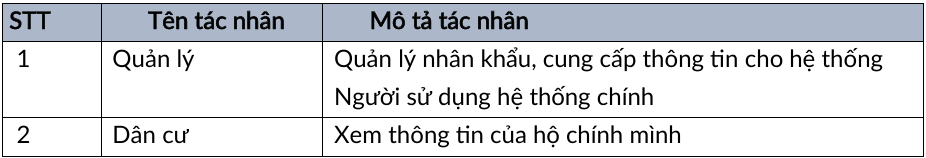
\includegraphics[width=15.53cm, height = 3cm]{Ảnh chương 2/Bảng tác nhân.png}
\end{figure}
Các Use Case cần thiết cho hệ thống và đặt mã cho các use-case
\begin{figure}[H]
    \centering
    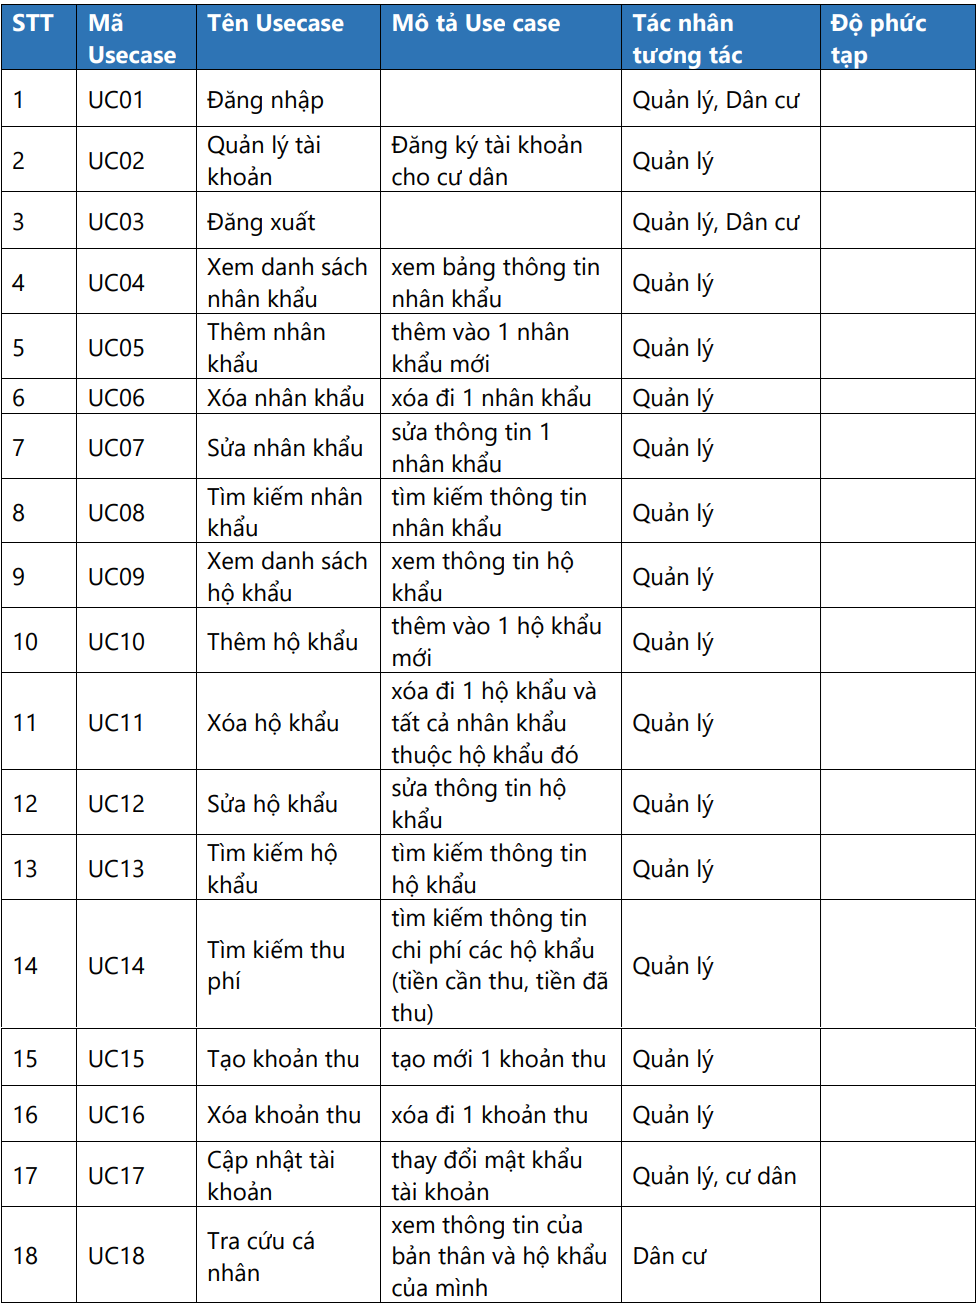
\includegraphics[width=0.9\textwidth]{Ảnh chương 2/Bảng usecase.png}
\end{figure}
\subsection{Biểu đồ use case} 
\subsubsection{Biểu đồ use case tổng quan}
Để truy cập vào ứng dụng, quản lý và cư dân sử dụng tài khoản và mật khẩu được cấp sẵn với vai trò khác nhau. \\
Quản lý được cấp quyền chỉnh sửa thông tin liên quan như hộ khẩu, nhân khẩu, khoản thu qua các tính năng của trang web.\\
Cư dân có thể dùng tài khoản được cấp để xem thông tin và nhận thông báo từ quản lý
\begin{figure}[H]
    \centering
    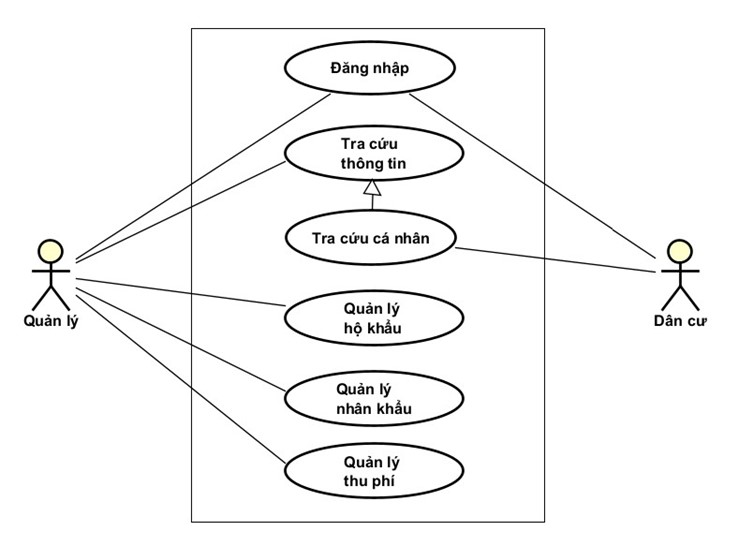
\includegraphics[width=12.53cm, height = 8cm]{Ảnh chương 2/Tổng quát.jpg}
\end{figure}
\subsubsection{Biểu đồ use case phân rã mức 2}
\begin{itemize}
    \item Phân rã Usecase "Đăng nhập"
    \begin{figure}[H]
        \centering
        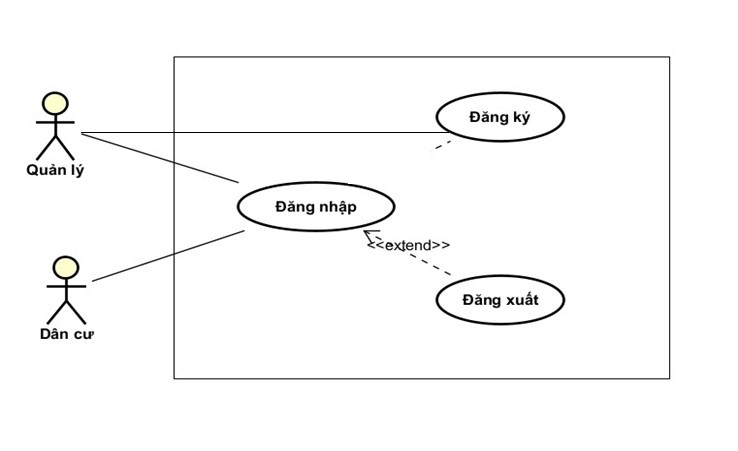
\includegraphics{Ảnh chương 2/Đăng nhập.jpg}
    \end{figure}
\vspace{5cm}
    \item Phân rã Usecase "Quản lý hộ khẩu"
    \begin{figure}[H]
        \centering
        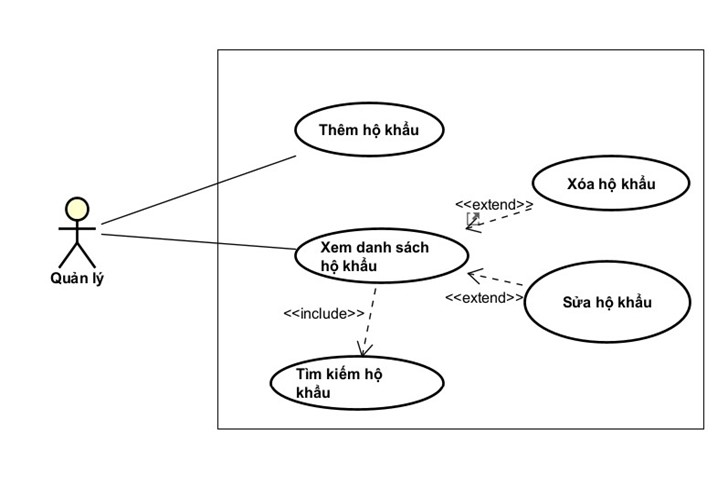
\includegraphics{Ảnh chương 2/Hộ khẩu.jpg}
    \end{figure}

    \item Phân rã Usecase "Quản lý nhân khẩu"
    \begin{figure}[H]
        \centering
        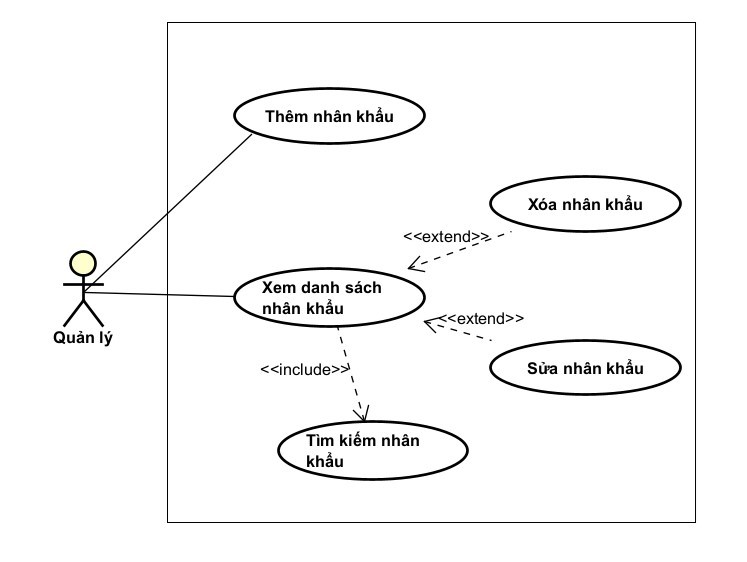
\includegraphics{Ảnh chương 2/Nhân khẩu.jpg}
    \end{figure}
    
    \vspace{1cm}
    \item Phân rã Usecase "Quản lý thu phí"
    \begin{figure}[H]
        \centering
        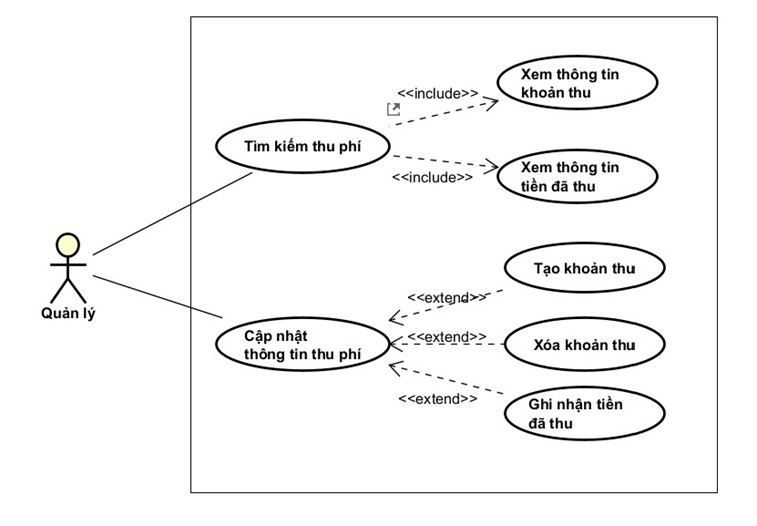
\includegraphics{Ảnh chương 2/Khoản thu.jpg}
    \end{figure}
\end{itemize}
\subsection{Đặc tả use case}
\begin{itemize}
    \item Đăng nhập và Đăng kí
    \begin{figure}[H]
        \centering
        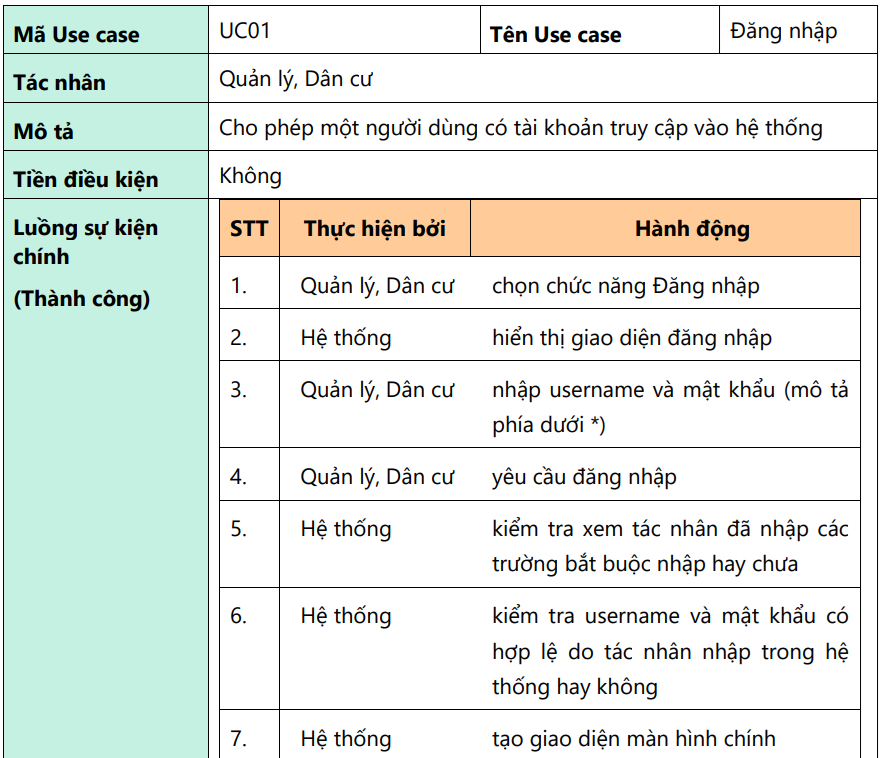
\includegraphics[width=0.8\textwidth]{Ảnh chương 2/UC01 1.png}
    \end{figure}
    \begin{figure}[H]
        \centering
        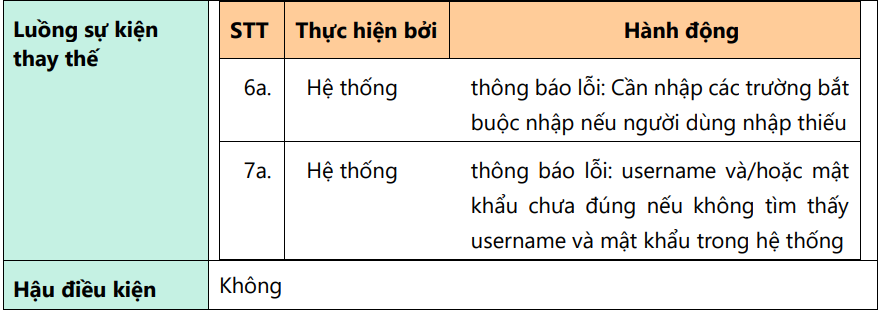
\includegraphics[width=0.8\textwidth]{Ảnh chương 2/UC01.png}
    \end{figure}
    \begin{figure}[H]
        \centering
        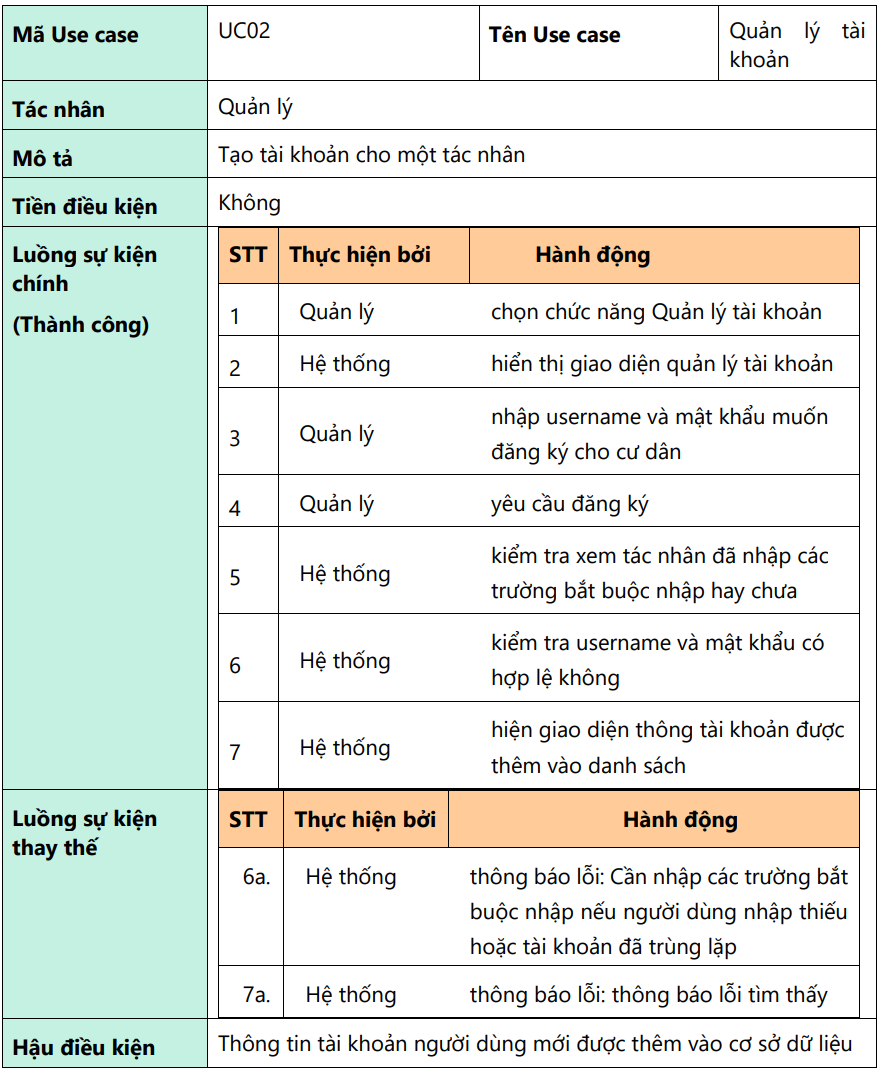
\includegraphics[width=0.8\textwidth]{Ảnh chương 2/UC02.png}
    \end{figure}
    \begin{figure}[H]
        \centering
        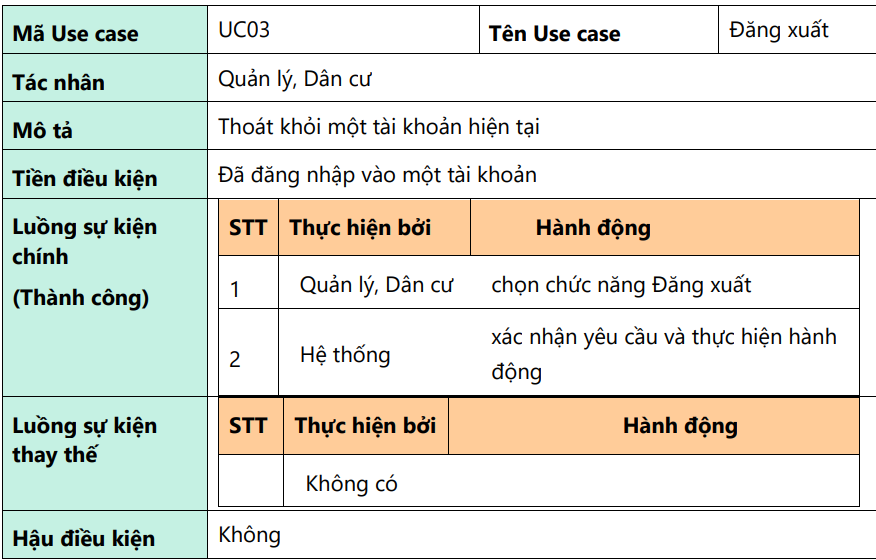
\includegraphics[width=0.8\textwidth]{Ảnh chương 2/UC03.png}
    \end{figure}
    \item Quản lý nhân khẩu
    \begin{figure}[H]
        \centering
        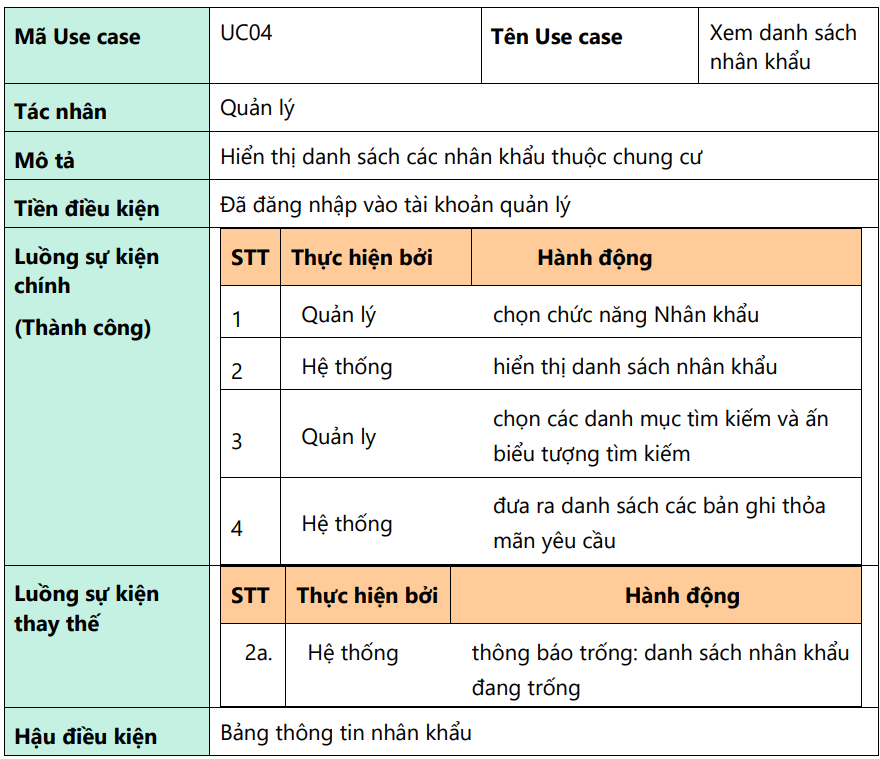
\includegraphics[width=0.8\textwidth]{Ảnh chương 2/UC04.png}
    \end{figure}
    \begin{figure}[H]
        \centering
        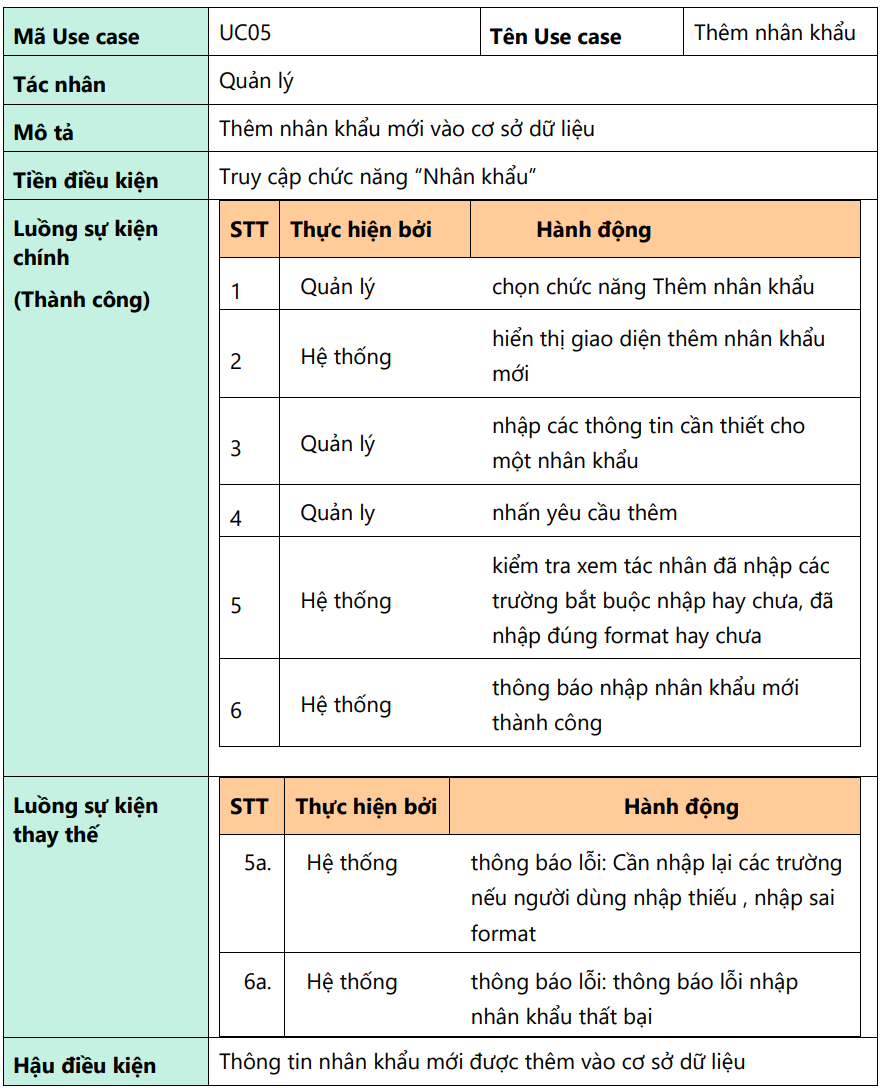
\includegraphics[width=0.8\textwidth]{Ảnh chương 2/UC05.png}
    \end{figure}
    \begin{figure}[H]
        \centering
        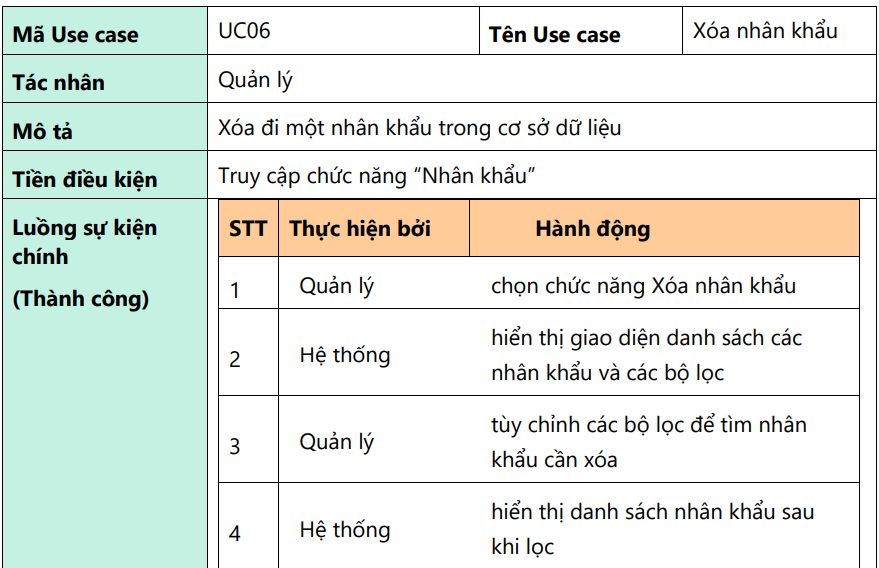
\includegraphics[width=0.8\textwidth]{Ảnh chương 2/UC06 1.png}
    \end{figure}
    \begin{figure}[H]
        \centering
        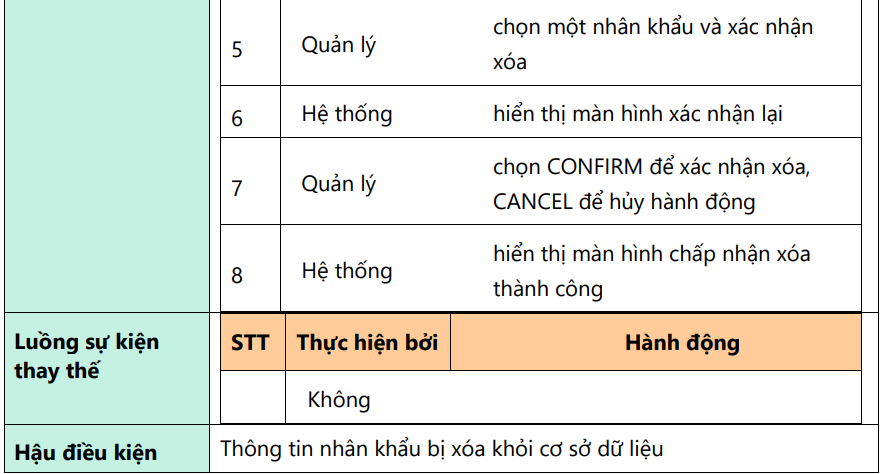
\includegraphics[width=0.8\textwidth]{Ảnh chương 2/UC06.png}
    \end{figure}
    \begin{figure}[H]
        \centering
        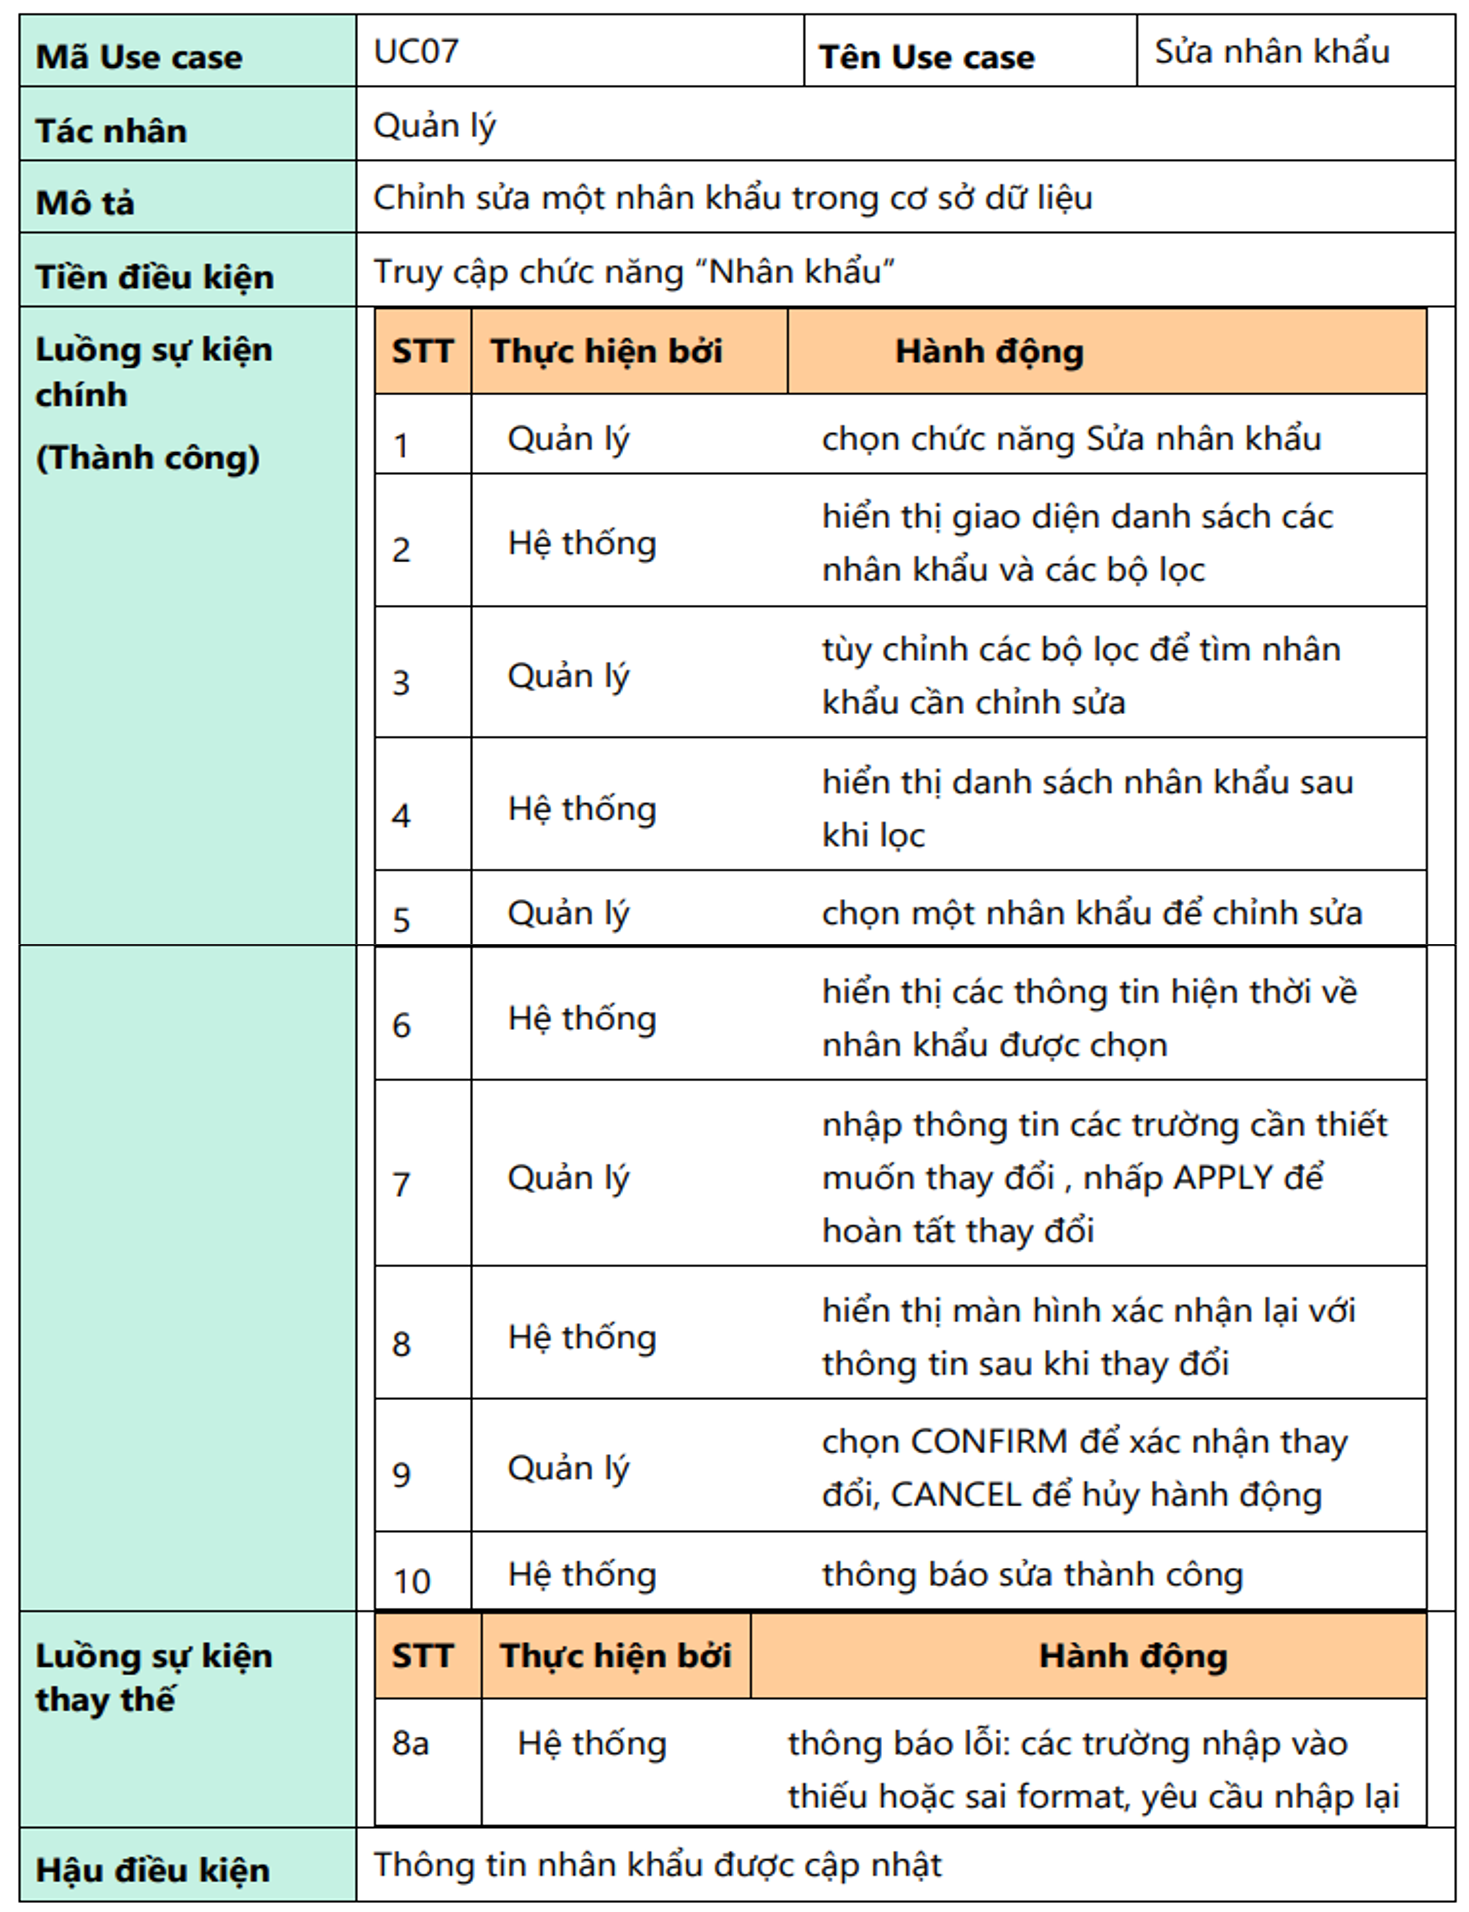
\includegraphics[width=0.8\textwidth]{Ảnh chương 2/UC07.png}
    \end{figure}
    \begin{figure}[H]
        \centering
        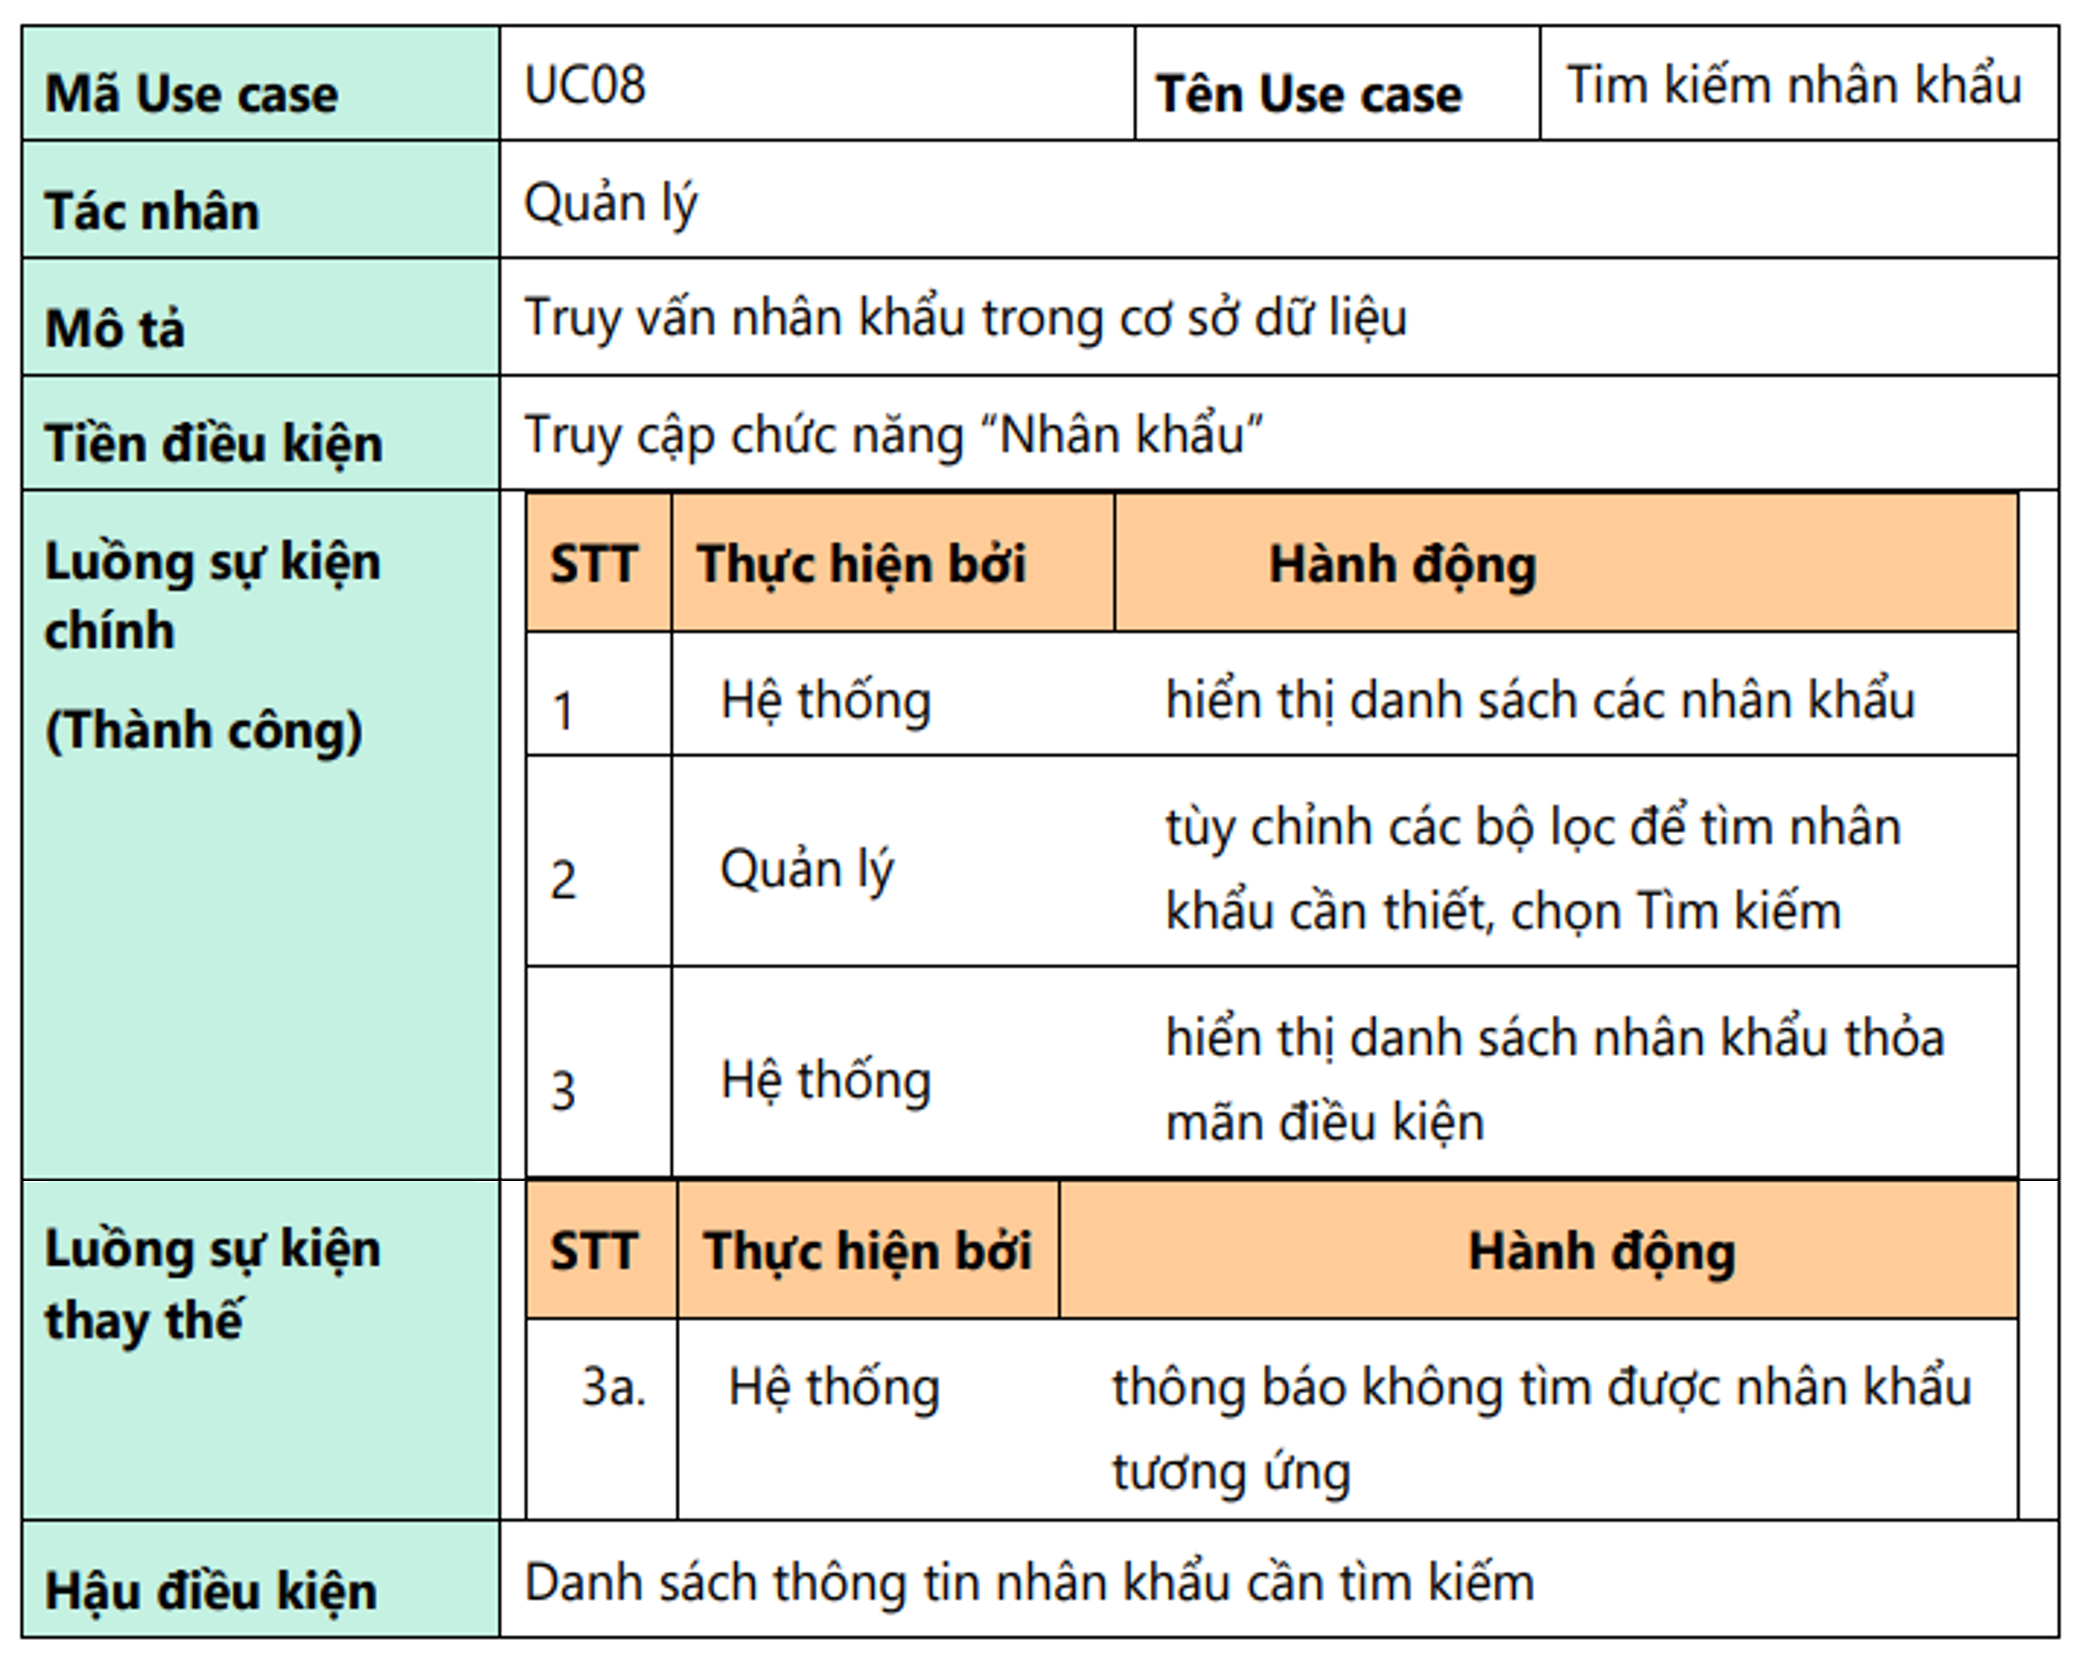
\includegraphics[width=0.8\textwidth]{Ảnh chương 2/UC08.png}
    \end{figure}
    \item Quản lý hộ khẩu
    \begin{figure}[H]
        \centering
        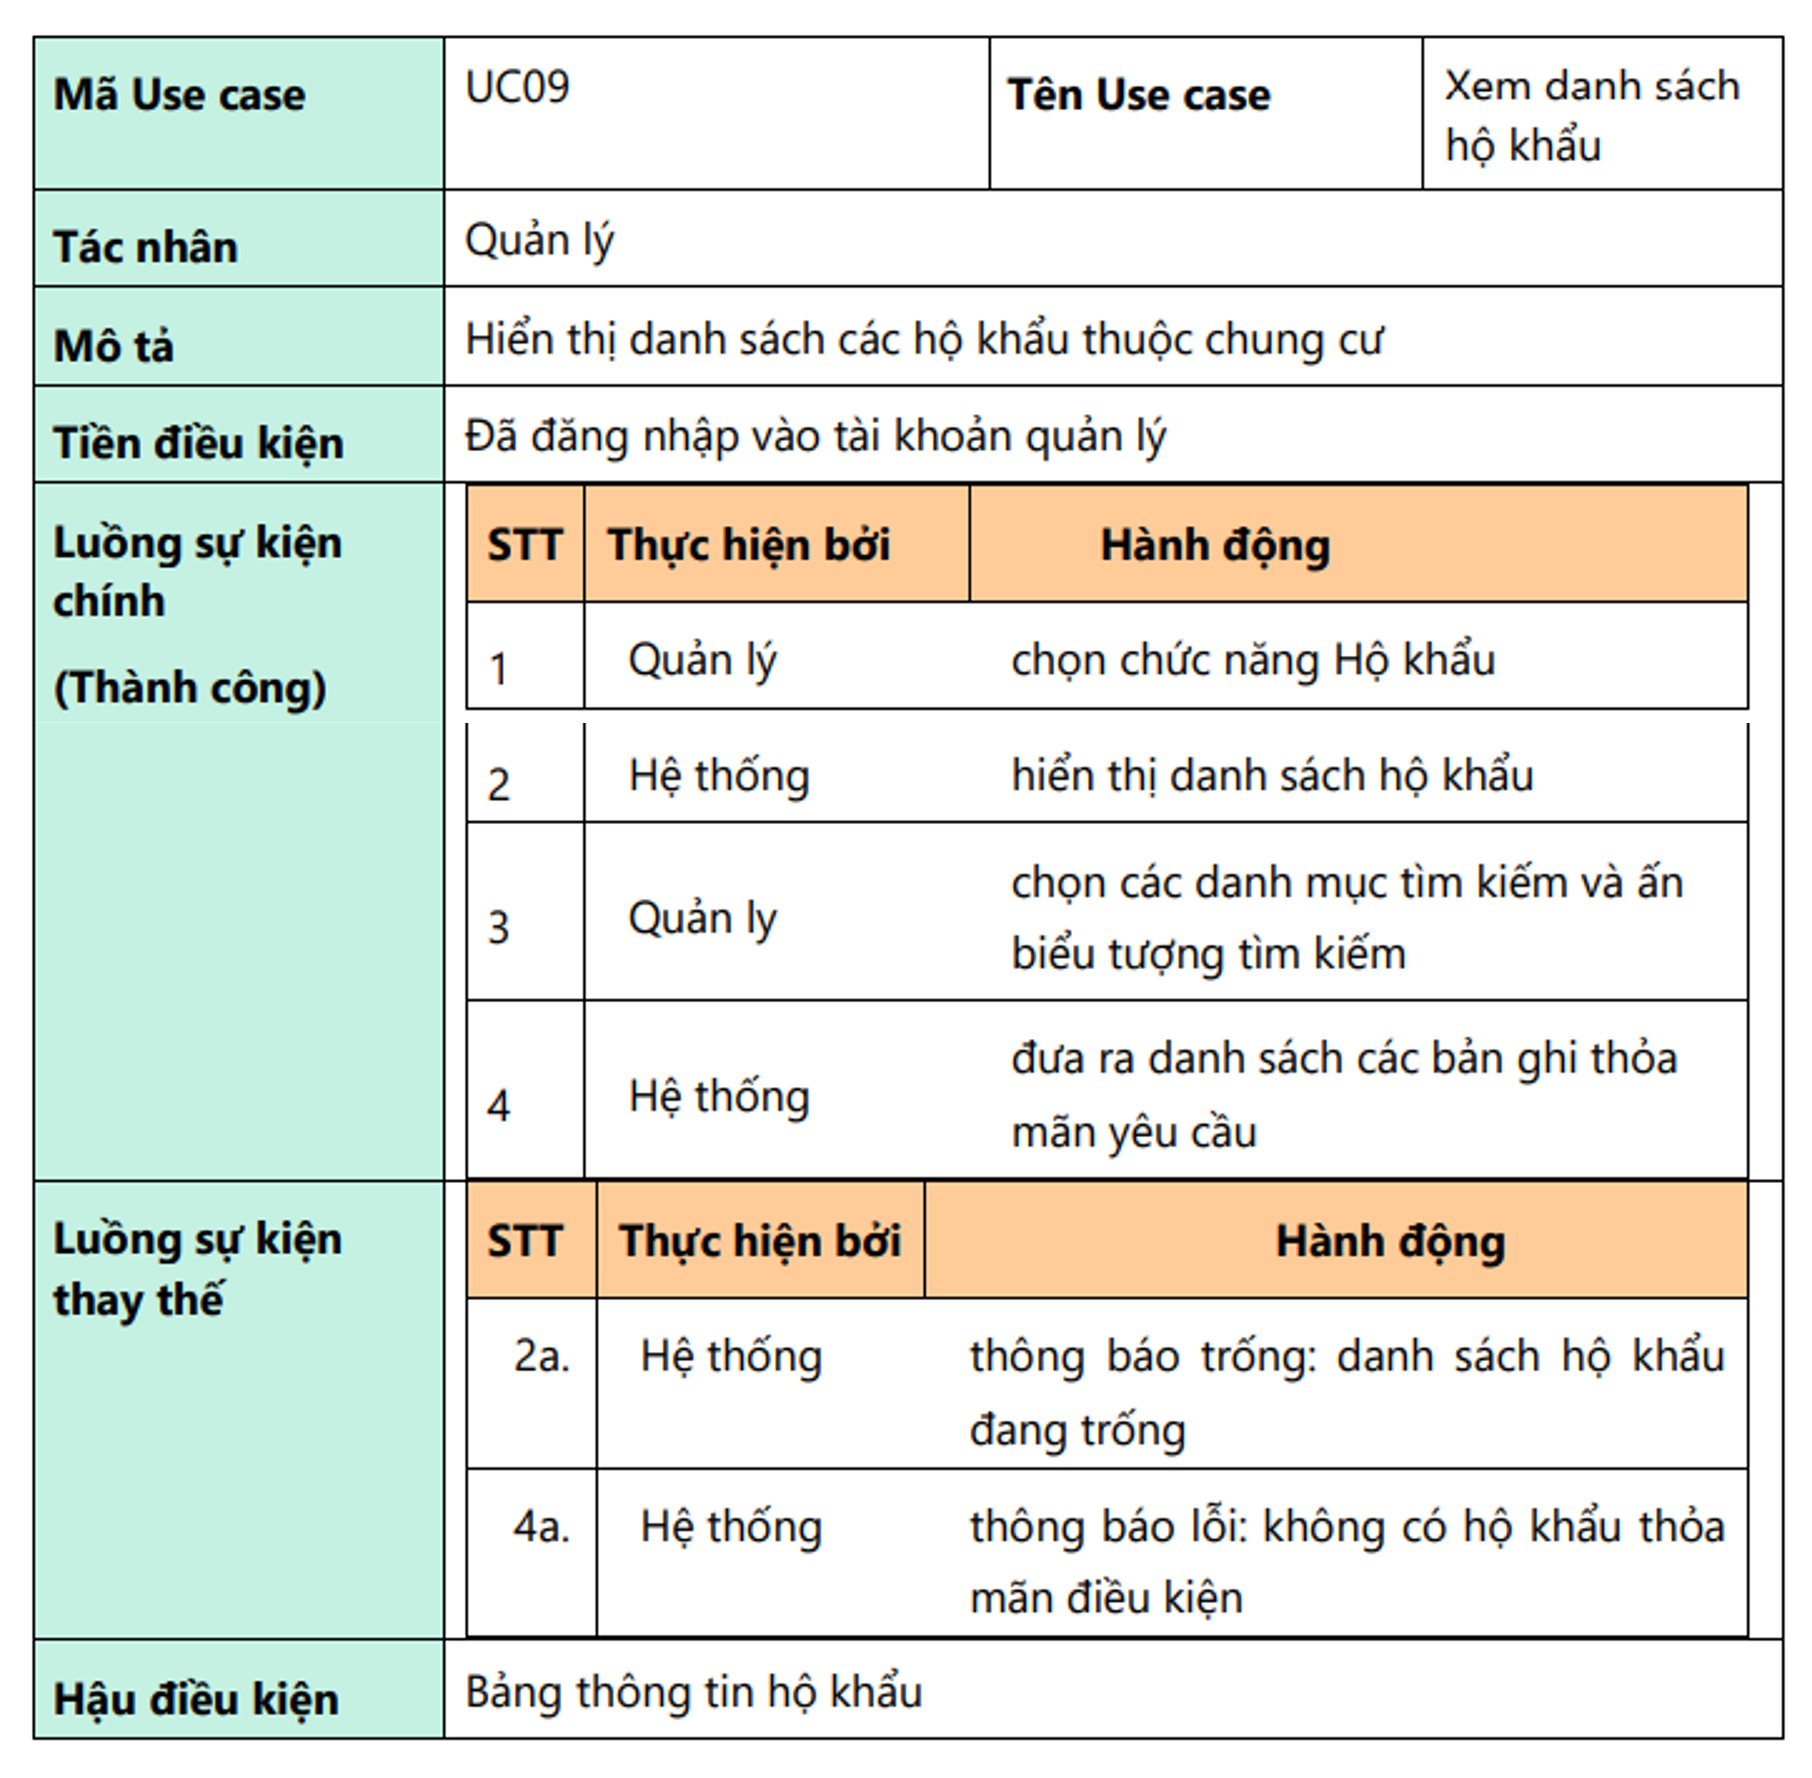
\includegraphics[width=0.8\textwidth]{Ảnh chương 2/UC09.png}
    \end{figure}
    \begin{figure}[H]
        \centering
        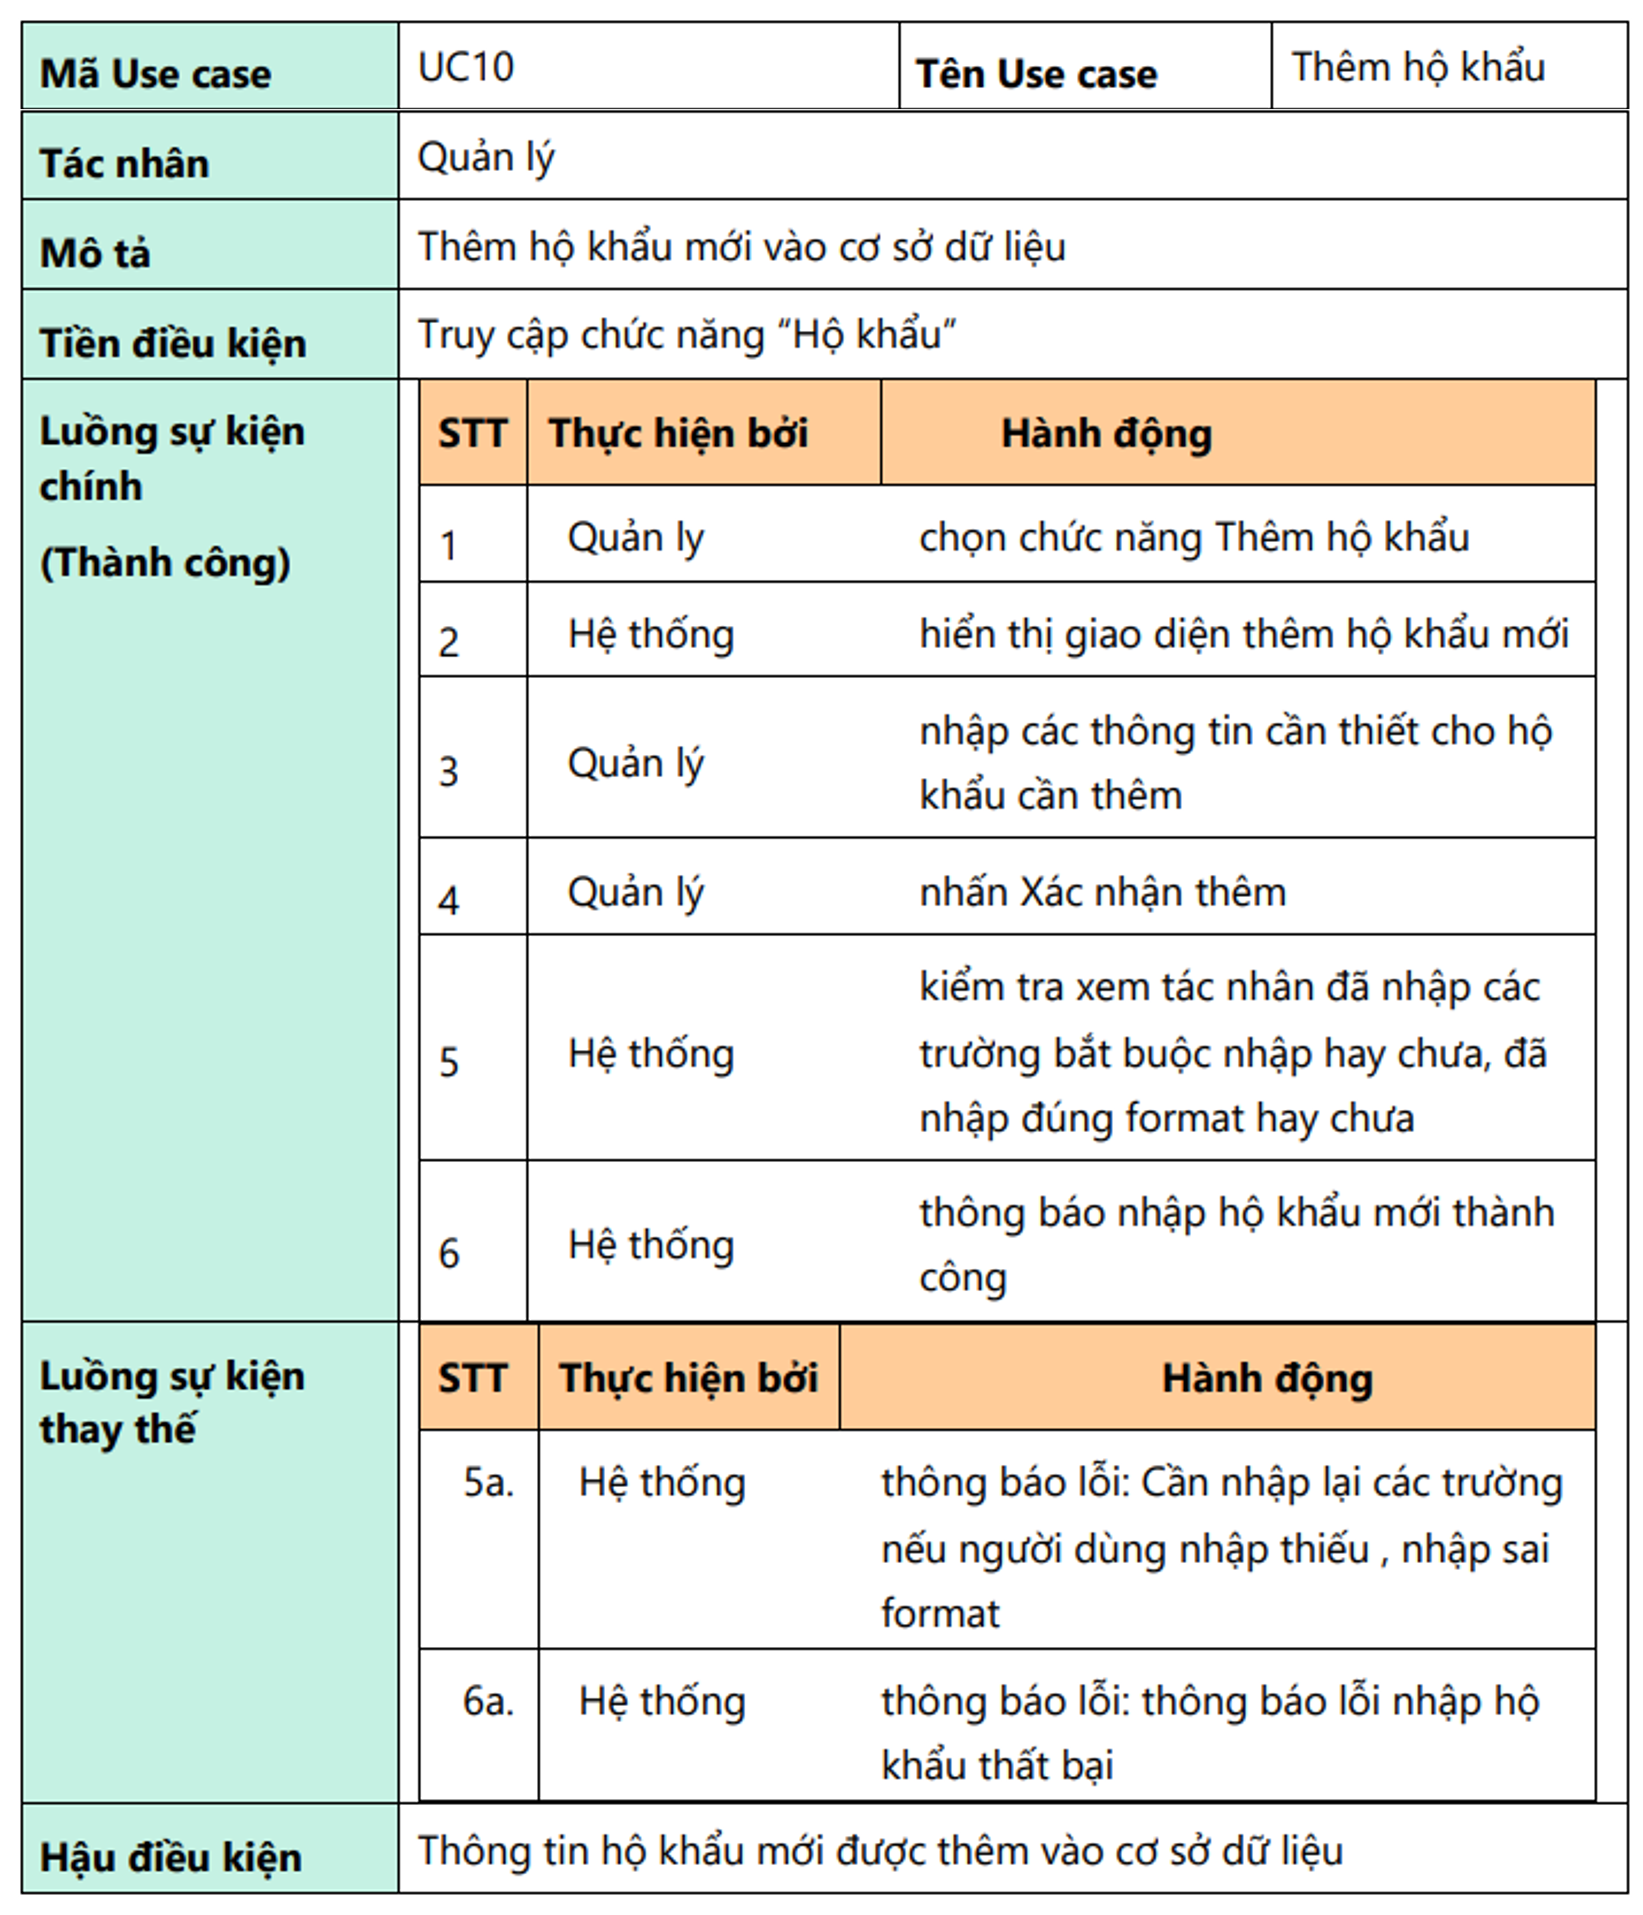
\includegraphics[width=0.8\textwidth]{Ảnh chương 2/UC10.png}
    \end{figure}
        \begin{figure}[H]
        \centering
        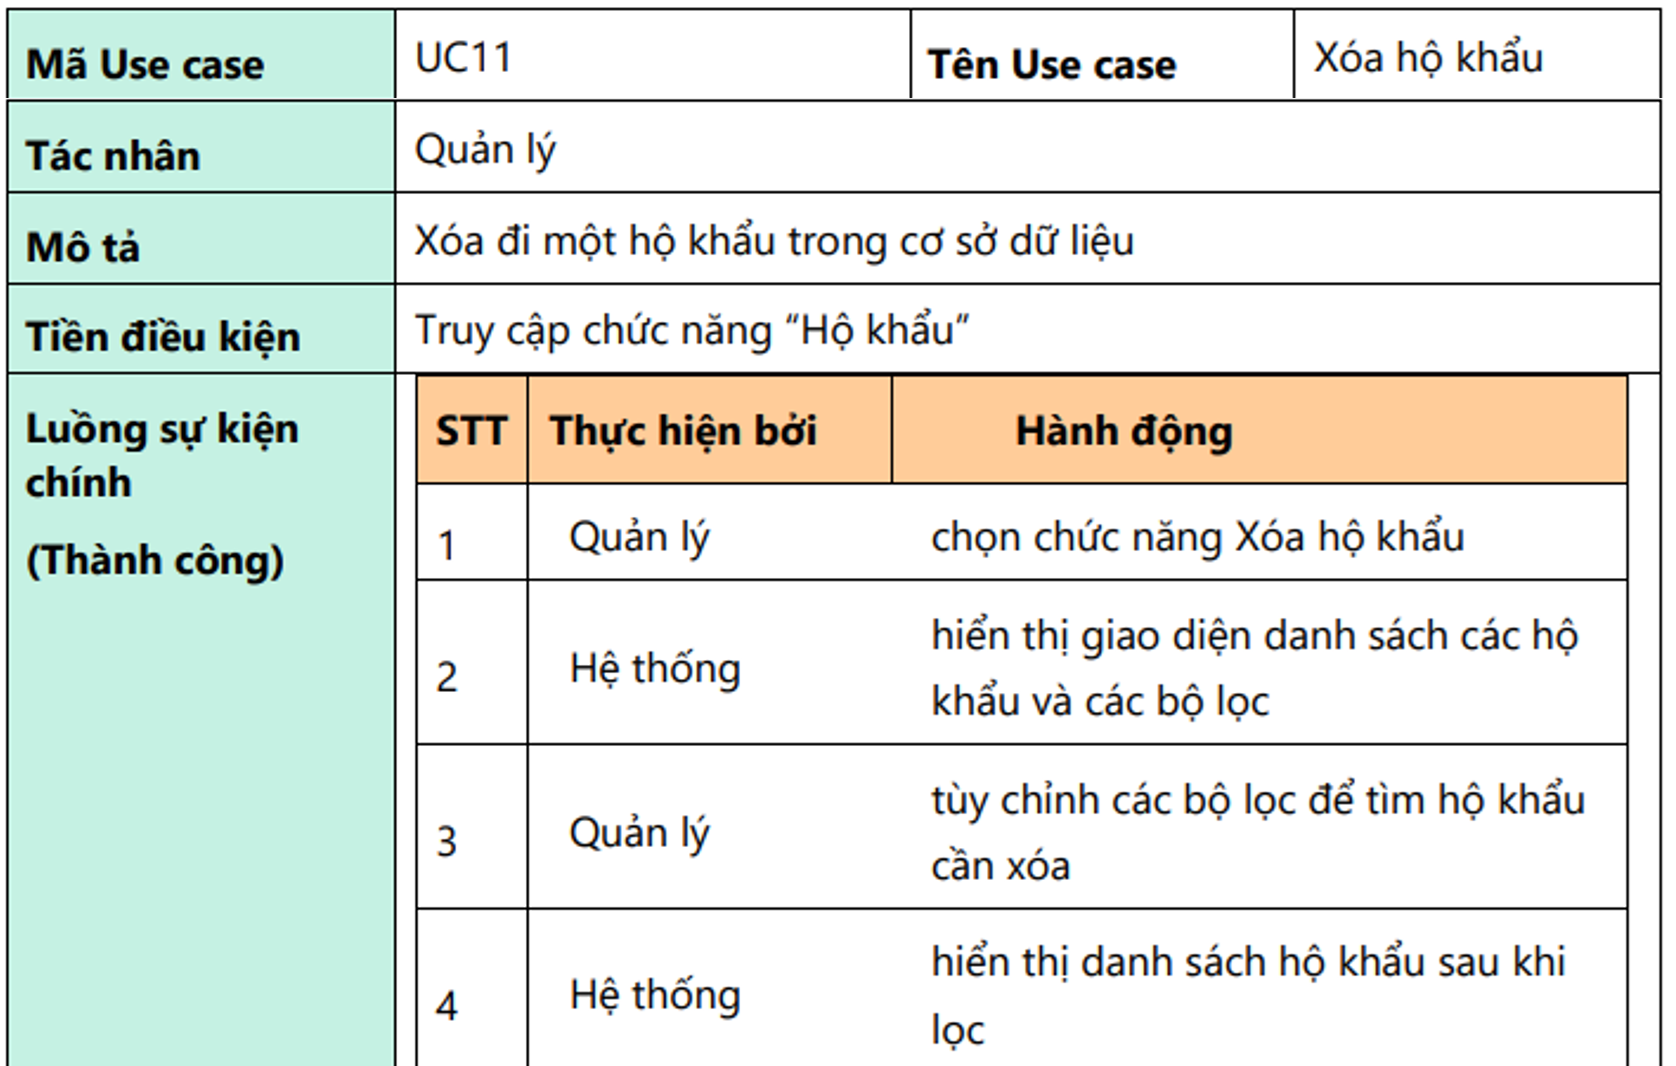
\includegraphics[width=0.8\textwidth]{Ảnh chương 2/UC11 1png.png}
    \end{figure}
    \begin{figure}[H]
        \centering
        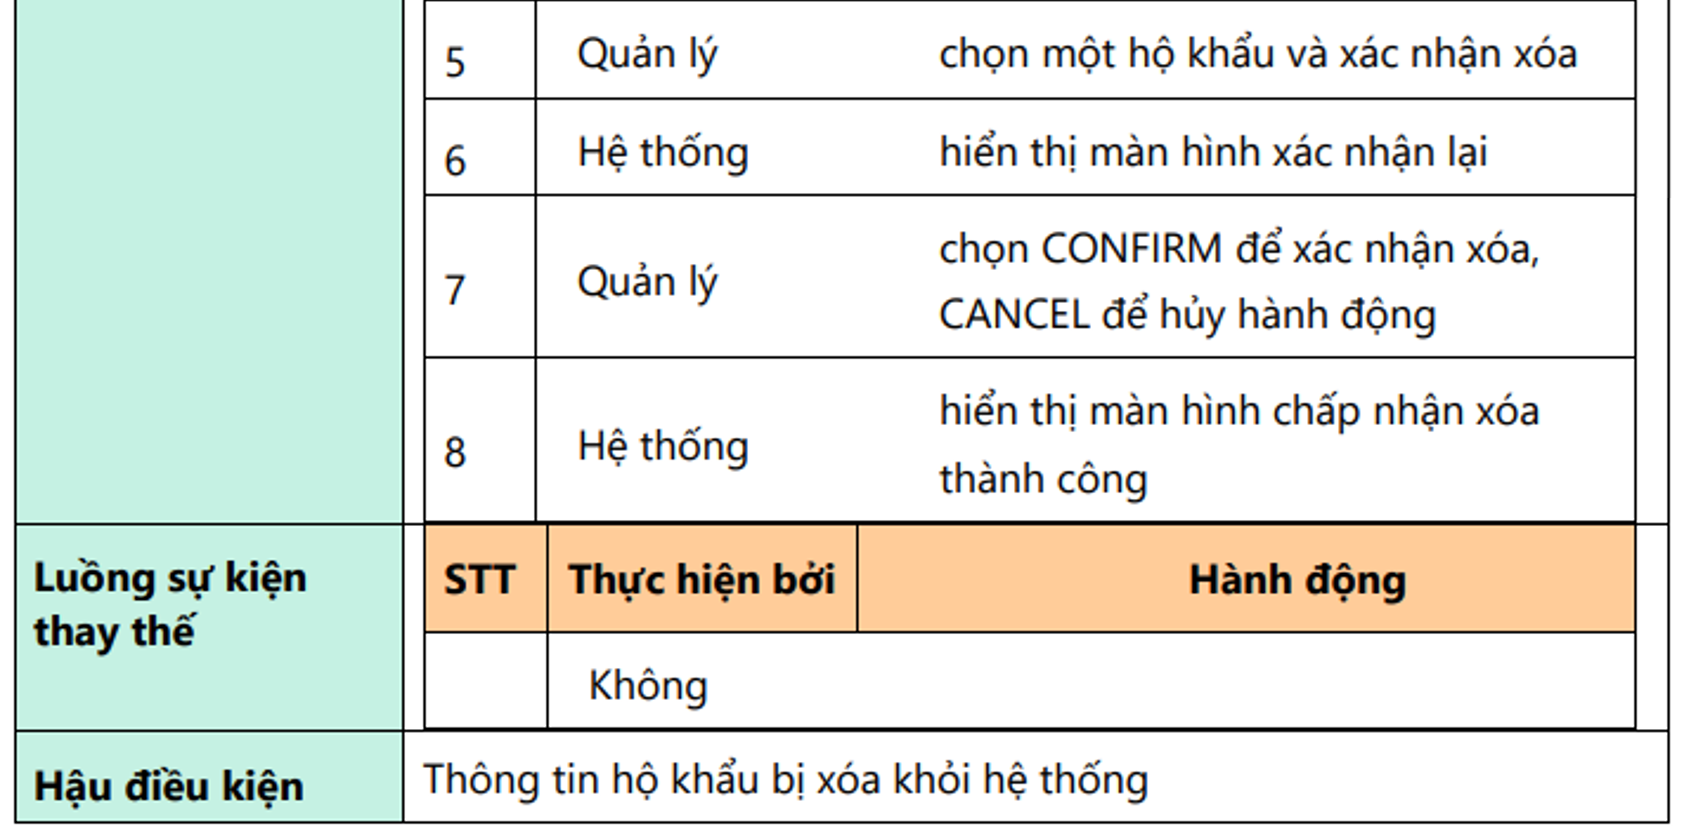
\includegraphics[width=0.8\textwidth]{Ảnh chương 2/UC11.png}
    \end{figure}
    \begin{figure}[H]
        \centering
        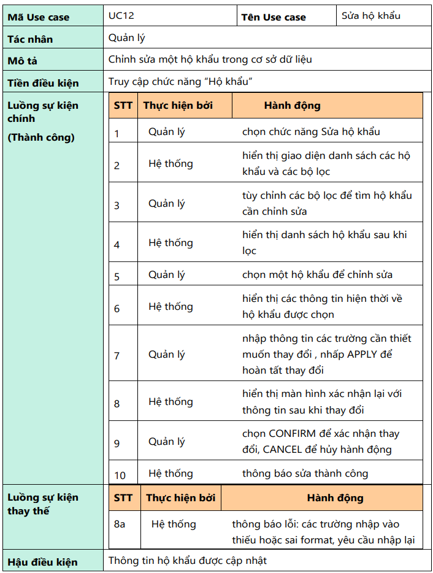
\includegraphics[width=0.8\textwidth]{Ảnh chương 2/UC12.png}
    \end{figure}

    \begin{figure}[H]
        \centering
        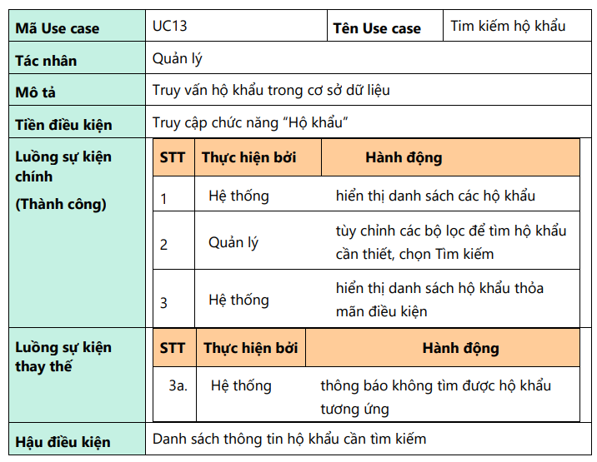
\includegraphics[width=0.8\textwidth]{Ảnh chương 2/UC13.png}
    \end{figure}

    \item Quản lý khoản thu
    \begin{figure}[H]
        \centering
        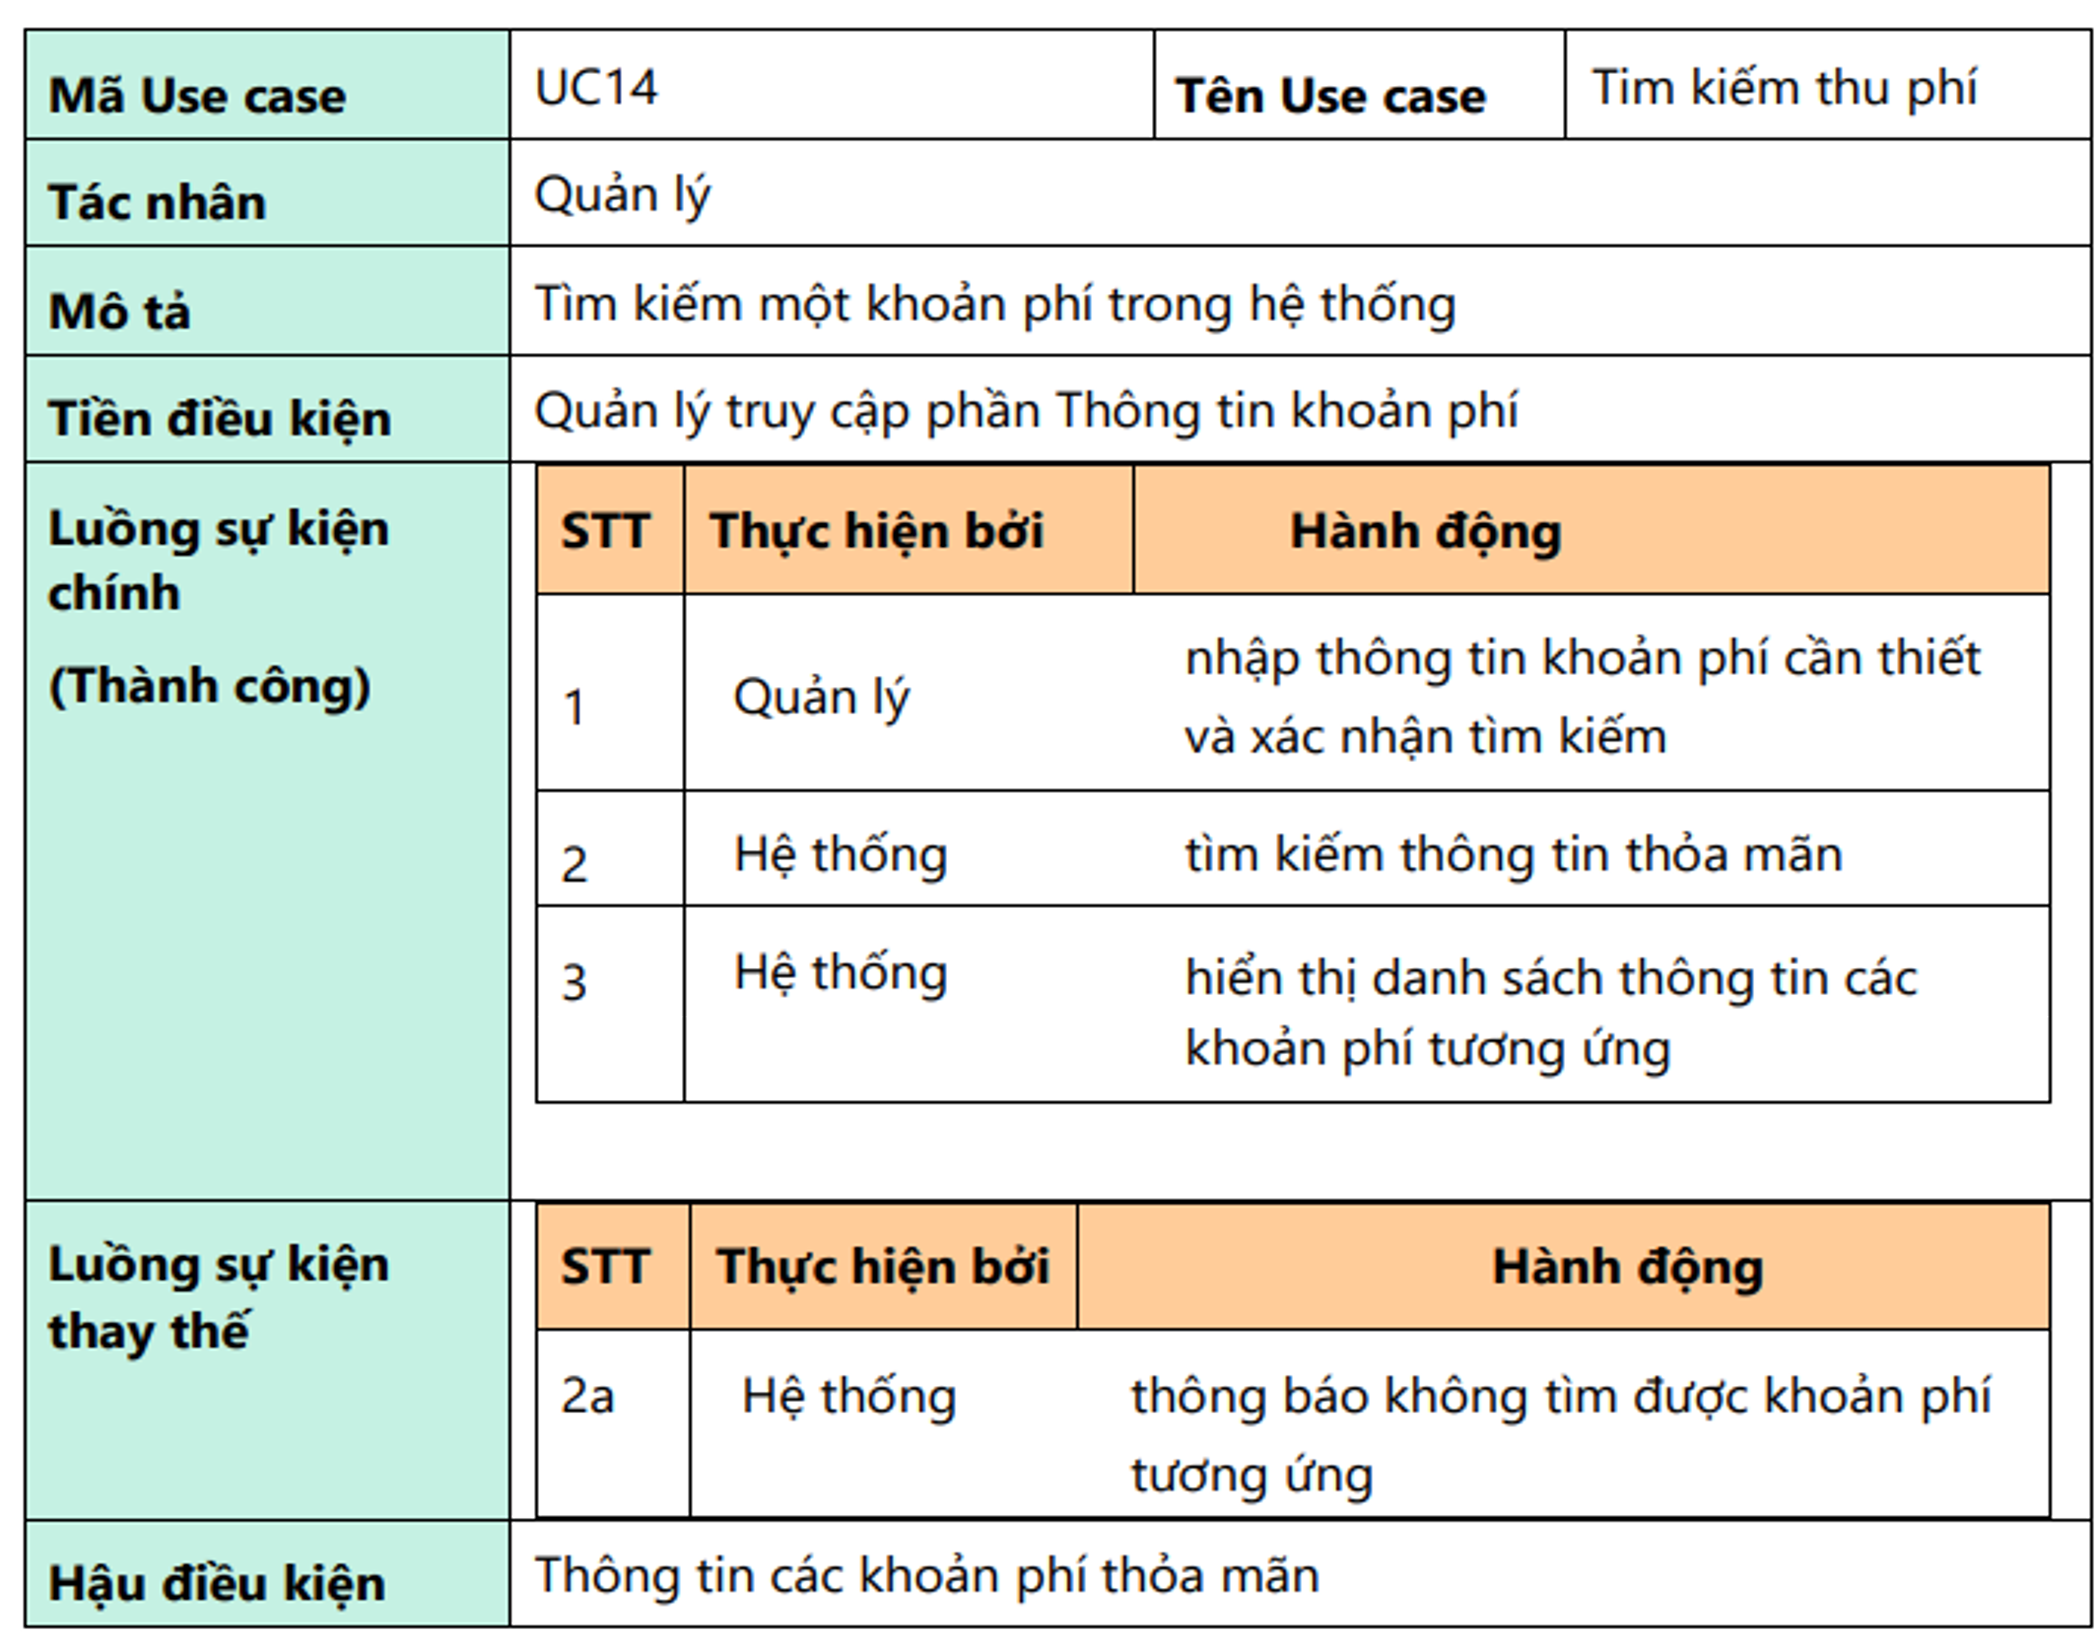
\includegraphics[width=0.8\textwidth]{Ảnh chương 2/UC14.png}
    \end{figure}
    \begin{figure}[H]
        \centering
        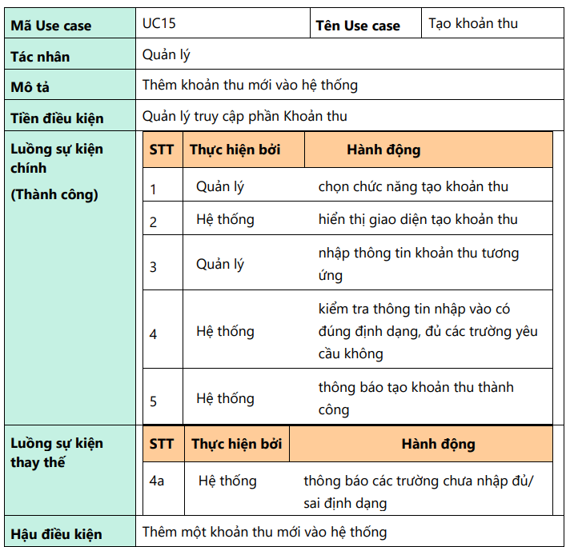
\includegraphics[width=0.8\textwidth]{Ảnh chương 2/UC15.png}
    \end{figure}
    \begin{figure}[H]
        \centering
        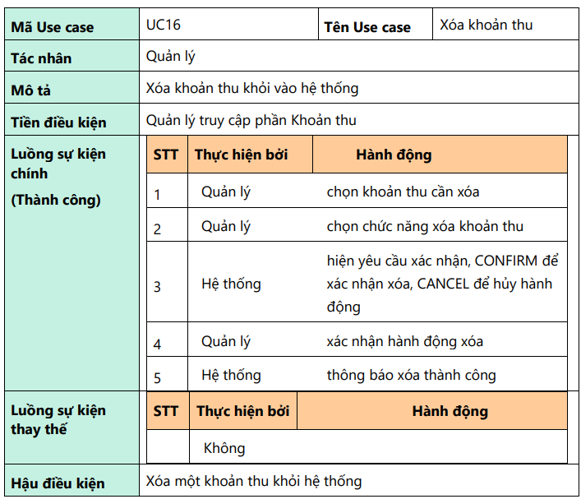
\includegraphics[width=0.8\textwidth]{Ảnh chương 2/UC16.png}
    \end{figure}
    \item Quản lý tài khoản
    \begin{figure}[H]
        \centering
        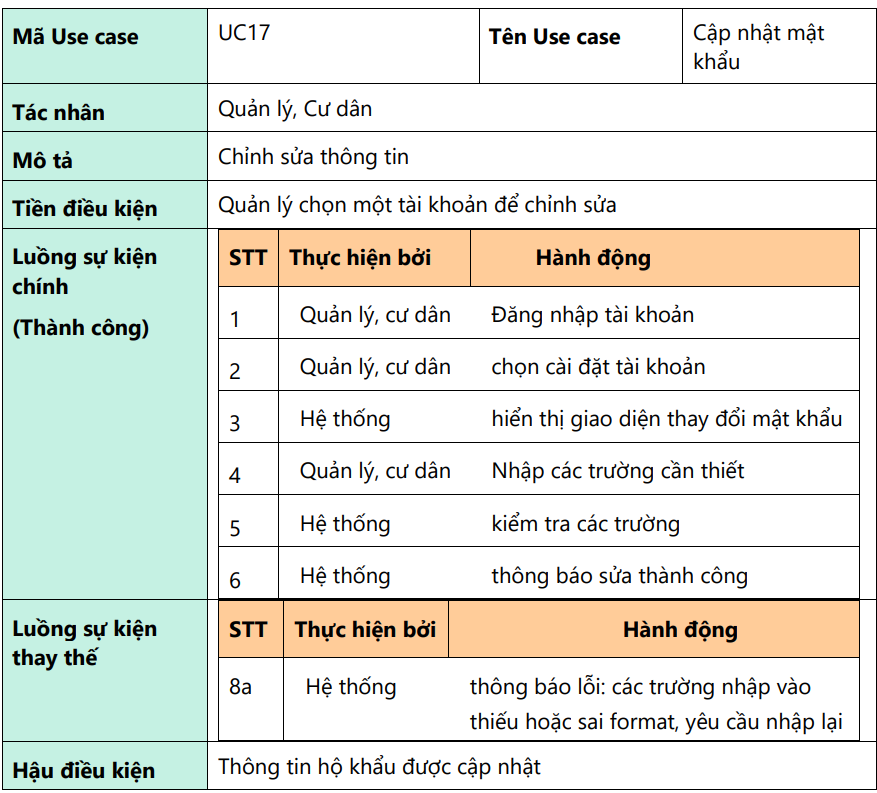
\includegraphics[width=0.8\textwidth]{Ảnh chương 2/UC17.png}
    \end{figure}
    \item Tra cứu thông tin
    \begin{figure}[H]
        \centering
        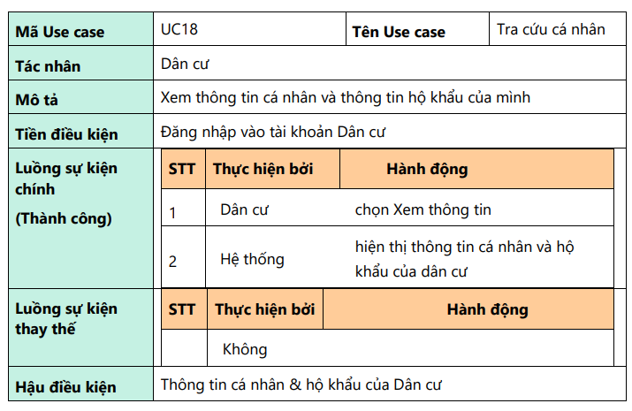
\includegraphics[width=0.8\textwidth]{Ảnh chương 2/UC18.png}
    \end{figure}
\end{itemize}
\vspace{1cm}
\subsection{Các yêu cầu phi chức năng}
Chức năng
\begin{itemize}
    \item Hỗ trợ nhiều quản lý và cư dân truy cập đồng thời
    \item Quản lý thông tin nhân khẩu, hộ khẩu, thông tin thu phí và khoản thu của các hộ dân cư
\end{itemize}

Tính dễ dùng
\begin{itemize}
    \item Giao diện nguời dùng tương thích Windows 7/ Window 10. Thân thiện.
\end{itemize}

Tính ổn định
\begin{itemize}
    \item Hệ thống phải hoạt động liên tục 24 giờ/ngày, 7 ngày/tuần
\end{itemize}

Hiệu suất
\begin{itemize}
    \item Hệ thống phải hỗ trợ đến 1000 người dùng truy xuất CSDL trung tâm đồng thời bất kỳ lúc nào, và đến 500 người dùng truy xuất các server cục bộ. 
    \item Hoàn thành các thao tác nhanh, chuyển giao diện không quá 2s
\end{itemize}

Sự hỗ trợ
\begin{itemize}
    \item Không
\end{itemize}

Các ràng buộc thiết kế
\begin{itemize}
    \item Không
\end{itemize}
\newpage
% % ----------------------------------------------------------------------------
% \section*{CHƯƠNG 3. PHÂN TÍCH YÊU CẦU}
% \addcontentsline{toc}{section}{CHƯƠNG 3. PHÂN TÍCH YÊU CẦU}
% \setcounter{section}{3}
% \setcounter{subsection}{0}
% \subsection{Xác định các lớp phân tích}
% \subsection{Xây dựng biểu đồ trình tự}
% \subsection{Xây dựng biểu đồ lớp phân tích}
% \subsection{Xây dựng biểu đồ thực thể liên kết (ERD)}
% - Xác định các đối tượng dữ liệu: các đối tượng dữ liệu bao gồm nhân khẩu, hộ khẩu, các khoản phí cần nộp

% - Xác định các đặc tính của đối tượng dữ liệu:
% \begin{itemize}[leftmargin = 1.5cm]
%     \item Nhân khẩu: Định danh nhân khẩu, số CCCD, tuổi nhân khẩu, tên nhân khẩu, quan hệ với chủ hộ
%     \item Hộ khẩu: Mã hộ (Định danh hộ khẩu), số thành viên trong hộ khẩu, địa chỉ của hộ khẩu, thông tin về chủ hộ
%     \item Khoản phí: Mã khoản phí (định danh khoản phí), số tiền, loại khoản phí, tên khoản phí, thời gian nộp, trạng thái nộp đủ chưa
% \end{itemize}

% - Các mối quan hệ giữa các đối tượng dữ liệu : 
% \begin{itemize}[leftmargin = 1.5cm]
%     \item Hộ khẩu sẽ chứa nhiều nhân khẩu hay 1 nhân khẩu sẽ thuộc (nằm trong) 1 hộ khẩu.
%     \item Nhân khẩu là chủ hộ của hộ khẩu.
%     \item Khoản nộp là sự hợp thành từ 1 khoản thu và 1 hộ khẩu. 
% \end{itemize}

% - Biểu đồ ERD mô tả mối quan hệ giữa các đối tượng dữ liệu:
% \newpage 

% %---------------------------------------------------------------------
\section*{CHƯƠNG 4. THIẾT KẾ CHƯƠNG TRÌNH}
\addcontentsline{toc}{section}{CHƯƠNG 4. THIẾT KẾ CHƯƠNG TRÌNH}
\setcounter{section}{4}
\setcounter{subsection}{0}

% \subsection{Thiết kế kiến trúc}
% Viết kiến trúc vào đây

% \subsection{Thiết kế cơ sở dữ liệu}
% Sơ đồ quan hệ giữa các bảng:

% \describetable{Đặc tả dữ liệu cho bảng nhân khẩu:}
% {
%     \addRow\getRowWithColor{\textbf{\underline{ID}}}{int}{}{Khoá chính}{Số nguyên \newline dương}{}{white}
%     \addRow\getRowWithColor{username}{Varchar(60)}{60 ký tự}{not null}{Văn bản}{}{lightblue}
%     \addRow\getRowWithColor{\textbf{\underline{ID}}}{int}{}{Khoá chính}{Số nguyên \newline dương}{}{white}
%     \addRow\getRowWithColor{username}{Varchar(60)}{60 ký tự}{not null}{Văn bản}{}{lightblue}
% }

% \describetable{Đặc tả dữ liệu cho bảng tài khoản:}
% {
%     \addRow\getRowWithColor{\textbf{\underline{ID}}}{int}{}{Khoá chính}{Số nguyên \newline dương}{}{white}
%     \addRow\getRowWithColor{username}{Varchar(60)}{60 ký tự}{not null}{Văn bản}{}{lightblue}
% }

% \describetable{Đặc tả dữ liệu cho bảng tài khoản:}
% {
%     \addRow\getRowWithColor{\textbf{\underline{ID}}}{int}{}{Khoá chính}{Số nguyên \newline dương}{}{white}
%     \addRow\getRowWithColor{username}{Varchar(60)}{60 ký tự}{not null}{Văn bản}{}{lightblue}
% }

% \describetable{Đặc tả dữ liệu cho bảng tài khoản:}
% {
%     \addRow\getRowWithColor{\textbf{\underline{ID}}}{int}{}{Khoá chính}{Số nguyên \newline dương}{}{white}
%     \addRow\getRowWithColor{username}{Varchar(60)}{60 ký tự}{not null}{Văn bản}{}{lightblue}
% }

% \describetable{Đặc tả dữ liệu cho bảng tài khoản:}
% {
%     \addRow\getRowWithColor{\textbf{\underline{ID}}}{int}{}{Khoá chính}{Số nguyên \newline dương}{}{white}
%     \addRow\getRowWithColor{username}{Varchar(60)}{60 ký tự}{not null}{Văn bản}{}{lightblue}
% }
% \newpage

% %--------------------------------------------------------------------------

% \subsection{Thiết kế chi tiết các gói}

% \getpack{Biểu đồ package cho gói Controller:}{0.9}{image/Package/Controller.png}
% \getpack{Biểu đồ package cho gói Model:}{0.8}{image/Package/Model.png}
% \getpack{Biểu đồ package cho gói Service:}{0.9}{image/Package/Service.png}
% \getpack{Biểu đồ package cho gói Repository:}{0.8}{image/Package/Repository.png}
% \newpage
% \getpack{Biểu đồ package cho gói Exception:}{0.7}{image/Package/Exception.png}
% \getpack{Biểu đồ package cho gói DTO:}{0.7}{image/Package/DTO.png}
% \getpack{Biểu đồ package cho gói Config:}{0.7}{image/Package/Config.png}

% \subsection{Thiết kế chi tiết lớp}

% % \begin{tabular}{|l|l|}
% %     \hline
% %     \multicolumn{2}{c}{Class User}  \\
% %      Chứa các thông tin về nhân khẩu \newline 
% %       & 
% % \end{tabular}

% \subsection{Sơ đồ lớp chi tiết}
\subsection{Thiết kế giao diện}
\textbf{Thiết kế mock-up cho từng giao diện của bài toán}
\begin{itemize}
    \item Mock-up cho giao diện đăng nhập của bài toán :
    \begin{figure}[H]
        \centering
        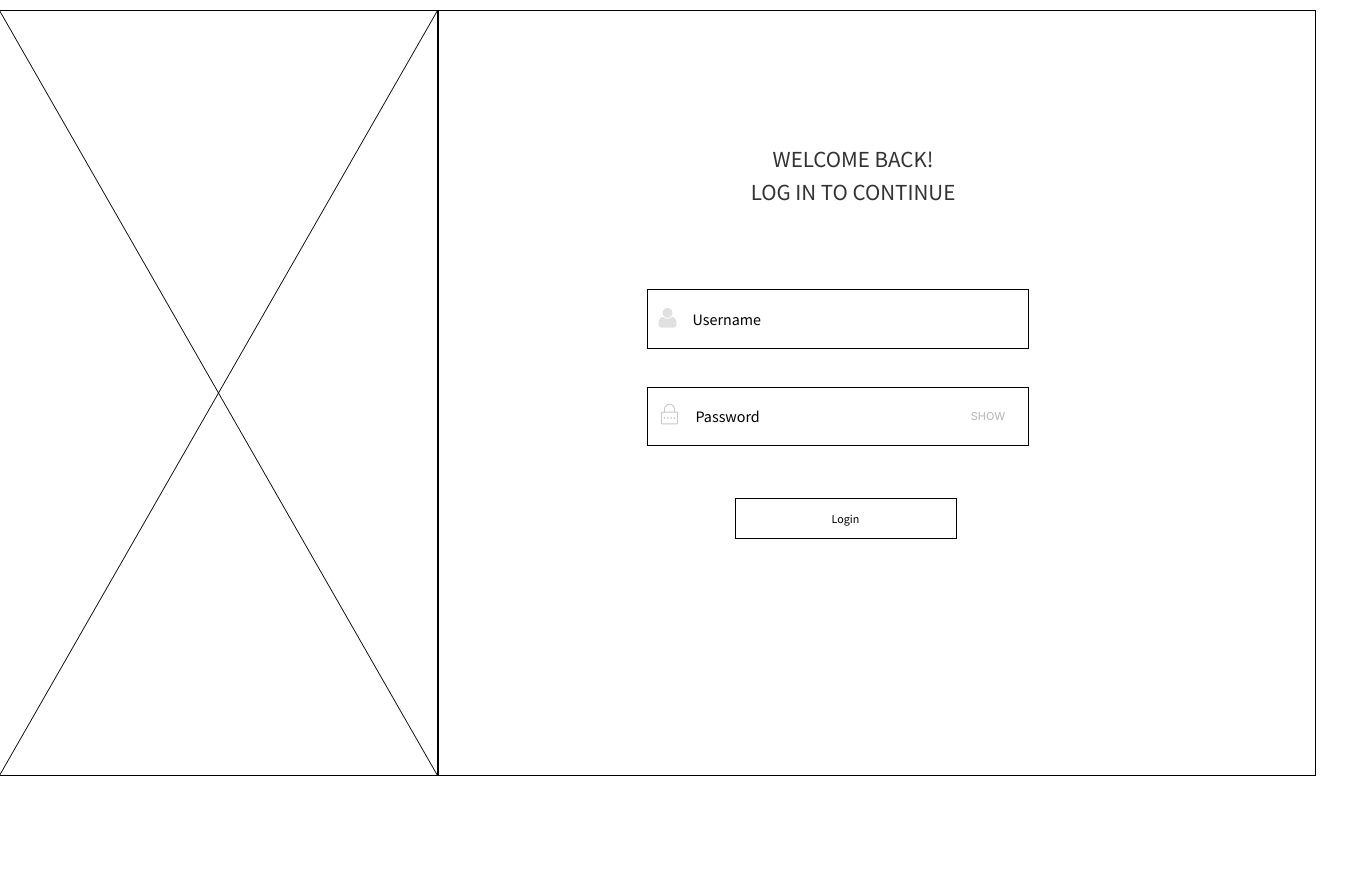
\includegraphics[width=0.8\textwidth]{Ảnh chương 4/Đăng nhập.png}
    \end{figure}
    \item Mock-up cho màn hình chính của bài toán :
    \begin{figure}[H]
        \centering
        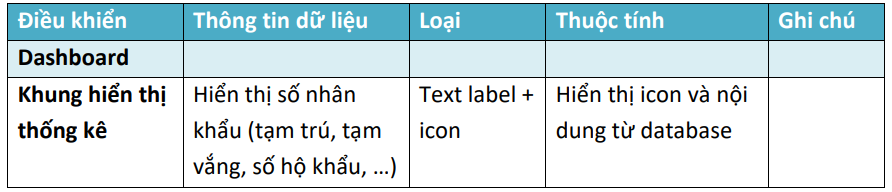
\includegraphics[width=0.8\textwidth]{Ảnh chương 4/Màn hình chính.png}
    \end{figure}
    \vspace{1cm}
    \item Mock-up cho màn hình hộ khẩu của bài toán (Admin):
    \begin{figure}[H]
        \centering
        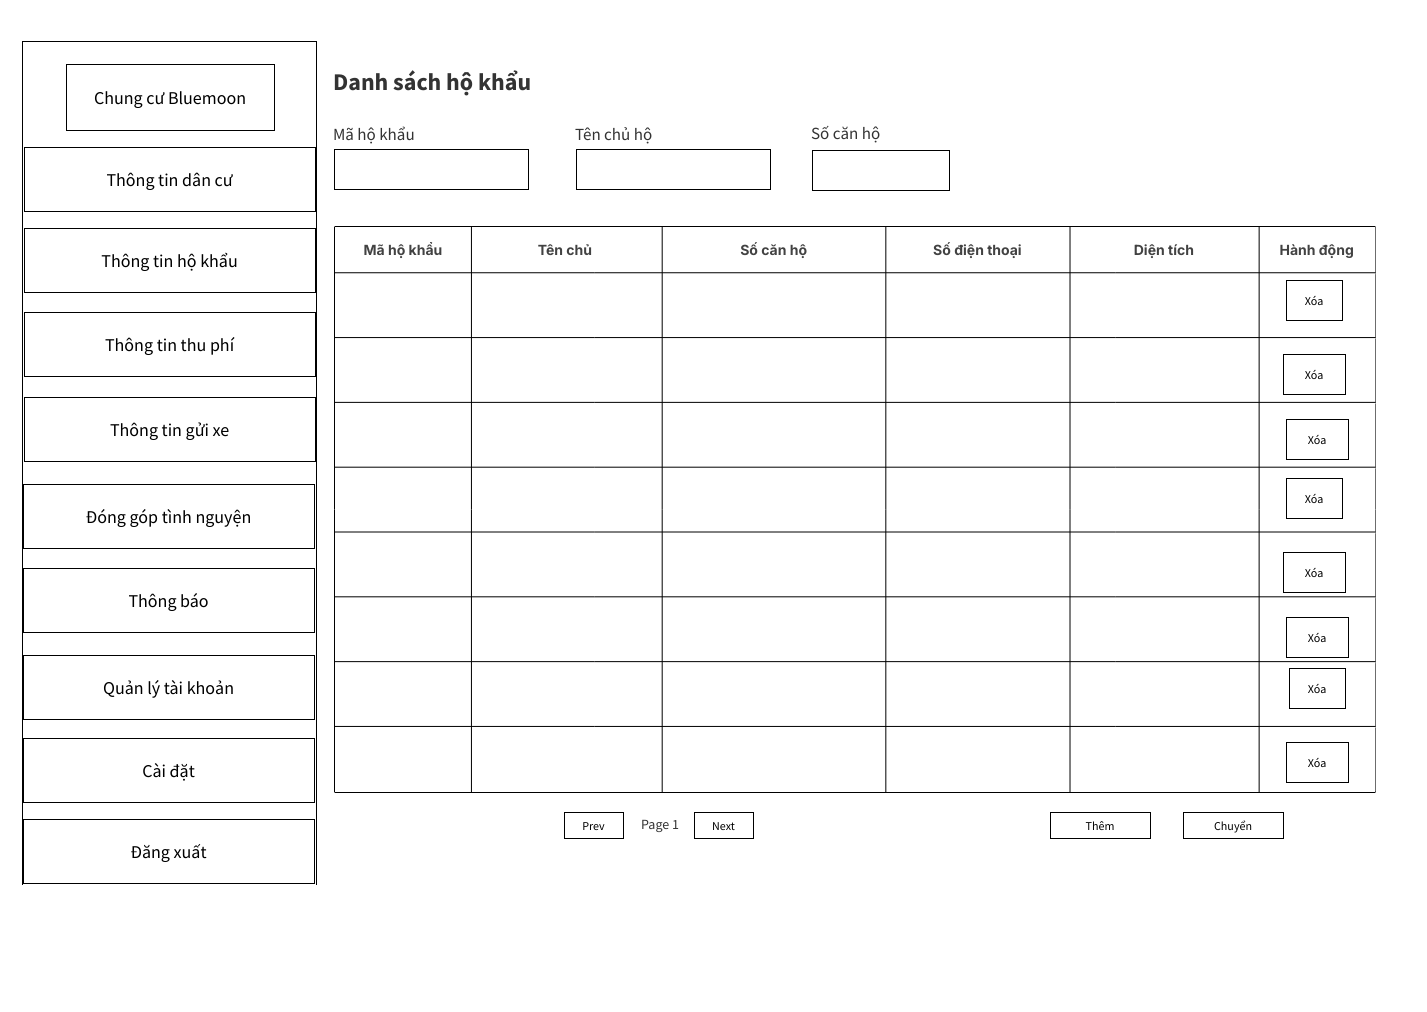
\includegraphics[width=0.8\textwidth]{Ảnh chương 4/Màn hình hộ khẩu.png}
    \end{figure}
    \item Mock-up cho màn hình hộ khẩu của bài toán (User):
    \begin{figure}[H]
        \centering
        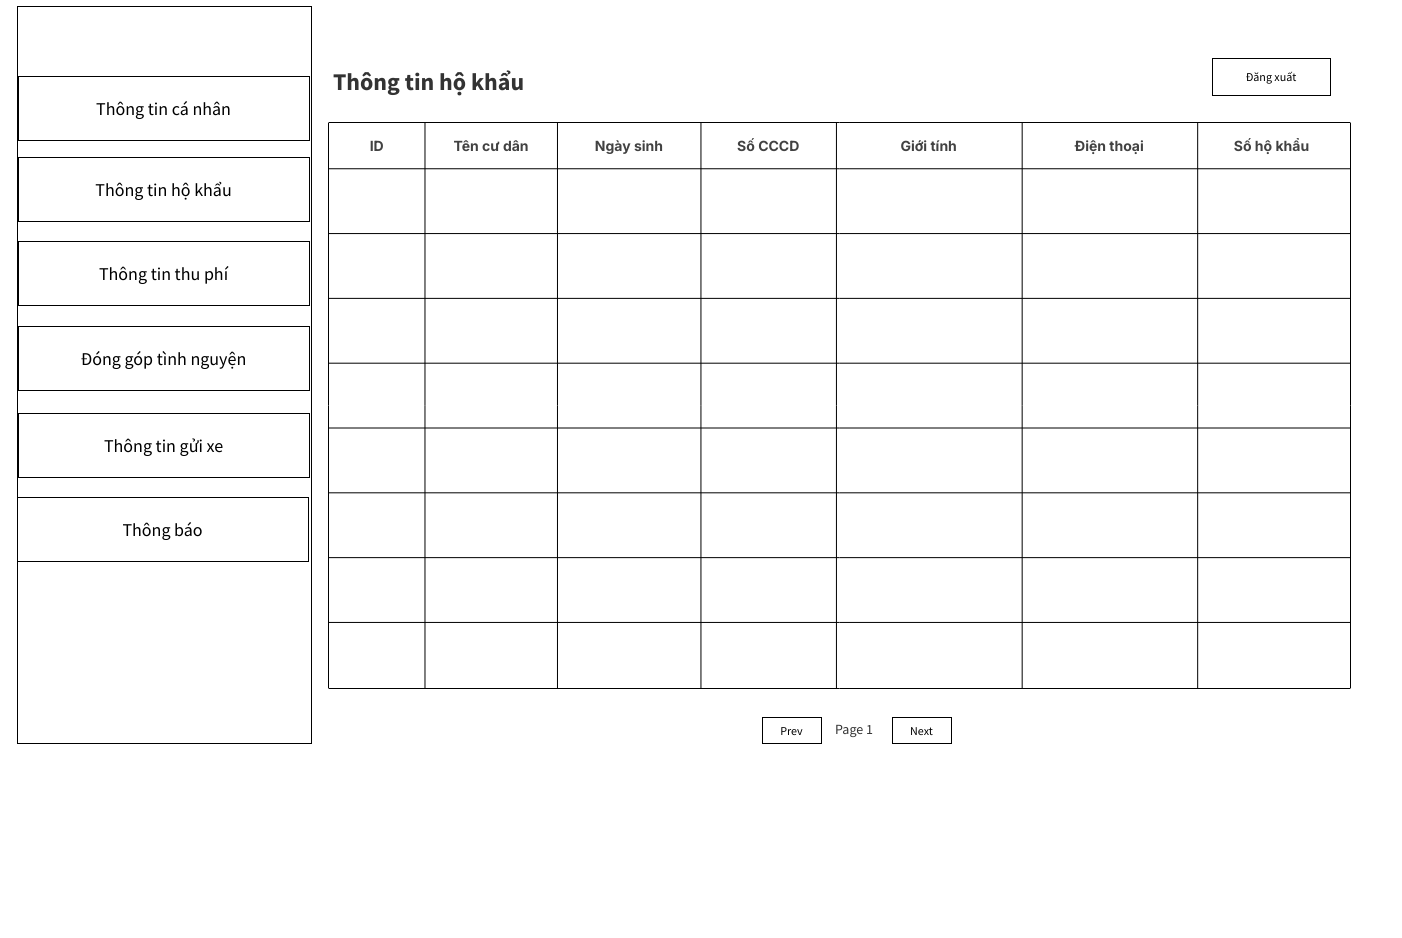
\includegraphics[width=0.8\textwidth]{Ảnh chương 4/Màn hình hộ khẩu (cư dân).png}
    \end{figure}
    \vspace{4cm}
    \item Mock-up cho màn hình xem thông tin chi tiết hộ khẩu của bài toán (Admin):
    \begin{figure}[H]
        \centering
        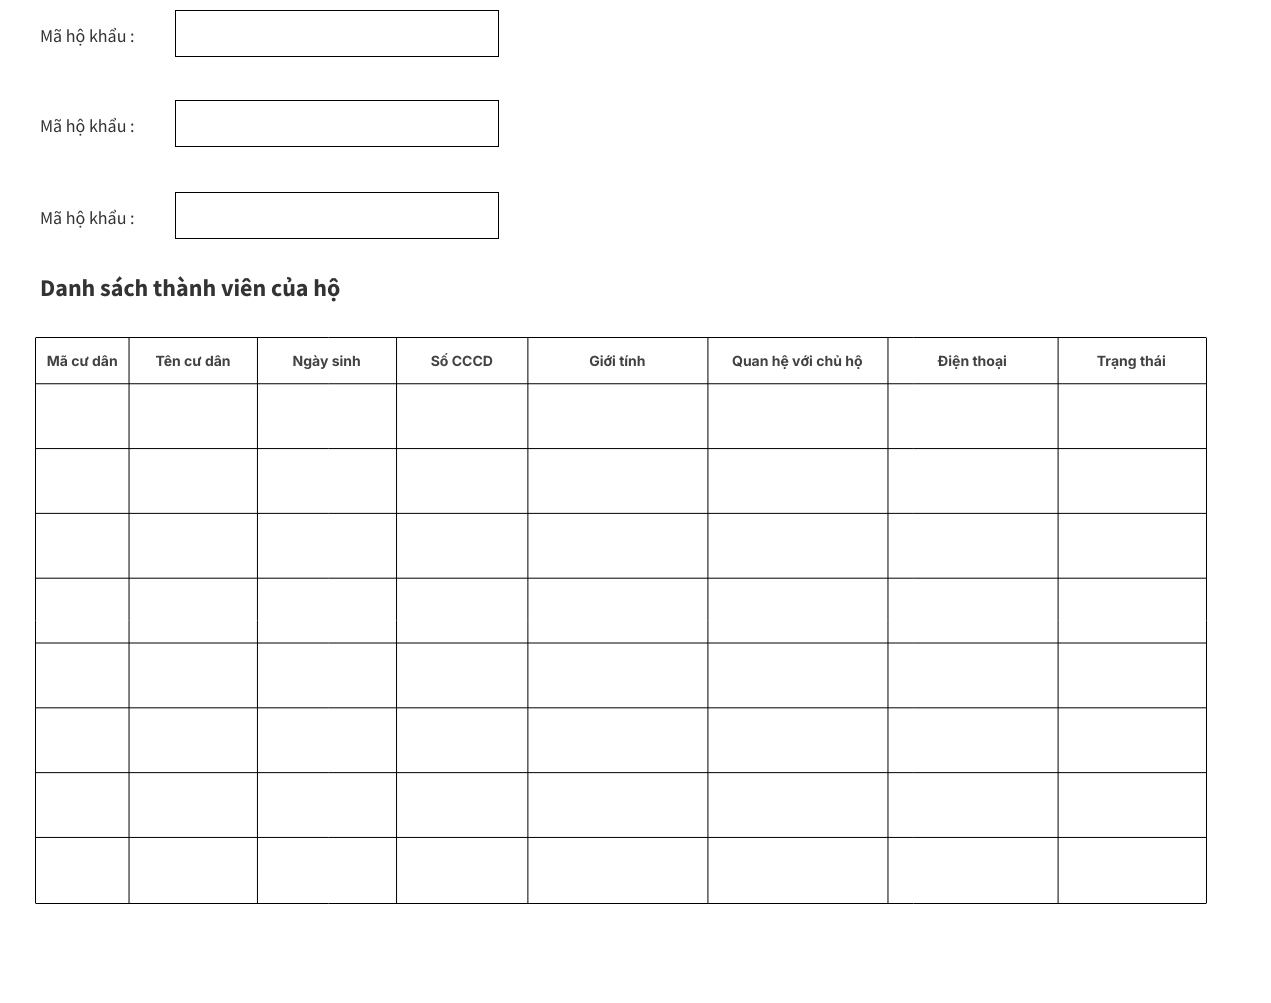
\includegraphics[width=0.75\textwidth]{Ảnh chương 4/Màn hình thông tin hộ khẩu (admin).png}
    \end{figure}
    \item Mock-up cho màn hình thêm hộ khẩu của bài toán (Admin):
    \begin{figure}[H]
        \centering
        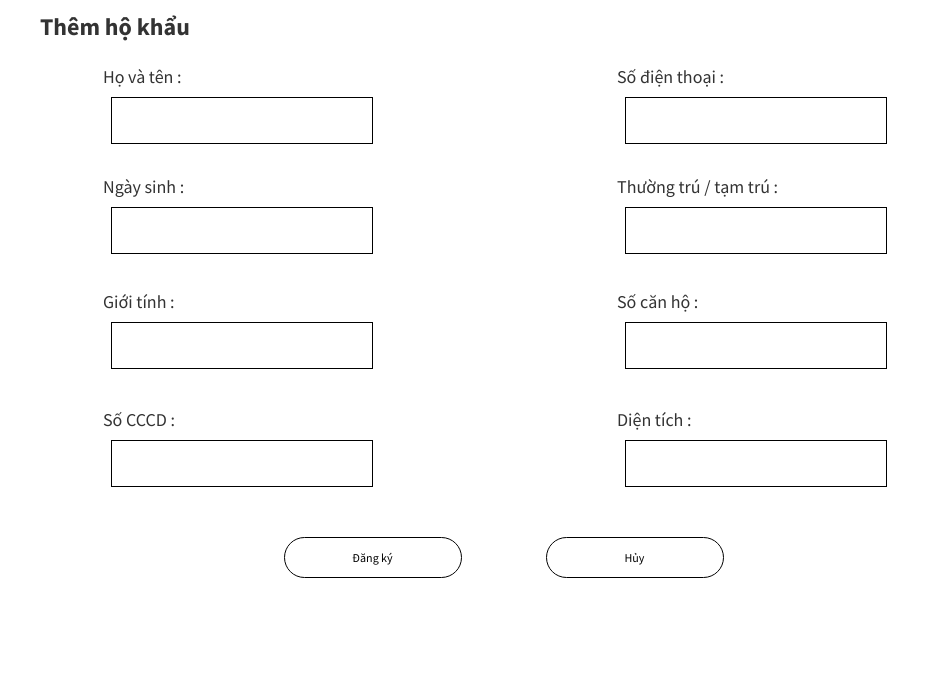
\includegraphics[width=0.75\textwidth]{Ảnh chương 4/Màn hình thêm hộ khẩu.png}
    \end{figure}
    \item Mock-up cho màn hình chuyển hộ khẩu của bài toán (Admin):
    \begin{figure}[H]
        \centering
        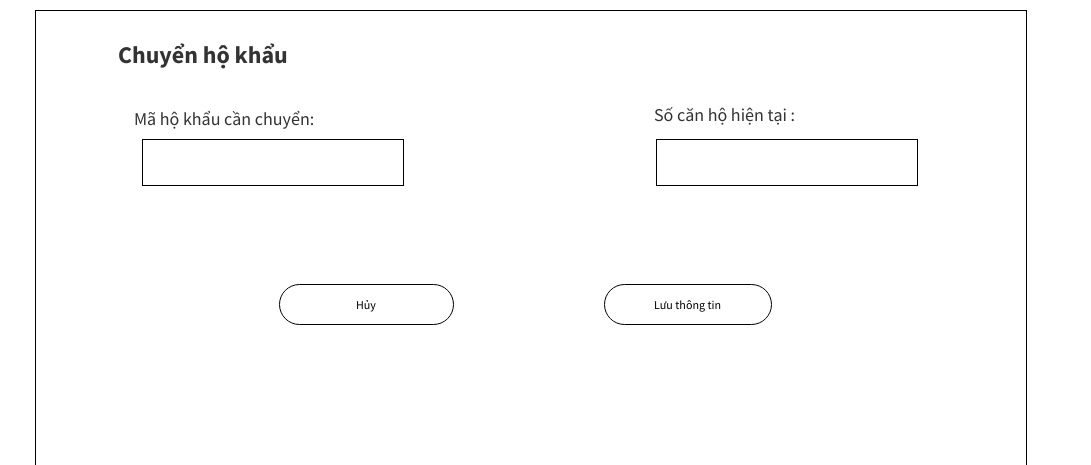
\includegraphics[width=0.9\textwidth]{Ảnh chương 4/Màn hình chuyển hộ khẩu.png}
    \end{figure}
    \vspace{3cm}
    \item Mock-up cho màn hình nhân khẩu của bài toán (Admin):
    \begin{figure}[H]
        \centering
        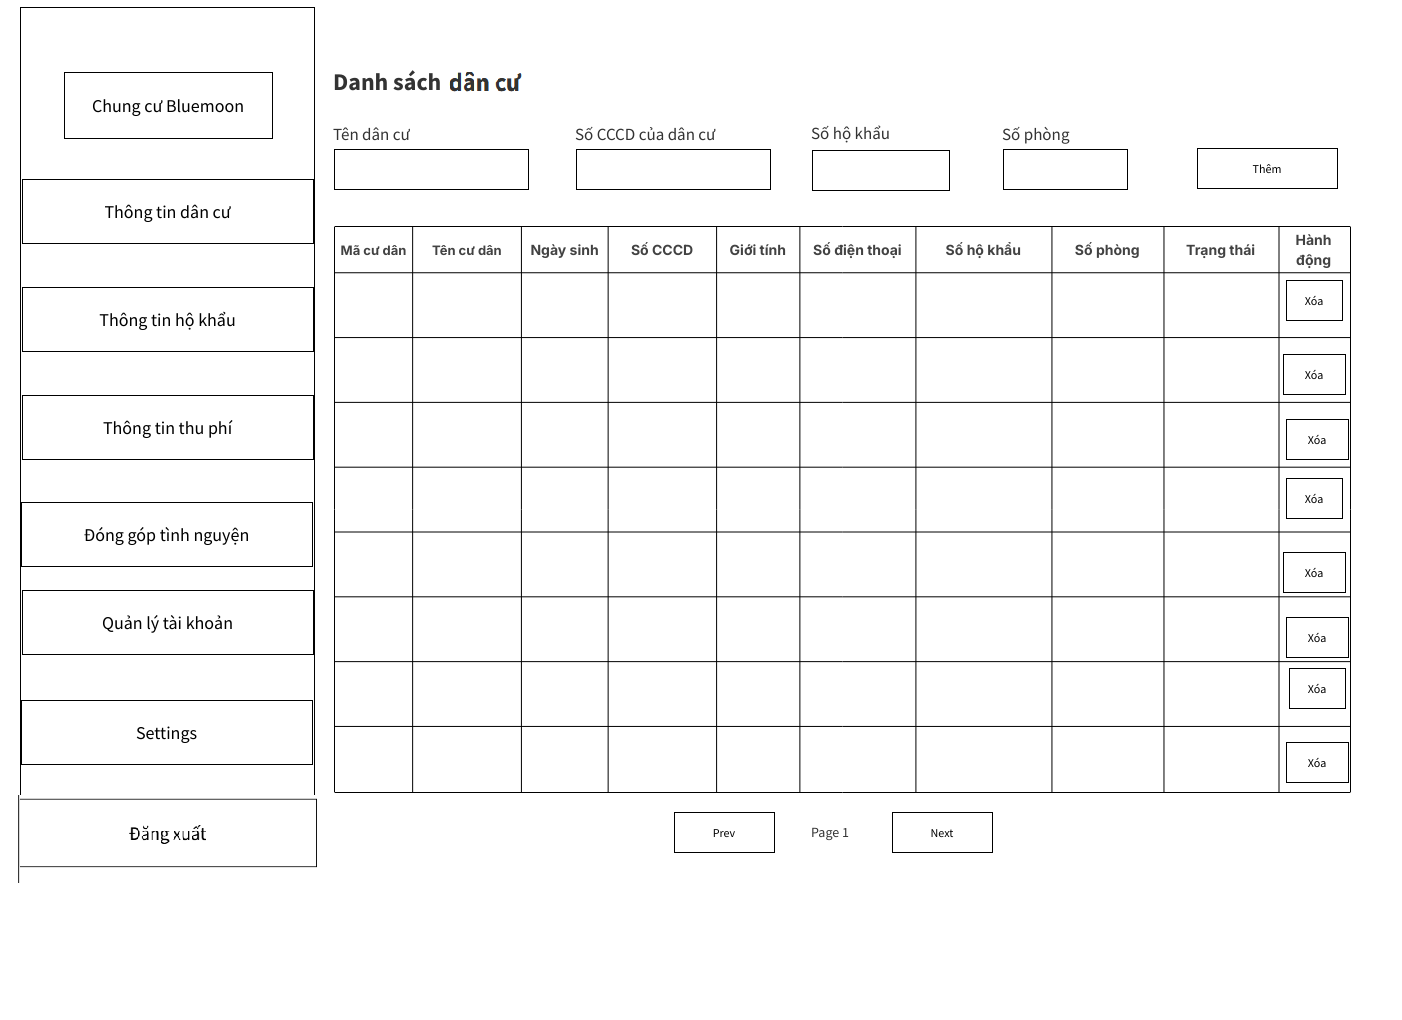
\includegraphics[width=0.9\textwidth]{Ảnh chương 4/Màn hình dân cư.png}
    \end{figure}
    \vspace{2cm}
    \item Mock-up cho màn hình đăng ký nhân khẩu của bài toán (Admin):
    \begin{figure}[H]
        \centering
        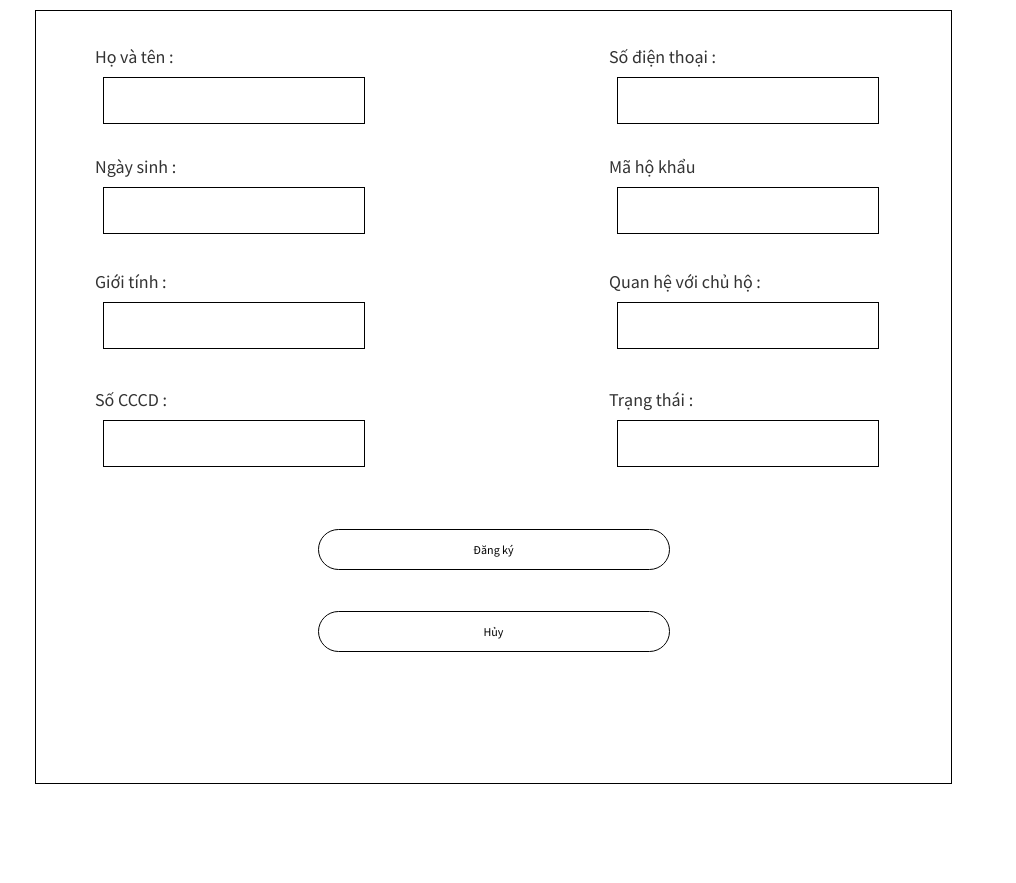
\includegraphics[width=0.8\textwidth]{Ảnh chương 4/Màn hình thêm thông tin dân cư.png}
    \end{figure}
    
    \item Mock-up cho màn hình thông tin dân cư của bài toán (Admin):
    \begin{figure}[H]
        \centering
        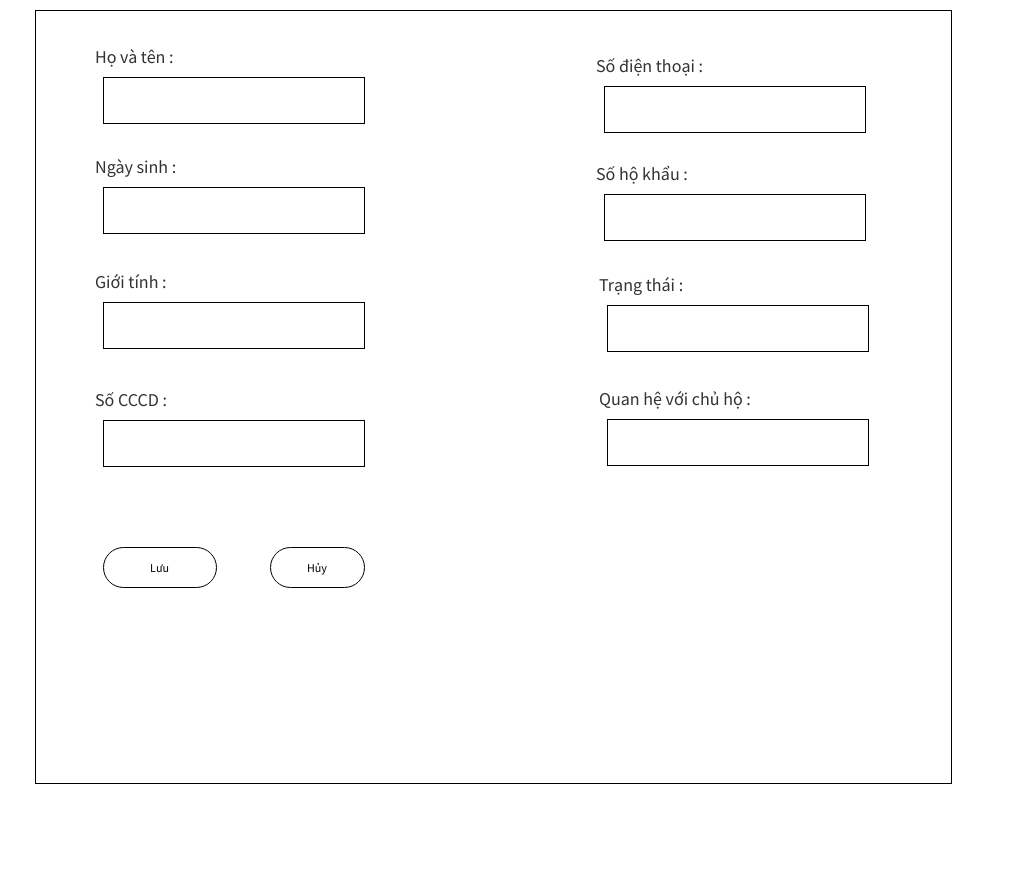
\includegraphics[width=0.8\textwidth]{Ảnh chương 4/Màn hình thông tin cư dân (admin).png}
    \end{figure}
    \item Mock-up cho màn hình thông tin dân cư của bài toán (User):
    \begin{figure}[H]
        \centering
        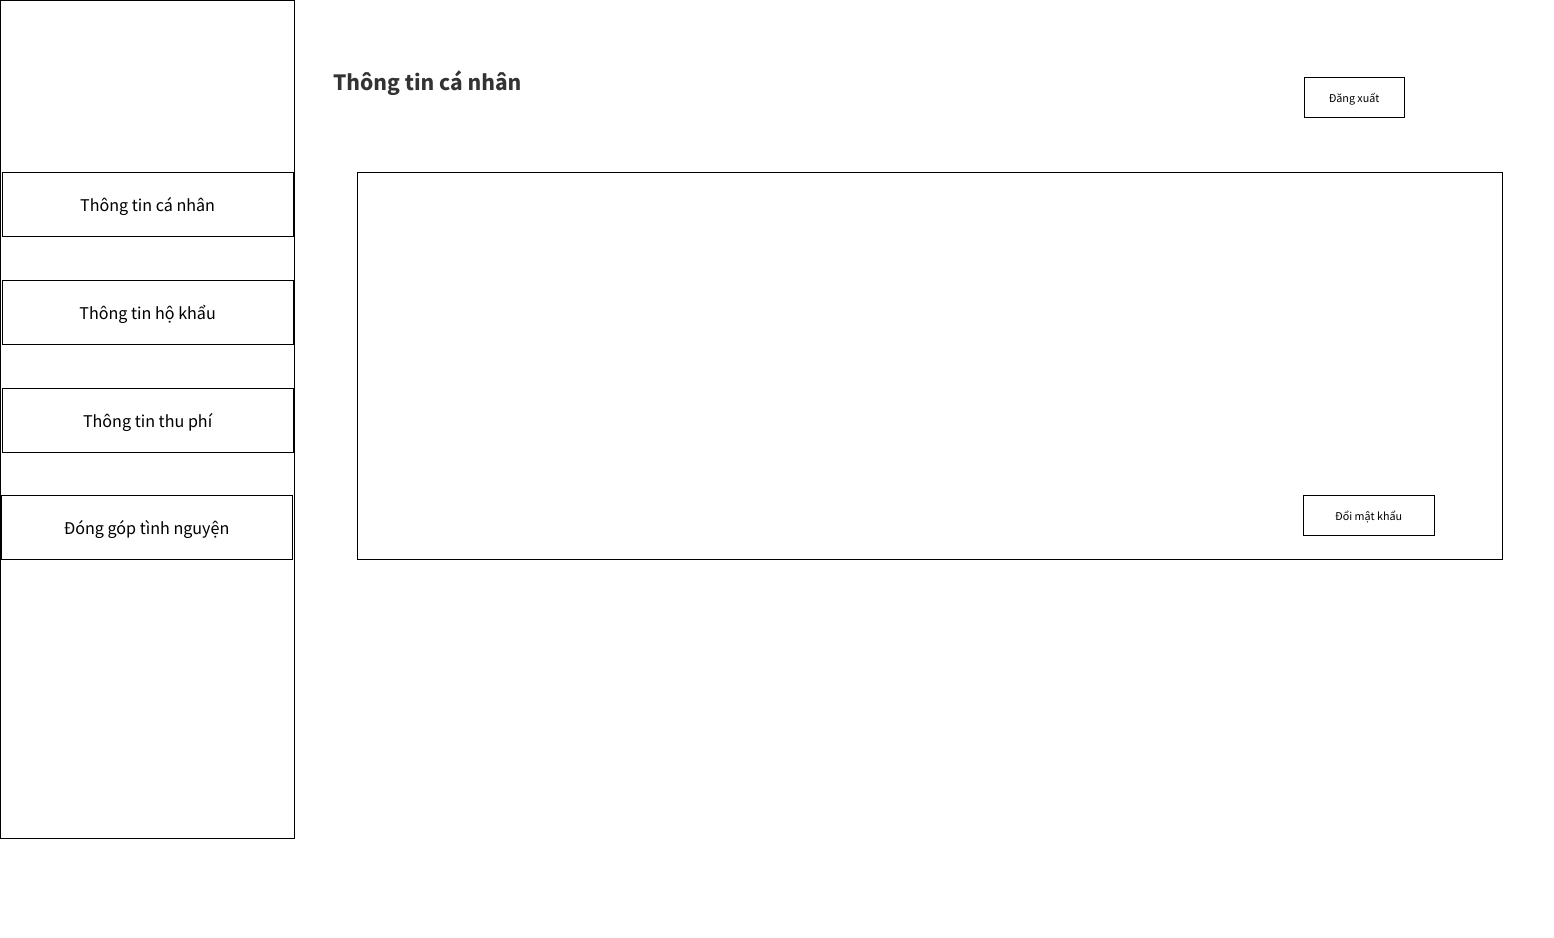
\includegraphics[width=0.9\textwidth]{Ảnh chương 4/Màn hình thông tin cư dân.png}
    \end{figure}
    \item Mock-up cho màn hình thu phí của bài toán (Admin) :
    \begin{figure}[H]
        \centering
        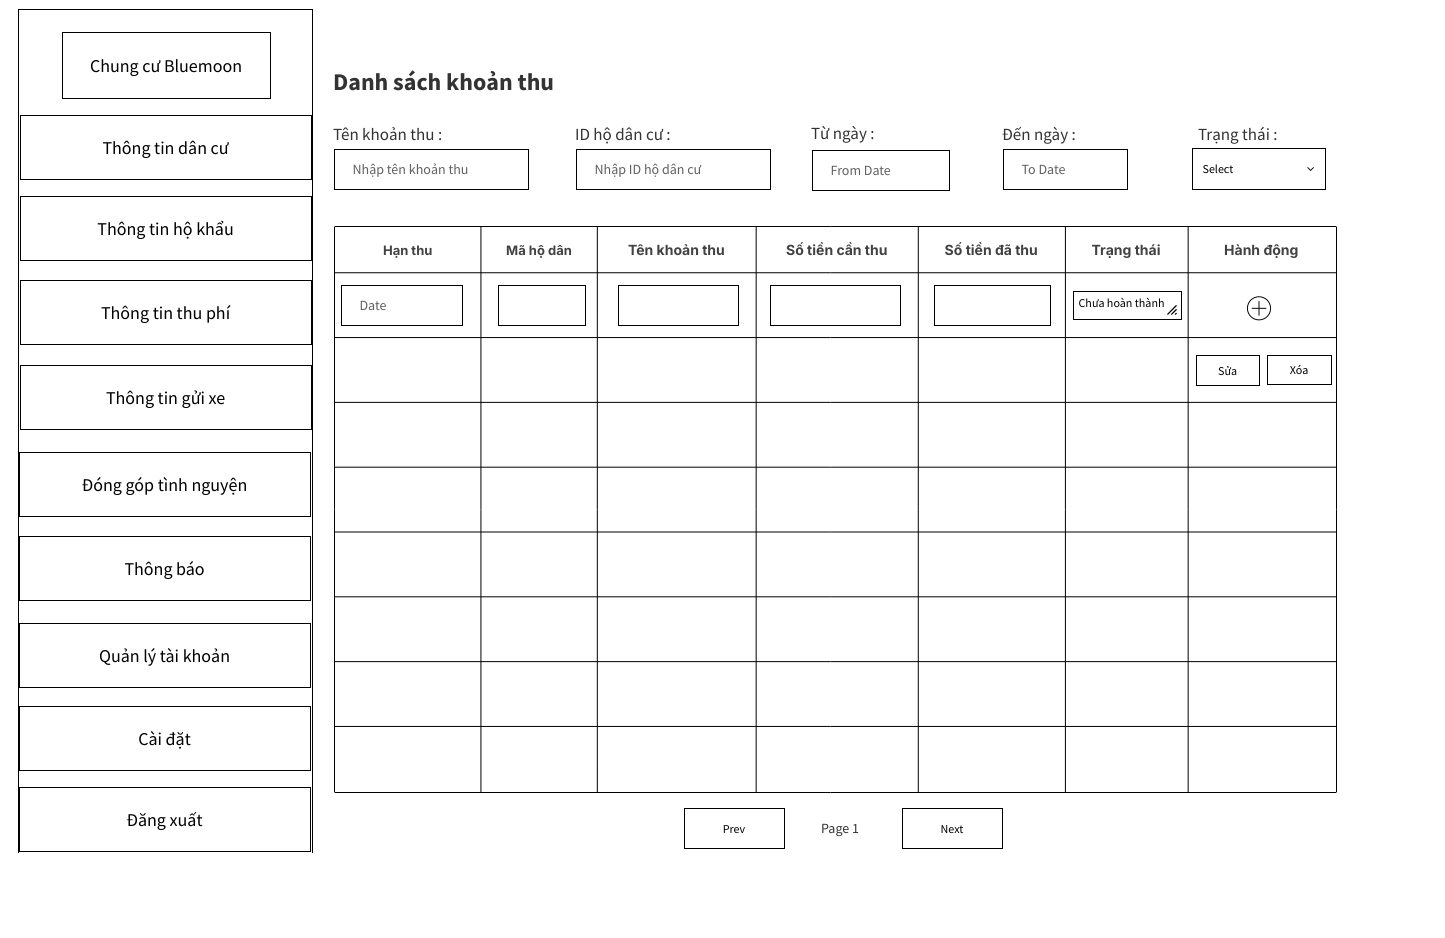
\includegraphics[width=0.9\textwidth]{Ảnh chương 4/Màn hình thu phí.png}
    \end{figure}
    \vspace{3cm}
    \item Mock-up cho màn hình thu phí của bài toán (User) :
    \begin{figure}[H]
        \centering
        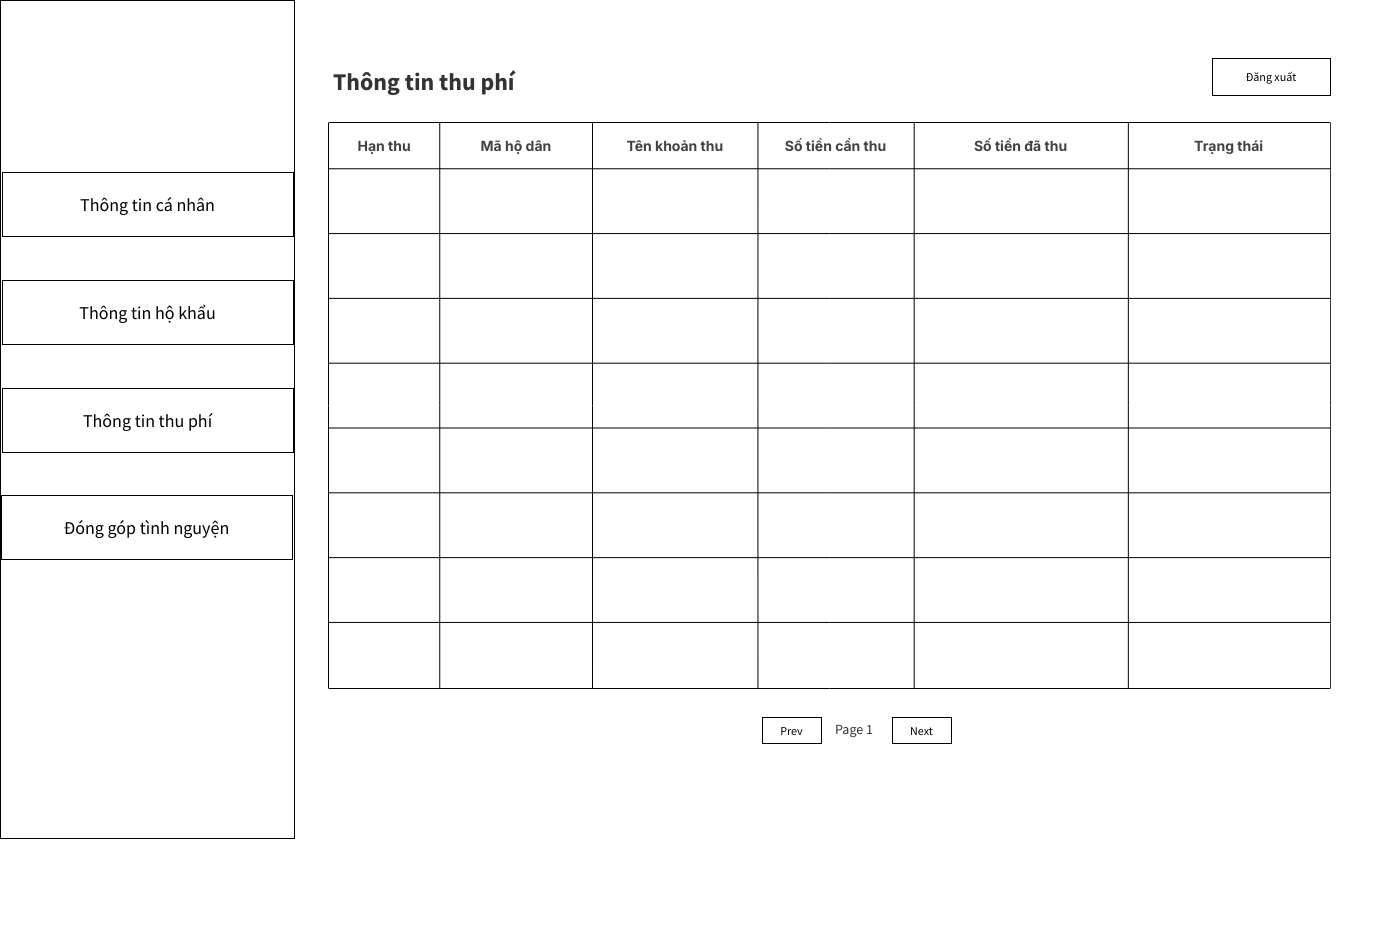
\includegraphics[width=0.9\textwidth]{Ảnh chương 4/Màn hình khoản thu (cư dân).png}
    \end{figure}
    \item Mock-up cho màn hình khoản đóng góp tự nguyện của bài toán (Admin) :
    \begin{figure}[H]
        \centering
        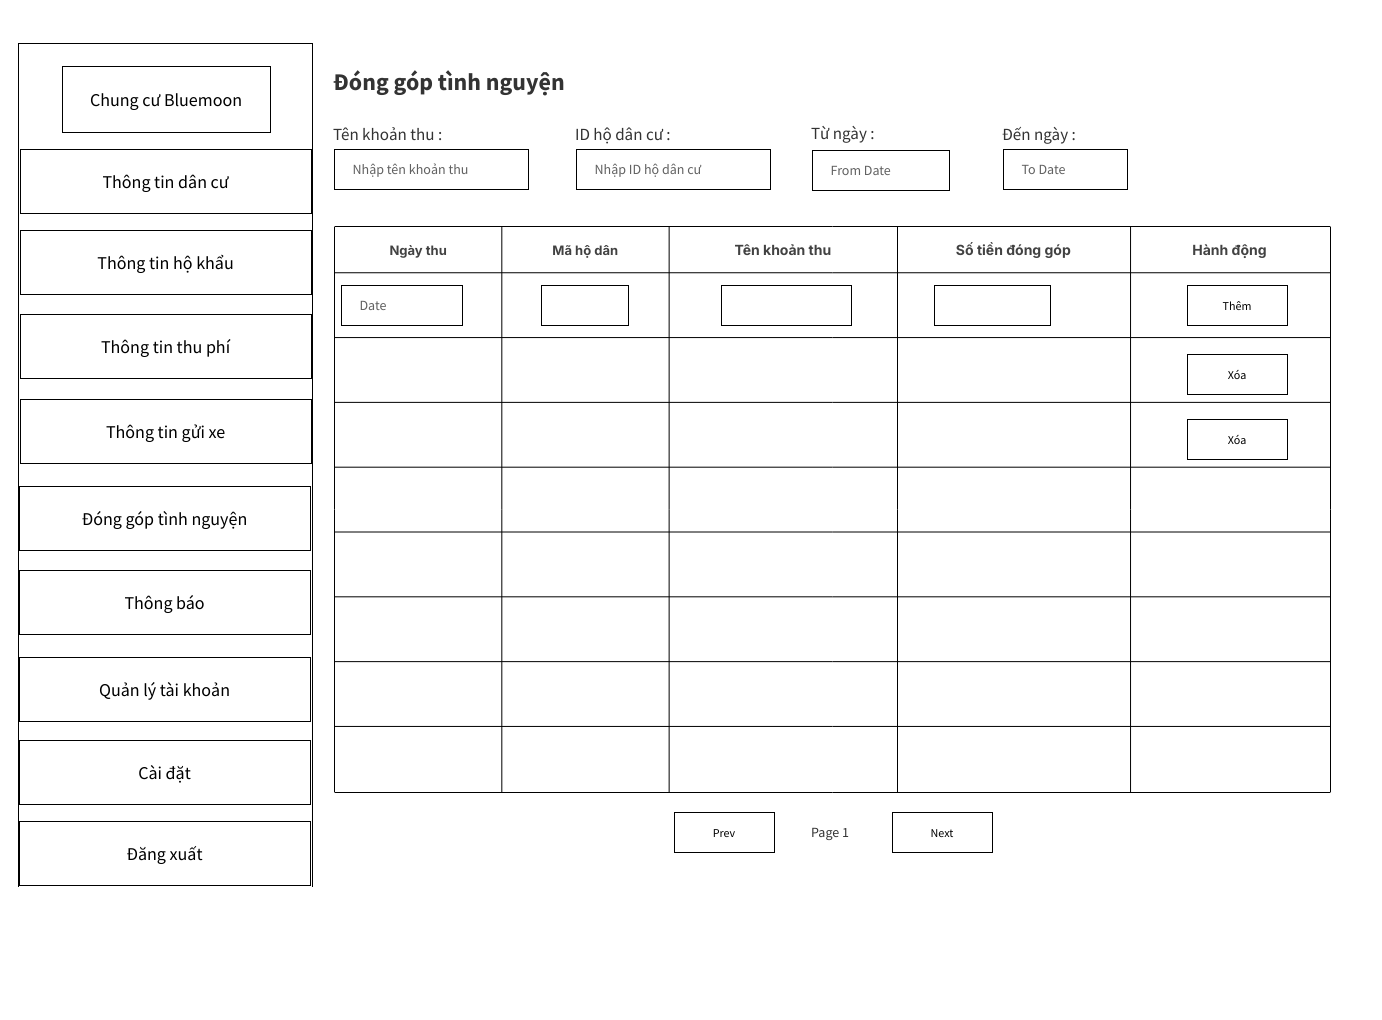
\includegraphics[width=0.9\textwidth]{Ảnh chương 4/Màn hình đóng góp tình nguyện.png}
    \end{figure}
    \vspace{1cm}
    \item Mock-up cho màn hình khoản đóng góp tự nguyện của bài toán (User) :
    \begin{figure}[H]
        \centering
        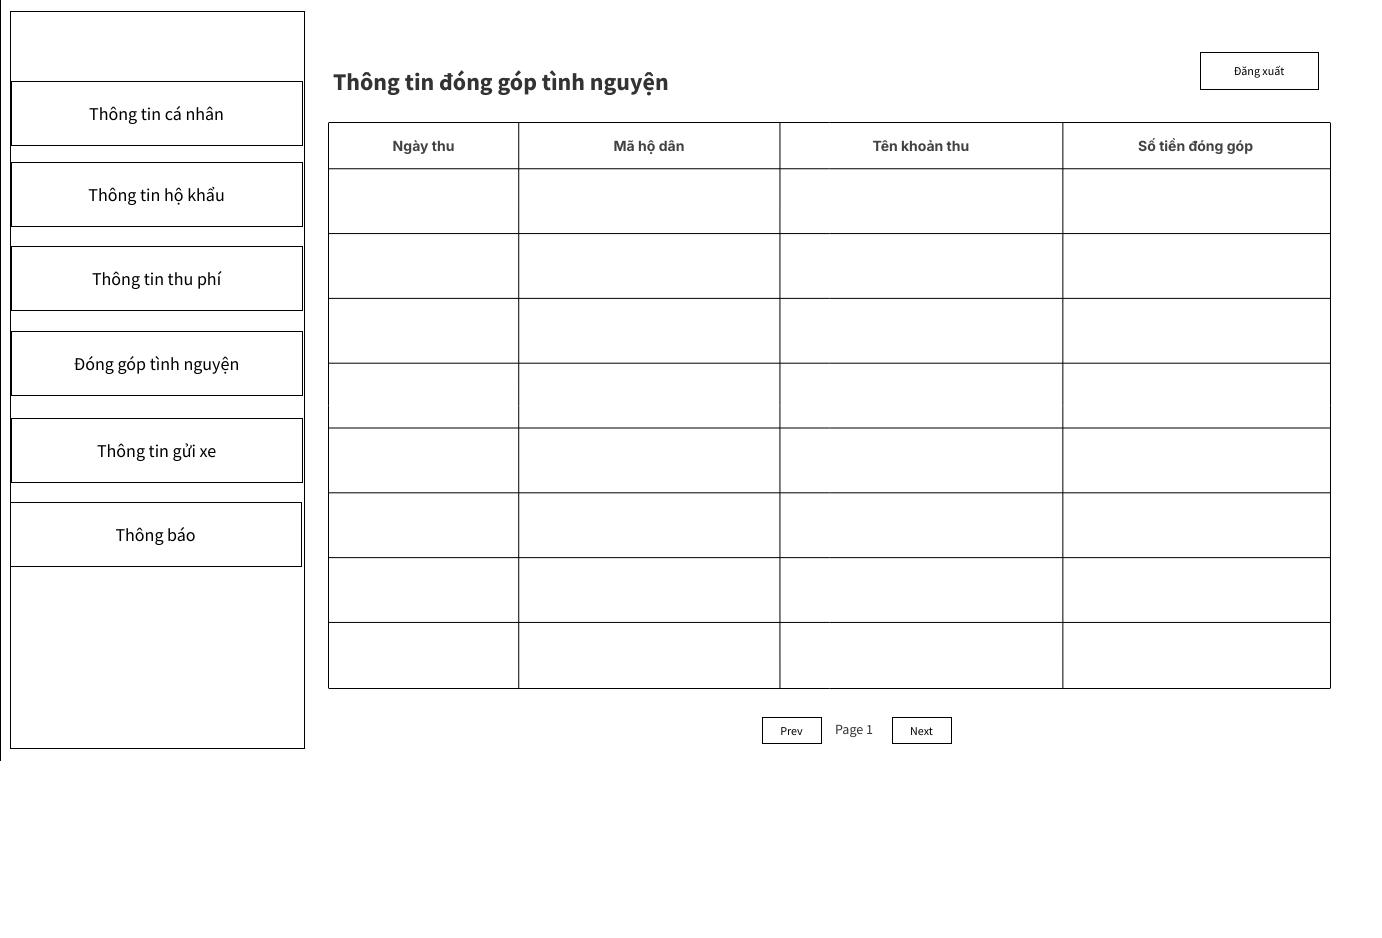
\includegraphics[width=0.9\textwidth]{Ảnh chương 4/Màn hình đóng góp (cư dân).png}
    \end{figure}
    \item Mock-up cho màn hình quản lý tài khoản (Admin) :
    \begin{figure}[H]
        \centering
        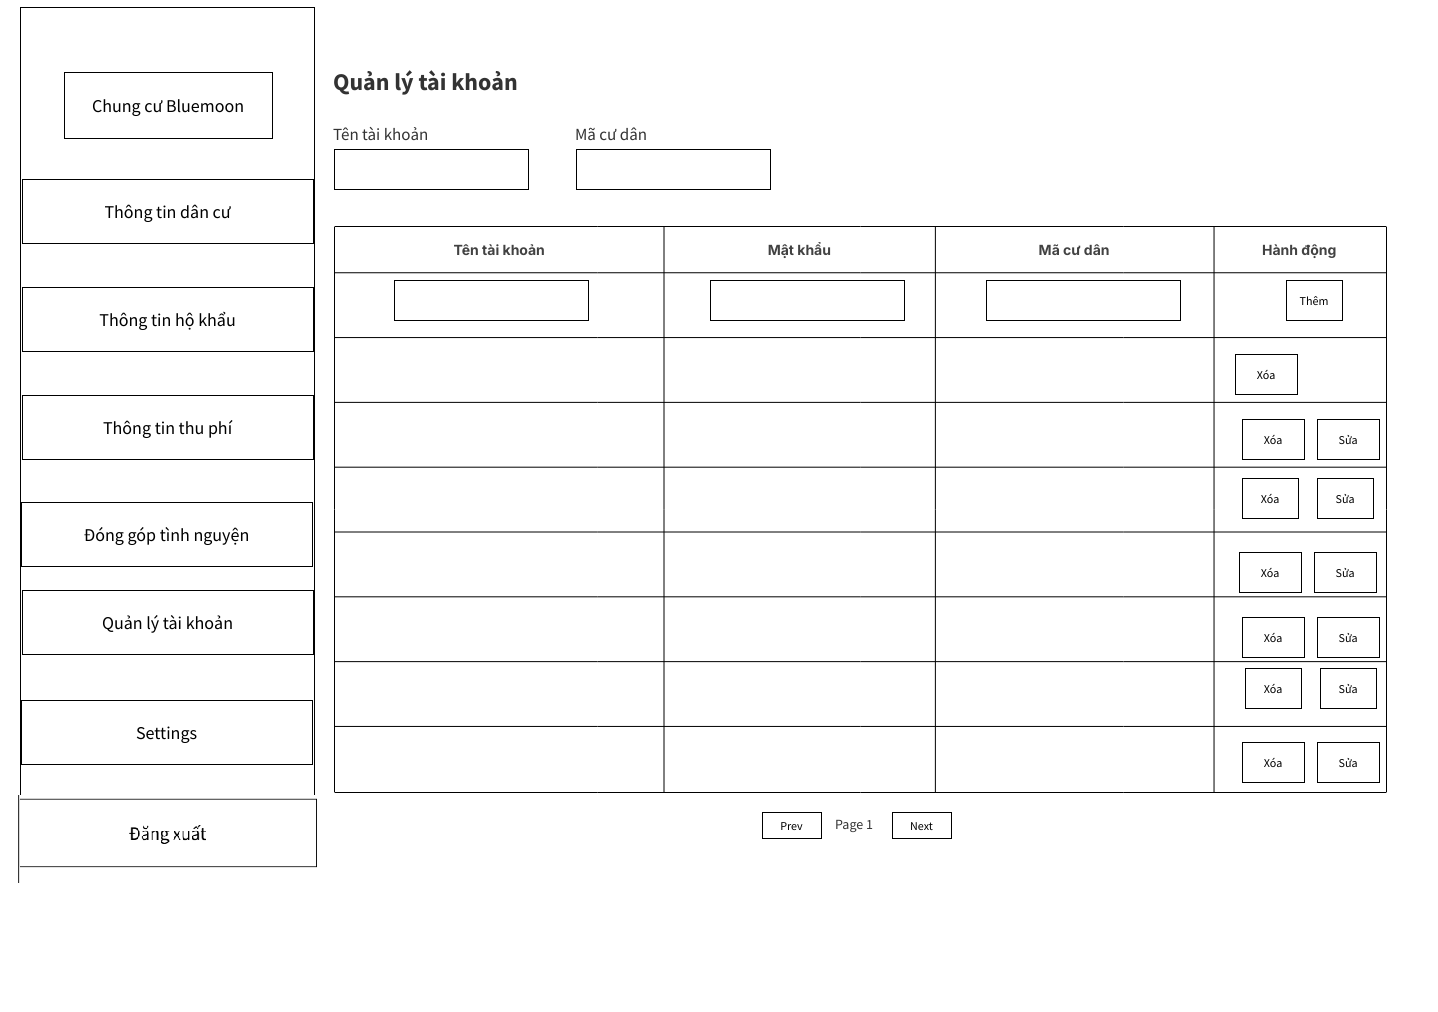
\includegraphics[width=0.9\textwidth]{Ảnh chương 4/Màn hình quản lý tài khoản.png}
    \end{figure}
    \vspace{2cm}
    \item Mock-up cho màn hình cài đặt (Admin):
    \begin{figure}[H]
        \centering
        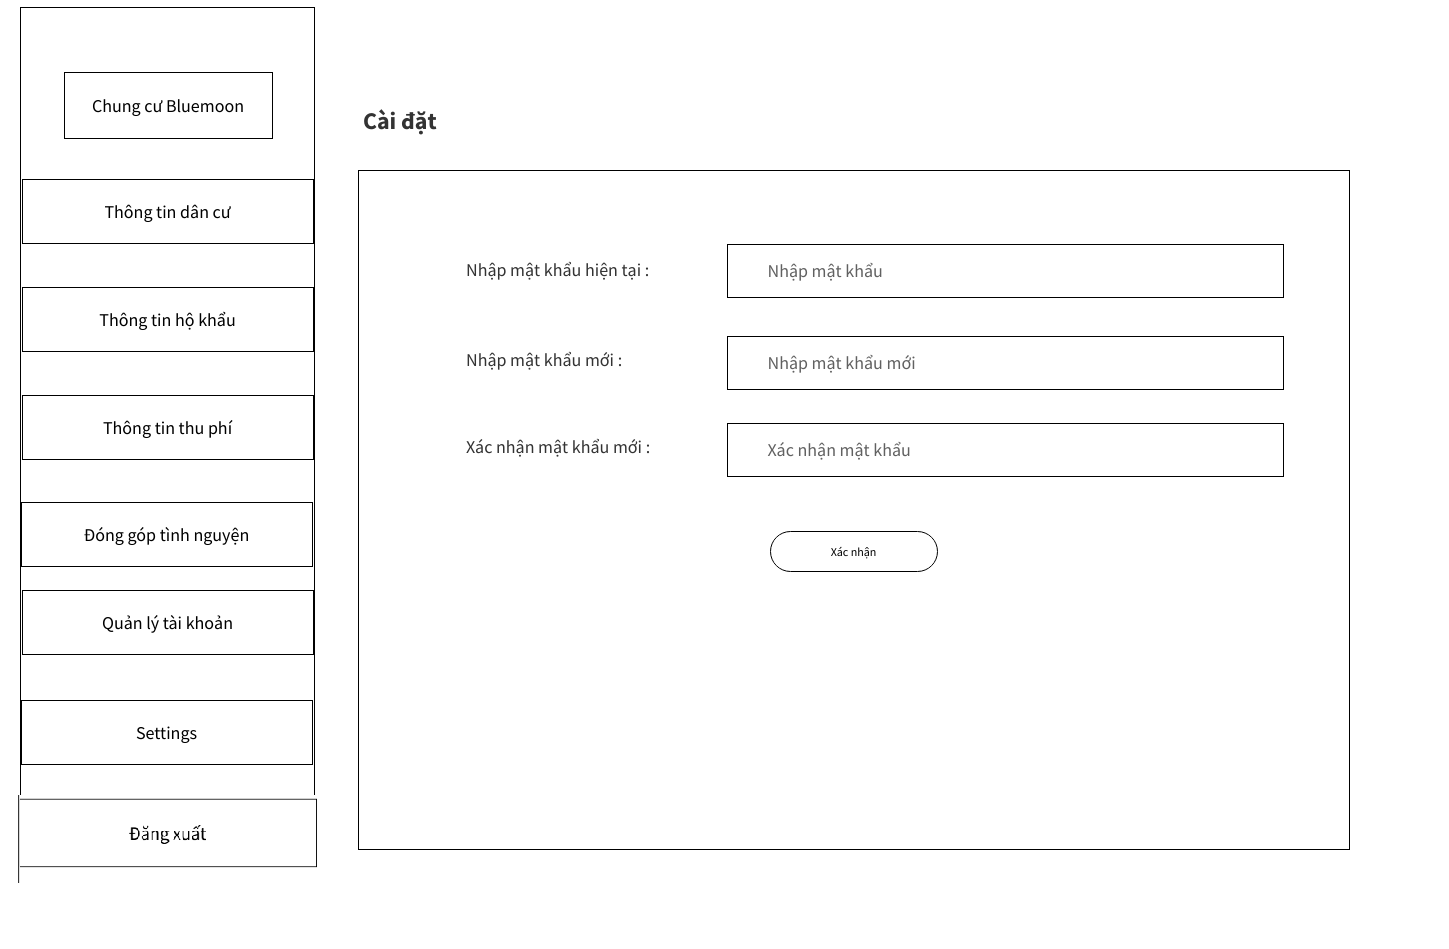
\includegraphics[width=0.9\textwidth]{Ảnh chương 4/Màn hình cài đặt.png}
    \end{figure}
    \item Mock-up cho màn hình cài đặt (User):
    \begin{figure}[H]
        \centering
        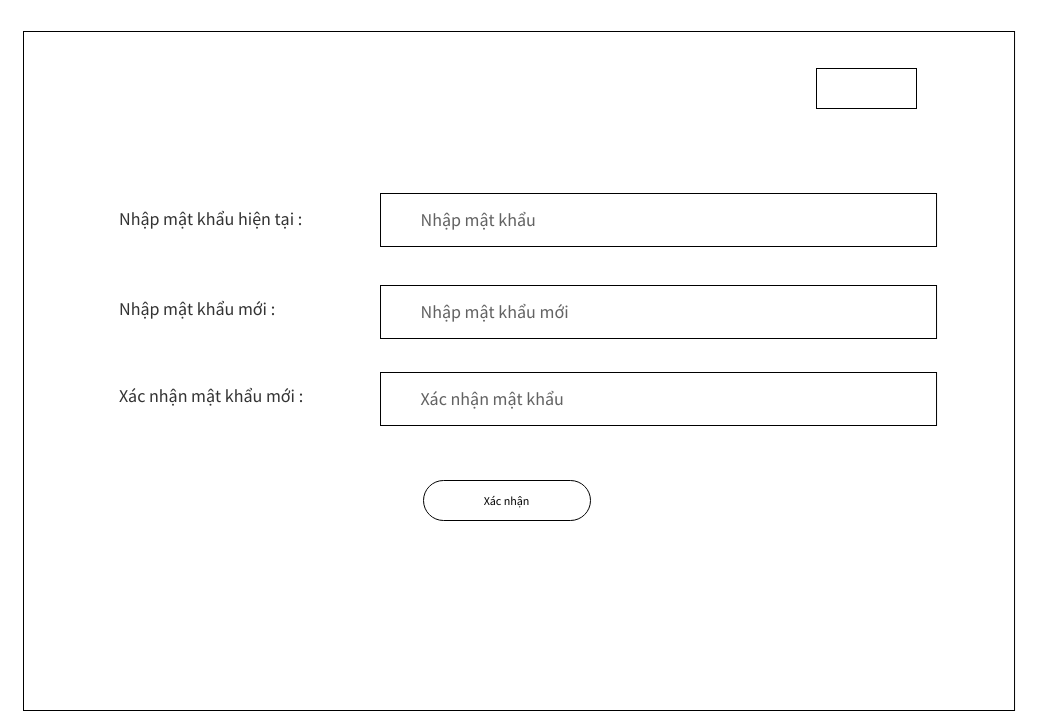
\includegraphics[width=0.9\textwidth]{Ảnh chương 4/Màn hình cài đặt User.png}
    \end{figure}
\end{itemize}
\vspace{3cm}\

\textbf{Đặc tả thiết kế giao diện cho các màn hình}
\begin{itemize}
    \item Giao diện đăng nhập của bài toán :
    \begin{figure}[H]
        \centering
        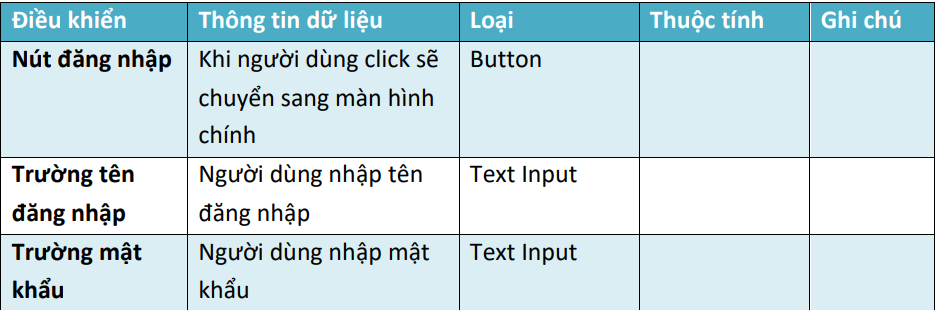
\includegraphics[width=0.8\textwidth]{Ảnh chương 4/Đăng nhập 1.png}
    \end{figure}
    \item Màn hình chính của bài toán :
    \begin{figure}[H]
        \centering
        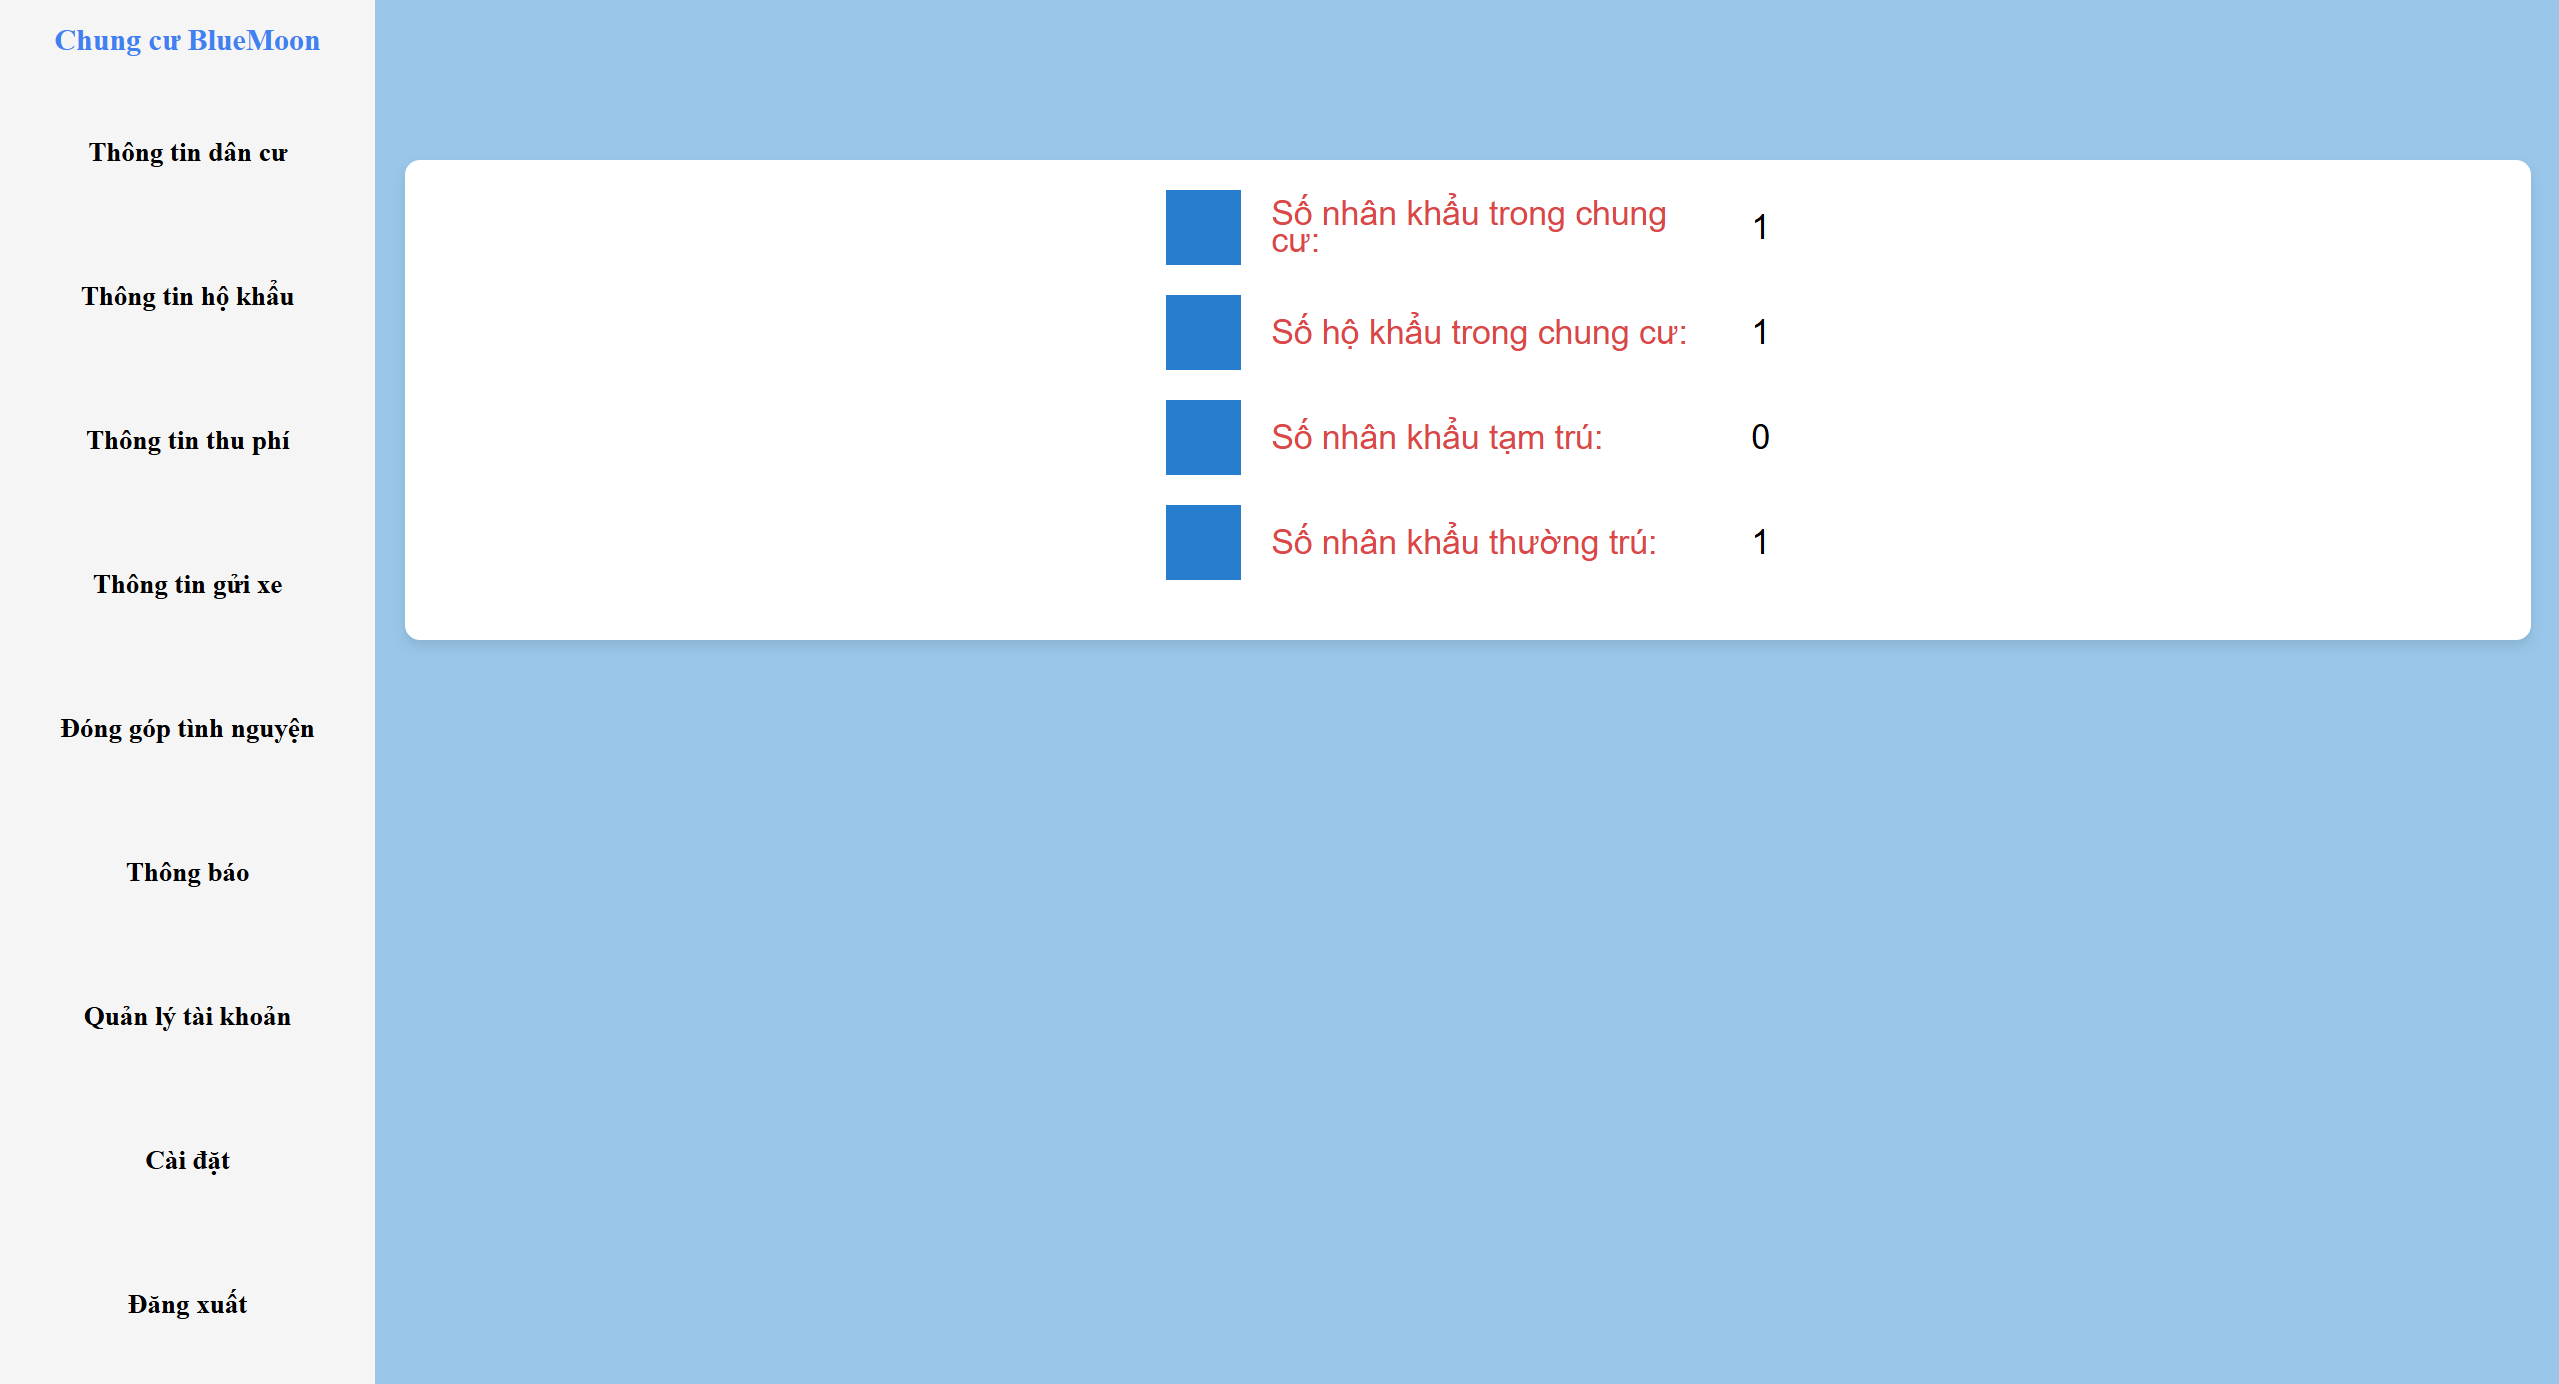
\includegraphics[width=0.8\textwidth]{Ảnh chương 4/Màn hình chính 1.png}
    \end{figure}
    \vspace{1cm}
    \item Màn hình hộ khẩu của bài toán (Admin):
    \begin{figure}[H]
        \centering
        \includegraphics[width=0.8\textwidth]{Ảnh chương 4/Hộ khẩu Admin 1.png}
    \end{figure}
    \begin{figure}[H]
        \centering
        \includegraphics[width=0.8\textwidth]{Ảnh chương 4/Hộ khẩu Admin 2.png}
    \end{figure}
    \item Màn hình hộ khẩu của bài toán (User):
    \begin{figure}[H]
        \centering
        \includegraphics[width=0.8\textwidth]{Ảnh chương 4/Hộ khẩu User 1.png}
    \end{figure}
    \vspace{4cm}
    \item Màn hình xem thông tin chi tiết hộ khẩu của bài toán (Admin):
    \begin{figure}[H]
        \centering
        \includegraphics[width=0.9\textwidth]{Ảnh chương 4/Thông tin hộ khẩu Admin 1.png}
    \end{figure}
    \item Màn hình thêm hộ khẩu của bài toán (Admin):
    \begin{figure}[H]
        \centering
        \includegraphics[width=0.9\textwidth]{Ảnh chương 4/Thêm hộ khẩu 1.png}
    \end{figure}
    \item Màn hình chuyển hộ khẩu của bài toán (Admin):
    \begin{figure}[H]
        \centering
        \includegraphics[width=0.9\textwidth]{Ảnh chương 4/Chuyẻn hộ khẩu 1.png}
    \end{figure}
    \vspace{3cm}
    \item Màn hình nhân khẩu của bài toán (Admin):
    \begin{figure}[H]
        \centering
        \includegraphics[width=0.9\textwidth]{Ảnh chương 4/Dân cư Admin 1.png}
    \end{figure}
        \begin{figure}[H]
        \centering
        \includegraphics[width=0.9\textwidth]{Ảnh chương 4/Dân cư Admin 2.png}
    \end{figure}
    \item Màn hình đăng ký nhân khẩu của bài toán (Admin):
    \begin{figure}[H]
        \centering
        \includegraphics[width=0.9\textwidth]{Ảnh chương 4/Đăng ký nhân khẩu 1.png}
    \end{figure}
    \vspace{5cm}
    \item Màn hình thông tin dân cư của bài toán (Admin):
    \begin{figure}[H]
        \centering
        \includegraphics[width=0.9\textwidth]{Ảnh chương 4/Thông tin dân cư 1.png}
    \end{figure}
    \item Màn hình thông tin dân cư của bài toán (User):
    \begin{figure}[H]
        \centering
        \includegraphics[width=0.9\textwidth]{Ảnh chương 4/Thông tin dân cư User 1.png}
    \end{figure}
    \vspace{1cm}
    \item Màn hình thu phí của bài toán (Admin) :
    \begin{figure}[H]
        \centering
        \includegraphics[width=0.9\textwidth]{Ảnh chương 4/Thu phí Admin 1.png}
    \end{figure}
    \begin{figure}[H]
        \centering
        \includegraphics[width=0.9\textwidth]{Ảnh chương 4/Thông tin thu phí Admin 2.png}
    \end{figure}
    \item Màn hình thu phí của bài toán (User) :
    \begin{figure}[H]
        \centering
        \includegraphics[width=0.9\textwidth]{Ảnh chương 4/Khoản thu User 1.png}
    \end{figure}
    \item Màn hình quản lý tài khoản (Admin) :
    \begin{figure}[H]
        \centering
        \includegraphics[width=0.75\textwidth]{Ảnh chương 4/Quản lý tài khoản Admin 1.png}
    \end{figure}
    \item Màn hình sửa đổi thông tin tài khoản (Admin) :
    \begin{figure}[H]
        \centering
        \includegraphics[width=0.75\textwidth]{Ảnh chương 4/Sửa đổi tài khoản 1.png}
    \end{figure}
    \item Màn hình cài đặt (Admin):
    \begin{figure}[H]
        \centering
        \includegraphics[width=0.9\textwidth]{Ảnh chương 4/Đổi mật khẩu Admin 1.png}
    \end{figure}
    \vspace{3cm}
    \item Màn hình cài đặt (User):
    \begin{figure}[H]
        \centering
        \includegraphics[width=0.9\textwidth]{Ảnh chương 4/Đổi mật khẩu User 1.png}
    \end{figure}
\end{itemize}
\newpage
%---------------------------------------------------------------------
\section*{CHƯƠNG 5. XÂY DỰNG CHƯƠNG TRÌNH MINH HỌA}
\addcontentsline{toc}{section}{CHƯƠNG 5. XÂY DỰNG CHƯƠNG TRÌNH MINH HỌA}
\setcounter{section}{5}
\setcounter{subsection}{0}
\subsection{Thư viện và công cụ sử dụng}
\begin{center}
    \textbf{Danh sách thư viện và công cụ sử dụng} \\
    \begin{tabular}{|c|c|c|}
        \hline
        \textbf{Mục đích} & \textbf{Công cụ} & \textbf{Địa chỉ URL} \\
        \hline
        IDE Lập trình & IntelliJ IDEA & https://lp.jetbrains.com\\
        \hline
        Thư viện & Java Spring Boot & https://spspring.io\\
         & Java Scripts & https://www.javascript.com/\\
         & HTML, CSS & \\
        \hline
    \end{tabular}
\end{center}
\subsection{Kết quả chương trình minh họa}
Chương trình quản lý dân cư và thu phí là một giải pháp số hóa, hỗ trợ các tổ chức và cơ quan quản lý thực hiện hiệu quả các nhiệm vụ như:

\begin{itemize}
    \item Theo dõi thông tin cư dân.
    \item Quản lý tài khoản người dùng.
    \item Xử lý và cập nhật dữ liệu tài chính liên quan đến việc thu phí dịch vụ.
\end{itemize}
 \textbf{Mục tiêu của chương trình}
\begin{enumerate}
    \item \textbf{Tự động hóa quy trình}:
Giảm thiểu khối lượng công việc thủ công thông qua việc ứng dụng công nghệ, tiết kiệm thời gian và công sức.
    \item \textbf{Đảm bảo minh bạch và chính xác}:
Các dữ liệu cư dân, khoản phí và lịch sử giao dịch đều được lưu trữ rõ ràng, dễ dàng truy xuất và kiểm tra.
    \item \textbf{Tăng trải nghiệm người dùng}:
Cư dân có thể dễ dàng tra cứu thông tin tài khoản, thanh toán và cập nhật hồ sơ một cách nhanh chóng, chính xác.
\end{enumerate}
 \textbf{Chức năng nổi bật}
\begin{enumerate}
    \item \textbf{Quản lý tài khoản cư dân}:
Cung cấp giao diện đơn giản để tạo, sửa, xóa thông tin người dùng.
Phân quyền tài khoản (ADMIN, USER) đảm bảo hệ thống an toàn và bảo mật.
    \item \textbf{Thu phí dịch vụ}:
Ghi nhận thông tin các khoản phí dịch vụ theo từng cư dân, bao gồm phí quản lý, điện nước, và các dịch vụ khác.
    \item \textbf{Phân trang và lọc dữ liệu}:
Hỗ trợ quản lý dữ liệu cư dân lớn nhờ tính năng phân trang và tìm kiếm theo các tiêu chí như tên, mã cư dân.
    \item \textbf{Bảo mật thông tin}:
Sử dụng mã hóa mật khẩu với công nghệ tiên tiến (BCrypt), đảm bảo dữ liệu người dùng được bảo vệ tốt nhất.
\end{enumerate}
 \textbf{Kết quả kỳ vọng}\\
Chương trình giúp nâng cao hiệu quả quản lý, tối ưu hóa quy trình thu phí và mang lại sự hài lòng cho cư dân cũng như đội ngũ quản lý. Đây là một bước tiến quan trọng hướng tới quản lý thông minh và bền vững trong thời đại công nghệ số.

\subsection{Giao diện minh hoạ các chức năng của chương trình}

Thiết kế giao diện thực tế cho bài toán:
\begin{itemize}
    \item Màn hình giao diện đăng nhập của bài toán :
    \begin{figure}[H]
        \centering
        \includegraphics[width=1\textwidth]{Ảnh chương 4/Login.png}
    \end{figure}
    \vspace{7cm}
    \item Màn hình chính của bài toán :
    \begin{figure}[H]
        \centering
        \includegraphics[width=1\textwidth]{Ảnh chương 4/Home Admin.png}
    \end{figure}
    \vspace{1cm}
    \item Màn hình hộ khẩu của bài toán (Admin):
    \begin{figure}[H]
        \centering
        \includegraphics[width=1\textwidth]{Ảnh chương 4/Thông tin hộ khẩu Admin.png}
    \end{figure}
    \vspace{4cm}
    \item Màn hình hộ khẩu của bài toán (User):
    \begin{figure}[H]
        \centering
        \includegraphics[width=1\textwidth]{Ảnh chương 4/Thông tin hộ khẩu User.png}
    \end{figure}
    \vspace{1cm}
    \item Màn hình xem thông tin chi tiết hộ khẩu của bài toán (Admin):
    \begin{figure}[H]
        \centering
        \includegraphics[width=1\textwidth]{Ảnh chương 4/Thông tin hộ khẩu Admin.png}
    \end{figure}
    \vspace{5cm}
    \item Màn hình thêm hộ khẩu của bài toán (Admin):
    \begin{figure}[H]
        \centering
        \includegraphics[width=0.8\textwidth]{Ảnh chương 4/Thêm hộ khẩu Admin.png}
    \end{figure}
    \item Màn hình chuyển hộ khẩu của bài toán (Admin):
    \begin{figure}[H]
        \centering
        \includegraphics[width=0.9\textwidth]{Ảnh chương 4/Chuyển hộ khẩu Admin.png}
    \end{figure}
    \item Màn hình nhân khẩu của bài toán (Admin):
    \begin{figure}[H]
        \centering
        \includegraphics[width=0.8\textwidth]{Ảnh chương 4/Admin dân cư.png}
    \end{figure}
    \item Màn hình đăng ký nhân khẩu của bài toán (Admin):
    \begin{figure}[H]
        \centering
        \includegraphics[width=1\textwidth]{Ảnh chương 4/Thêm cư dân admin.png}
    \end{figure}
    \vspace{1cm}
    \item Màn hình thông tin dân cư của bài toán (Admin):
    \begin{figure}[H]
        \centering
        \includegraphics[width=1\textwidth]{Ảnh chương 4/Thông tin cư dân Admin.png}
    \end{figure}
    \vspace{4cm}
    \item Màn hình thông tin dân cư của bài toán (User):
    \begin{figure}[H]
        \centering
        \includegraphics[width=1\textwidth]{Ảnh chương 4/Thông tin cư dân User.png}
    \end{figure}
    \vspace{2cm}
    \item Màn hình thu phí của bài toán (Admin) :
    \begin{figure}[H]
        \centering
        \includegraphics[width=1\textwidth]{Ảnh chương 4/Thông tin thu phí Admin.png}
    \end{figure}
    \vspace{3cm}
    \item Màn hình thu phí của bài toán (User) :
    \begin{figure}[H]
        \centering
        \includegraphics[width=1\textwidth]{Ảnh chương 4/Thông tin thu phí User.png}
    \end{figure}
    \vspace{2cm}
    \item Màn hình khoản đóng góp tự nguyện của bài toán (Admin) :
    \begin{figure}[H]
        \centering
        \includegraphics[width=1\textwidth]{Ảnh chương 4/Tình nguyện Admin.png}
    \end{figure}
    \vspace{2cm}
    \item Màn hình khoản đóng góp tự nguyện của bài toán (User) :
    \begin{figure}[H]
        \centering
        \includegraphics[width=1\textwidth]{Ảnh chương 4/Tình nguyện User.png}
    \end{figure}
    \vspace{2cm}
    \item Màn hình quản lý tài khoản (Admin) :
    \begin{figure}[H]
        \centering
        \includegraphics[width=1\textwidth]{Ảnh chương 4/Quản lý tài khoản Admin.png}
    \end{figure}
    \vspace{2cm}
    \item Màn hình sửa đổi thông tin tài khoản (Admin) :
    \begin{figure}[H]
        \centering
        \includegraphics[width=1\textwidth]{Ảnh chương 4/Sửa đổi tài khoản Admin.png}
    \end{figure}
    \vspace{1cm}
    \item Màn hình cài đặt (Admin):
    \begin{figure}[H]
        \centering
        \includegraphics[width=1\textwidth]{Ảnh chương 4/Màn hình đổi mật khẩu Admin.png}
    \end{figure}
    \vspace{3cm}
    \item Màn hình cài đặt (User):
    \begin{figure}[H]
        \centering
        \includegraphics[width=1\textwidth]{Ảnh chương 4/Màn hình đổi mật khẩu User.png}
    \end{figure}
\end{itemize}
\newpage

%---------------------------------------------------------------------
\section*{CHƯƠNG 6. KIỂM THỬ CHƯƠNG TRÌNH}
\addcontentsline{toc}{section}{CHƯƠNG 6. KIỂM THỬ CHƯƠNG TRÌNH}
\setcounter{section}{6}
\setcounter{subsection}{0}
\subsection{Kiểm thử các chức năng đã thực hiện}
\subsubsection{Kiểm thử cho chức năng quản lý nhân khẩu}
\begin{itemize}
    \item Chức năng thêm mới nhân khẩu
    \begin{figure}[H]
        \centering
        \includegraphics[width=1\textwidth]{Kiểm thử nhân khẩu/Screenshot 2024-12-13 235715.png}
    \end{figure}
    \item Chức năng xóa nhân khẩu:
    \begin{figure}[H]
        \centering
        \includegraphics[width=1\textwidth]{Kiểm thử nhân khẩu/Screenshot 2024-12-13 235722.png}
    \end{figure}
    \item Chức năng sửa nhân khẩu:
    \begin{figure}[H]
        \centering
        \includegraphics[width=1\textwidth]{Kiểm thử nhân khẩu/Screenshot 2024-12-13 235731.png}
    \end{figure}
    \vspace{2cm}
    \item Chức năng tìm kiếm nhân khẩu:
    \begin{figure}[H]
        \centering
        \includegraphics[width=1\textwidth]{Kiểm thử nhân khẩu/Screenshot 2024-12-13 235737.png}
    \end{figure}
    \item Chức năng xem thông tin nhân khẩu:
    \begin{figure}[H]
        \centering
        \includegraphics[width=1\textwidth]{Kiểm thử nhân khẩu/Screenshot 2024-12-13 235745.png}
    \end{figure}
\end{itemize}
\subsubsection{Kiểm thử cho chức năng quản lý hộ khẩu}
\begin{itemize}
    \item Chức năng thêm mới hộ khẩu
    \begin{figure}[H]
        \centering
        \includegraphics[width=1\textwidth]{Kiểm thử hộ khẩu/Screenshot 2024-12-14 001936.png}
    \end{figure}
    \item Chức năng xóa hộ khẩu:
    \begin{figure}[H]
        \centering
        \includegraphics[width=1\textwidth]{Kiểm thử hộ khẩu/Screenshot 2024-12-14 001941.png}
    \end{figure}
    \vspace{1cm}
    \item Chức năng xem thông tin hộ khẩu:
    \begin{figure}[H]
        \centering
        \includegraphics[width=1\textwidth]{Kiểm thử hộ khẩu/Screenshot 2024-12-14 001946.png}
    \end{figure}
    \item Chức năng tìm kiếm hộ khẩu:
    \begin{figure}[H]
        \centering
        \includegraphics[width=1\textwidth]{Kiểm thử hộ khẩu/Screenshot 2024-12-14 001954.png}
    \end{figure}
    \item Chức năng chuyển hộ khẩu:
    \begin{figure}[H]
        \centering
        \includegraphics[width=1\textwidth]{Kiểm thử hộ khẩu/Screenshot 2024-12-14 002001.png}
    \end{figure}
\end{itemize}
\subsubsection{Kiểm thử cho chức năng quản lý khoản thu tự nguyện}
\begin{itemize}
    \item Chức năng tìm kiếm khoản thu:
    \begin{figure}[H]
        \centering
        \includegraphics[width=1\textwidth]{Kiểm thử phí tình nguyện/Screenshot 2024-12-14 002438.png}
    \end{figure}
    \vspace{2cm}
    \item Chức năng xóa khoản thu:
    \begin{figure}[H]
        \centering
        \includegraphics[width=1\textwidth]{Kiểm thử phí tình nguyện/Screenshot 2024-12-14 002443.png}
    \end{figure}
    \item Chức năng thêm khoản thu:
    \begin{figure}[H]
        \centering
        \includegraphics[width=1\textwidth]{Kiểm thử phí tình nguyện/Screenshot 2024-12-14 002453.png}
    \end{figure}
\end{itemize}
\subsubsection{Kiểm thử cho chức năng quản lý khoản thu bắt buộc}
\begin{itemize}
    \item Chức năng thêm mới khoản thu :
    \begin{figure}[H]
        \centering
        \includegraphics[width=1\textwidth]{Kiểm thử phí bắt buộc/Screenshot 2024-12-14 002802.png}
    \end{figure}
    \item Chức năng cập nhật khoản thu:
    \begin{figure}[H]
        \centering
        \includegraphics[width=1\textwidth]{Kiểm thử phí bắt buộc/Screenshot 2024-12-14 002808.png}
    \end{figure}
    \vspace{1cm}
    \item Chức năng xóa khoản thu:
    \begin{figure}[H]
        \centering
        \includegraphics[width=1\textwidth]{Kiểm thử phí bắt buộc/Screenshot 2024-12-14 002812.png}
    \end{figure}
    \item Chức năng tìm kiếm khoản thu:
    \begin{figure}[H]
        \centering
        \includegraphics[width=1\textwidth]{Kiểm thử phí bắt buộc/Screenshot 2024-12-14 002822.png}
    \end{figure}
\end{itemize}
\subsubsection{Kiểm thử yêu cầu phi chức năng}
\begin{itemize}
    \item Đảm bảo chỉ người dùng có quyền hợp lệ mới truy cập được tài nguyên.
    \item Kiểm tra logic phân quyền theo vai trò (Admin/User) thành công.
    \item Thời gian phản hồi phải nhỏ hơn 2 giây cho các trang chính. 
    \item Đảm bảo website hiển thị chính xác trên các trình duyệt phổ biến như Chrome, Microsoft Edge, ..
\end{itemize}
 
\newpage

%---------------------------------------------------------------------
\section*{CHƯƠNG 7. HƯỚNG DẪN CÀI ĐẶT VÀ SỬ DỤNG}
\addcontentsline{toc}{section}{CHƯƠNG 7. HƯỚNG DẪN CÀI ĐẶT VÀ SỬ DỤNG}
\setcounter{section}{7}
\setcounter{subsection}{0}
\subsection{Hướng dẫn cài đặt}
\begin{itemize}
    \item Để sử dụng phần mềm, cần chuẩn bị môi trường chạy Java Spring Boot.
    \item Cài đặt một số công cụ và thư viện cần thiết như:
    \begin{itemize}
        \item \textbf{JDK} (Java Development Kit) phiên bản 11 trở lên.
        \item \textbf{Maven} để quản lý dự án và thư viện.
        \item \textbf{MySQL Server} để quản lý cơ sở dữ liệu.
        \item \textbf{Thư viện MySQL Connector} cho kết nối cơ sở dữ liệu.
        \item \textbf{Thư viện Frontend} như Bootstrap hoặc các framework JS nếu cần.
    \end{itemize}
    \item Cài đặt IDE hỗ trợ phát triển Java (IntelliJ IDEA, Eclipse, hoặc Visual Studio Code).
\end{itemize}
\subsection{Đối tượng, phạm vi sử dụng}
\begin{itemize} 
    \item \textbf{Đối tượng sử dụng}: Nhân viên quản lý, kế toán hoặc quản trị viên cần theo dõi thông tin cư dân và thực hiện thu phí dịch vụ hoặc cư dân trong chung cư để nắm được thông báo của khu dân cư.
    \item \textbf{Phạm vi sử dụng}: Hệ thống này được thiết kế để quản lý các khoản thu phí và thông tin cư dân tại các khu vực hoặc khu dân cư lớn. 
\end{itemize}
\subsection{Xác định các yêu cầu cài đặt}
\subsubsection{\textbf{Yêu cầu phần mềm}:}
\begin{itemize}
    \item Java JDK 11 hoặc cao hơn.
    \item MySQL Server phiên bản 8.0 trở lên.
    \item Maven để quản lý các thư viện.
    \item Spring Boot Framework (được cấu hình trong dự án).
\end{itemize}
\subsubsection{\textbf{Yêu cầu phần cứng}:}
\begin{itemize}

    \item Dung lượng ổ cứng còn trống: ít nhất 500MB để cài đặt phần mềm và lưu trữ dữ liệu.
\end{itemize}
\subsection{Hướng dẫn chi tiết các bước cài đặt}
\begin{enumerate}
    \item \textbf{Cài đặt Java JDK và thiết lập biến môi trường:}
    \begin{itemize}
        \item Tải JDK từ trang chủ: \href{https://www.oracle.com/java/technologies/javase-jdk11-downloads.html}{https://www.oracle.com/java/technologies/javase-jdk11-downloads.html}.
        \item Sau khi cài đặt, cấu hình biến môi trường \verb|JAVA_HOME| và thêm vào \verb|PATH|.
    \end{itemize}
    \item \textbf{Cài đặt MySQL Server:}
    \begin{itemize}
        \item Tải MySQL Server từ \href{https://dev.mysql.com/downloads/mysql/}{https://dev.mysql.com/downloads/mysql/}.
        \item Sau khi cài đặt, sử dụng MySQL Workbench để tạo cơ sở dữ liệu với file \verb|.sql| có sẵn trong thư mục dự án.
    \end{itemize}
    \item \textbf{Cài đặt Maven:}
    \begin{itemize}
        \item Tải và cài đặt Maven từ \href{https://maven.apache.org/download.cgi}{https://maven.apache.org/download.cgi}.
        \item Cấu hình biến môi trường \verb|MAVEN_HOME| và thêm vào \verb|PATH|.
    \end{itemize}
    \item \textbf{Cấu hình cơ sở dữ liệu trong ứng dụng:}
    \begin{itemize}
        \item Mở file \verb|application.properties| hoặc \verb|application.yml| trong dự án.
        \item Chỉnh sửa các thông tin kết nối:\\
    \verb|spring.datasource.url=jdbc:mysql://localhost:3306/ten_database|
    \verb|spring.datasource.username=ten_user|\\
    \verb|spring.datasource.password=mat_khau|
    \end{itemize}
    \item \textbf{Chạy ứng dụng:}
    \begin{itemize}
        \item Sử dụng lệnh sau để khởi chạy ứng dụng:\\\verb|mvn spring-boot:run |
        \item Ứng dụng sẽ khởi chạy trên cổng mặc định (thường là \verb|http://localhost:8080|).
    \end{itemize}
    \item \textbf{Kiểm tra giao diện web:}
    \begin{itemize}
        \item Mở trình duyệt và truy cập vào URL: \verb|http://localhost:8080|.
        \item Đăng nhập bằng tài khoản quản trị viên mặc định (nếu có) hoặc tài khoản cư dân được cấp.
    \end{itemize}.
\end{enumerate}
\subsection{Hướng dẫn sử dụng phần mềm}
Phần mềm dùng cho kế toán để quản lý thông tin thu phí trong khu vực và dùng cho cư dân xem thông tin liên quan.

Phần mềm có 4 chức năng chính là quản lý nhân khẩu, quản lý hộ khẩu, quản lý khoản phí và quản lý tài khoản. Mỗi chức năng quản lý nhân khẩu, hộ khẩu, tài khoản đều có những chức năng con thêm, sửa, xóa, tìm kiếm thông tin trừ chức năng quản lý khoản phí không có chức năng xóa.

Để sử dụng chức năng nào nhấn trực tiếp vào chức năng đó và sử dụng.
\newpage

%---------------------------------------------------------------------
\section*{KẾT LUẬN VÀ HƯỚNG PHÁT TRIỂN}
\addcontentsline{toc}{section}{KẾT LUẬN VÀ HƯỚNG PHÁT TRIỂN}
Kết thúc quá trình phát triển phần mềm, đa số đã hoàn thành được những yêu cầu đã đặt ra trước đó của nhóm như là giúp xây dựng một phần mềm quản lý thu phí đơn giản, dễ sử dụng, công khai và minh bạch các khoản phí. Những chức năng quản lý nhân khẩu, hộ khẩu, khoản thu, nộp tiền đều hỗ trợ thêm, sửa, xóa, tìm kiếm thông tin, các chức năng đều dễ sử dụng.

Tuy nhiên, do thời gian có hạn nên trong quá trình phát triển cũng còn 1 số phần mà chưa được hợp lý mà chưa thể sửa chữa ngay. Trong phần quản lý các khoản thu, các khoản thu là tự nguyện nhưng số tiền nộp vẫn bị thiết lập mặc định, chưa có thống kê chi tiết về số hộ nộp các khoản phí, số hộ chưa nộp để dễ dàng trong việc quản lý. Ngoài ra, còn một số lỗi nho nhỏ khác mà nhóm có thể chưa phát hiện ra.
Phần mềm nếu hoạt động trên các cơ sở dữ liệu lớn thì sẽ bị chậm.

Trong tương lai, nhóm chúng em sẽ cố gắng hoàn thiện phát triển phần mềm để mang lại một phần mềm có trải nghiệm tốt hơn, khắc phục được những nhược điểm bên trên. Nếu có điều kiện cho phép về thời gian, nhân lực nhóm có thể phát triển phần mềm thêm nhiều chức năng khác để giúp đơn giản hóa các công việc được thực hiện thủ công rất mệt mỏi và dễ bị nhầm lẫn.
\newpage

%---------------------------------------------------------------------
\section*{TÀI LIỆU THAM KHẢO}
\addcontentsline{toc}{section}{TÀI LIỆU THAM KHẢO}
\newpage

%---------------------------------------------------------------------
\section*{PHỤ LỤC}
\addcontentsline{toc}{section}{PHỤ LỤC}

\end{document}
